
%!TEX option = --shell-escape

\documentclass[9pt, xcolor={svgnames, x11names},professionalfonts]{beamer}


\usepackage{xcolor}
\usepackage{cancel}
\usepackage{bm}
\usepackage{graphicx}
\usepackage[x11names, svgnames]{xcolor} % for colors in handouts, auto loaded in Beamer?
\usepackage{tikz}
\usetikzlibrary{arrows.meta, math, calc, shadows}
\usetikzlibrary{decorations.markings, decorations.fractals, decorations.text} % for chain, etc.
\usetikzlibrary{intersections}
\usepackage{pgfmath}
\usepackage{ifthen}
\usepgfmodule{oo}
\usepgflibrary{shadings}
% \usetikzlibrary{decorations.shapes}
\usepackage[many]{tcolorbox}
\usepackage[absolute,overlay,showboxes]{textpos}
% \usepackage{textpos}
% \textblockorigin{0.0cm}{0.0cm}  %start all at upper left corner
\TPshowboxesfalse

\newcommand\lb{\linebreak}
\newcommand\Ra{\Rightarrow}
\newcommand\cd{\!\cdot\!}
\newcommand\x{\!\times\!}
\newcommand\pars{\par\smallskip}
\newcommand\parm{\par\medskip}
\newcommand\parb{\par\bigskip}
\renewcommand{\deg}{^\circ}

% counter for resuming enumerated list numbers
\newcounter{resumeenumi}
\newcommand{\suspend}{\setcounter{resumeenumi}{\theenumi}}
\newcommand{\resume}{\setcounter{enumi}{\theresumeenumi}}



% https://tex.stackexchange.com/questions/33703/extract-x-y-coordinate-of-an-arbitrary-point-in-tikz
\makeatletter
\providecommand{\gettikzxy}[3]{%
	\tikz@scan@one@point\pgfutil@firstofone#1\relax
	\edef#2{\the\pgf@x}%
	\edef#3{\the\pgf@y}%
}
\makeatother

\makeatletter
\newcommand{\verbatimfont}[1]{\def\verbatim@font{#1}}%
\makeatother

%%%%%%%%%%%%%%%%%%%%%%%%%%%%%%%%%%%%%%%%%%%%%%%%%%%%%%%%%%%%%%%%%%%%%%%%%%%%%%%%


\newcommand{\tb}[4][0.8]{
	\begin{textblock*}{#1}(#2, #3)
		% \raggedright
		#4
	\end{textblock*}
}

\newtcolorbox{statsbox}[2][] { 
  colback=white,
  colbacktitle=structure,
  colframe=structure,
  coltitle=white,  
  top=0.25cm,
	bottom=0.125cm,
	left=0mm,
	right=0mm,
  % fonttitle=\itshape\rmfamily,
  halign=flush left, 
  enhanced,
  drop fuzzy shadow,
  attach boxed title to top left={xshift=3.5mm, yshift=-2mm},
  title={#2}, #1}
\newtcolorbox{redbox}{colback=white, colframe=structure, enhanced, drop fuzzy shadow}
\newtcolorbox{titledbox}[1]{colback=white,colframe=structure,title={#1}}
\newtcbox{\tcb}[1][]{colback=white,boxsep=0pt,top=5pt,bottom=5pt,left=5pt,
		right=5pt, colframe=structure,  enhanced, drop fuzzy shadow, #1}
% tcb title
\newtcbox{\tcbt}[2][]{colback=white,boxsep=0pt,top=5pt,bottom=5pt,left=5pt,
		right=5pt, colframe=structure, enhanced, drop fuzzy shadow,  title={#2}, #1}
% tcb left title
\newtcbox{\tcbtl}[2][]{ colback=white,
  colbacktitle=structure,
  colframe=structure,
  coltitle=white,  
  top=0.25cm,
	bottom=0.125cm,
	left=0mm,
	right=0mm,
  % fonttitle=\bfseries,
  halign=flush left, 
  enhanced,
  drop fuzzy shadow,
  attach boxed title to top left={xshift=3.5mm, yshift=-2mm}, 
	title={#2}, #1}

\newtcbtheorem{myexam}{Example}%
{
	enhanced,
	colback=white,
	colframe=structure,
	% fonttitle=\bfseries,
	fonttitle=\itshape\rmfamily,
	drop fuzzy shadow,
	%description font=\mdseries\itshape,
	attach boxed title to top left={yshift=-2mm, xshift=5mm},
	colbacktitle=structure
	}{exam}% then \pageref{exer:theoexample} references the theo

% \newcommand{\myexample}[2][red]{
% 	% \tcb\tcbset{theostyle/.style={colframe=red,colbacktitle=yellow}}
% 	\begin{myexam}{}{}
% 		#2
% 	\end{myexam}
% 	% \tcbset{colframe=structure,colbacktitle=structure}
% }

\newtcbtheorem{myexer}{Exercise}%
{
	enhanced,
	colback=white,
	colframe=structure,
	% fonttitle=\bfseries,
	drop fuzzy shadow,
	fonttitle=\itshape\rmfamily,
	% description font=\mdseries\itshape,
	attach boxed title to top left={yshift=-2mm, xshift=5mm},
	colbacktitle=structure
	}{exer}



\newcommand{\mini}[2][0.8]{
	\begin{minipage}[c]{#1\columnwidth}
		\raggedright
		#2
	\end{minipage}
}
\newcommand{\minit}[2][0.8]{
	\begin{minipage}[t]{#1\columnwidth}
		% \raggedright
		#2
	\end{minipage}
}

% centered minipage with text \raggedright
%\cmini[width]{content}
\newcommand{\cmini}[2][0.8]{
	\begin{center}
		\begin{minipage}{#1\columnwidth}
			\raggedright
			#2
		\end{minipage}
	\end{center}
}



\newcommand{\fig}[2][1]{% scaled graphic
	\includegraphics[scale=#1]{#2}
}

% centred framed colored box black border
%\cbox[width]{content}
\newcommand{\cbox}[2][1]{% framed centered color box
	\setlength\fboxsep{5mm}
	\setlength\fboxrule{.2 mm}
	\begin{center}
		\fcolorbox{black}{white}{
			\vspace{-0.5cm}
			\begin{minipage}{#1\columnwidth}
				\raggedright
				#2
			\end{minipage}
		}
	\end{center}
	\setlength\fboxsep{0cm}
}

\newcommand{\cfig}[2][1]{% centred, scaled graphic
	\begin{center}
		\includegraphics[scale=#1]{#2}
	\end{center}
}






 \definecolor{saitPurple}{RGB}{112,40,119}
 \definecolor{statsMaroon}{rgb}{0.55, 0, 0}
 \definecolor{saitMaroon}{rgb}{0.55, 0, 0}
 \definecolor{statsRed}{RGB}{224,38,37}
 \definecolor{saitRed}{RGB}{224,38,37}
 \definecolor{saitBlue}{rgb}{0, 0.59, 0.85}
 \definecolor{statsBlue}{rgb}{0, 0.59, 0.85}
 \definecolor{statsDeepBlue}{RGB}{0, 99, 167}
 \definecolor{saitDeepBlue}{RGB}{0, 99, 167}
 \definecolor{saitDeepBlue}{RGB}{0, 99, 167}
 \definecolor{LightGrey}{RGB}{200,200,200}
%  \definecolor{boxBG}{RGB}{236, 227, 227}
%  \definecolor{boxBG}{RGB}{242, 233, 223}
% !TEX root = ../Beamer/statikz/statikz.tex

% \Channel[rotate=0]{coordinate}{draw}{fill}{scale}{lineWidth}
\newcommand{\Channel}[6][0]{
	\def\rotate{#1};
	\def\mid{#2}
	\def\lfill{#3}
	\def\lstroke{#4}
	\def\scale{#5};
	\def\lineWidth{#6};

	\begin{scope}[rounded corners=1pt, scale=\scale, rotate=\rotate]
		\filldraw[draw=\lstroke, fill=\lfill, line width=\lineWidth pt] ($(\mid) + (0,-3) $) -- ++(1.7,0) arc(0:85:0.25) -- ($ (\mid)+(0.4,-2.6) $) -- ($ (\mid)+(0.4,2.6) $) -- +(8.13:1.097)arc(-81.87:0:0.25) -- ($ (\mid)+(0,3) $)  -- cycle;
	\end{scope}
}

\newcommand{\Couple}[5][1]{
	\def\positive{#1};
	\def\lpin{#2}	
	\def\ldraw{#3}
	\def\diam{#4}
	\def\lwidth{#5}
	
	\begin{scope}[line cap = round]
		\ifthenelse{\equal{\positive}{1}}
			{
				\draw[line width=\lwidth mm, \ldraw, -{Latex[length=\lwidth*12, bend]}] ($ (\lpin)+(-150:\diam) $) arc (-150:165:\diam);
				% \draw[-latex, \ldraw, line width=\lwidth mm] ($ (\lpin)+(150:\diam) $) --+ (240:\lwidth/5);
			}
			{
				\draw[line width=\lwidth mm, \ldraw, -{Latex[length=\lwidth*12, bend]}] ($ (\lpin)+(150:\diam) $) arc (150:-165:\diam);
				% \draw[-latex, \ldraw, line width=\lwidth mm] ($ (\lpin)+(-140:\diam) $) --+ (120:\lwidth/5 );
			}
		
	\end{scope}
}
\newcommand{\DL}[9][1]{
  \def\forcedown{#1} % defaults to 1, force is downward
  \def\tl{#2} % top left, a coordinate
  \def\tr{#3} % top right. a coordinate
  \def\b{#4} % anywhere along the baseline (before any rotation), a coordinate 
  \def\lfill{#5} % background fill color
  \def\stroke{#6} % drawing color
  \def\spaces{#7} % number of spaces between arrows 
  \def\llinewidth{#8}
  \def\tiplength{#9}

  \gettikzxy{(\tl)}{\tlx}{\tly}
	\gettikzxy{(\tr)}{\trx}{\try}
	\gettikzxy{(\b)}{\bx}{\by}
  \pgfmathparse{abs(\try-\by)} \let\rlength\pgfmathresult
  \pgfmathparse{abs(\tly-\by)} \let\llength\pgfmathresult

  \fill[\lfill] (\tlx, \tly)--(\trx, \try)--(\trx, \by)--(\tlx, \by);
  \draw[\stroke, line cap = round, line width = \llinewidth mm] (\tl)--(\tr);
  
  % no empty lines in \tikzmath!
  \tikzmath{
    % Calculate the width of the load, and the spacing between arrows
    % Also, calculate the difference in length between adjacent arrows.
    \dx = \trx - \tlx; % width of dist load
    \dx = \dx / \spaces; % space between arrows
    \dy = \try - \tly; % difference between two load values
    \dy = \dy / \spaces; % difference between arrow-line lengths
    %    
    if \forcedown == 1 then {       
			for \i in {0,...,\spaces} {	
        \starty = \tly+\i*\dy;
        \length = \starty-\by;
        % in \tikzmath, drawing commands are enclosed in { }; 
        {
          \begin{scope}          
            \clip (\tlx,\tly) -- (\trx, \try) -- (\trx,\by) --(\tlx,\by);
            \draw[\stroke, line width = \llinewidth mm, -{Latex[length=\tiplength]}](\tlx+\i*\dx, \starty pt)-- +(270: \length pt);
          \end{scope}
        };
			};
    } else {
      for \i in {0,...,\spaces} {	
        \starty = \tly+\i*\dy;
        \length = \starty-\by;			
				{
          \begin{scope}          
            \clip (\tlx,\tly) -- (\trx, \try) -- (\trx,\by) --(\tlx,\by);
            \draw[\stroke, line width = \llinewidth mm, {Latex[length=\tiplength]}-](\tlx+\i*\dx, \starty pt)-- +(270: \length pt);
          \end{scope}          
        };
			};      
    };
    if \forcedown == 1 then {
      if \rlength > \tiplength then {
        {\draw[\stroke, line width = \llinewidth mm, -{Latex[length=\tiplength]}] (\trx, \try)--(\trx, \by);};
      } else {
         {\draw[\stroke, line width = \llinewidth mm] (\trx, \try)--(\trx, \by);};
      };    
      if \llength > \tiplength then {
        {\draw[\stroke, line width = \llinewidth mm, -{Latex[length=\tiplength]}] (\tlx, \tly)--(\tlx, \by);};
      } else {
        {\draw[\stroke, line width = \llinewidth mm] (\tlx, \tly)--(\tlx, \by);};
      };
    } else {
      if \rlength > \tiplength then {
        {\draw[\stroke, line width = \llinewidth mm, {Latex[length=\tiplength]}-] (\trx, \try)--(\trx, \by);};
      } else {
        {\draw[\stroke, line width = \llinewidth mm] (\trx, \try)--(\trx, \by);};
      };    
      if \llength > \tiplength then {
        {\draw[\stroke, line width = \llinewidth mm, {Latex[length=\tiplength]}-] (\tlx, \tly)--(\tlx, \by);};
      } else {
        {\draw[\stroke, line width = \llinewidth mm] (\tlx, \tly)--(\tlx, \by);};
      };
    };    
  } % \end tikzmath environment
} % end of \DL definition
\newcommand{\DLdown}[9][0]{
  \def\rotate{#1} % defaults to 1, force is downward
  \def\tl{#2} % top left, a coordinate
  \def\tr{#3} % top right. a coordinate
  \def\b{#4} % anywhere along the baseline (before any rotation), a coordinate 
  \def\lfill{#5} % background fill color
  \def\stroke{#6} % drawing color
  \def\spaces{#7} % number of spaces between arrows 
  \def\llinewidth{#8} % mm
  \def\tiplength{#9}

  \gettikzxy{(\tl)}{\tlx}{\tly}
	\gettikzxy{(\tr)}{\trx}{\try}
	\gettikzxy{(\b)}{\bx}{\by}
  \pgfmathparse{abs(\try-\by)} \let\rlength\pgfmathresult
  \pgfmathparse{abs(\tly-\by)} \let\llength\pgfmathresult

  \coordinate (midBase) at (\tlx/2+\trx/2, \by);


  \begin{scope}[rotate around ={\rotate:(midBase)}, line cap = round, line join = round, line width = \llinewidth mm]
    % draw background
    \fill[\lfill] (\tlx, \tly)--(\trx, \try)--(\trx, \by)--(\tlx, \by);

    % no empty lines in \tikzmath!
    \tikzmath{
      % Calculate the width of the load, and the spacing between arrows
      % Also, calculate the difference in length between adjacent arrows.
      \dx = \trx - \tlx; % width of dist load
      \dx = \dx / \spaces; % space between arrows
      \dy = \try - \tly; % difference between two load values
      \dy = \dy / \spaces; % difference between arrow-line lengths
      %
      for \i in {0,...,\spaces} {	
        \starty = \tly+\i*\dy;
        \length = \starty-\by;
        % in \tikzmath, drawing commands are enclosed in { }; 
        {
          \begin{scope}      
            \clip (\tlx,\tly) -- (\trx, \try) -- (\trx,\by) --(\tlx,\by);
            \draw[\stroke, line width = \llinewidth mm, -{Latex[length=\tiplength]}](\tlx+\i*\dx, \starty pt)-- +(270: \length pt);
          \end{scope}
          \draw[\stroke, line width = \llinewidth mm, line cap=round] (\tlx,\tly)--(\trx,\try);       
        };
      }; 
      if \rlength > \tiplength then {
        {\draw[\stroke, line width = \llinewidth mm, -{Latex[length=\tiplength]}] (\trx, \try)--(\trx, \by);};
      } else {
         {\draw[\stroke, line width = \llinewidth mm] (\trx, \try)--(\trx, \by);};
      };    
      if \llength > \tiplength then {
        {\draw[\stroke, line width = \llinewidth mm, -{Latex[length=\tiplength]}] (\tlx, \tly)--(\tlx, \by);};
      } else {
        {\draw[\stroke, line width = \llinewidth mm] (\tlx, \tly)--(\tlx, \by);};
      }; 
    }
  \end{scope}
} % end \newcommand


% !TEX root = ../Beamer/02ForceVectors/02ForceVectors.tex


\newcommand{\EyeBolt}[6][0]{
	\def\lrotate{#1};
	\def\lpin{#2}
	\def\lfill{#3}
	\def\ldraw{#4}
	\def\lscale{#5}
	\def\lwidth{#6}
	%\def\h{1.5}
	\def\r{0.3}
	\begin{scope}[scale=\lscale, rotate=\lrotate]
		\filldraw[draw=\ldraw, fill=\lfill, line width=\lwidth pt] ($(\lpin) + (-0.7,-1.25)$) arc(180:90:.2) -- ++(0.05,0)arc(-90:0:0.2) -- ++(0.05,0.65)arc(225:-45:0.28284)-- ++(0.05,-.65)arc(180:270:.2)-- ++(0.05,0)arc(90:0:0.2) -- cycle;
		\fill[outer color=\lfill, inner color=black, line width = 0] (\lpin) circle (2.25mm);
		\filldraw[fill=white, draw=\ldraw, line width = \lwidth pt] (\lpin) circle (1.25mm);

		\begin{scope}[even odd rule]
			\fill[\lfill] (\lpin) circle (2.5mm)
			(\lpin) circle (2.125mm);
		\end{scope}

		\filldraw[rounded corners=\lscale pt, draw=\ldraw, fill=\lfill, line width=\lwidth pt] ($ (\lpin) - (1,1.5) $) rectangle +(2,0.25);
	\end{scope}
}

% !TEX root = ../../Beamer/statikz/statikz.tex


\newcommand{\EyeConnection}[6][0]{
	\def\lrotate{#1};
	\def\lpin{#2}
	\def\lfill{#3}
	\def\ldraw{#4}
	\def\lscale{#5}
	\def\lwidth{#6}
	\def\h{1}
	\def\r{0.3}
	\begin{scope}[scale=\lscale, rotate=\lrotate]
		\filldraw[draw=\ldraw, fill=\lfill, line width=\lwidth pt] ($(\lpin) + (0.201*\h+1.0353*\r ,-0.75*\h)$) -- ++(105: 0.77646*\h+0.26795*\r) arc (15:165:\r) -- ++(-105:0.77646*\h+0.26795*\r) -- cycle;

		\fill[outer color=\lfill, middle color=red, inner color=black, line width = \lwidth pt] (\lpin) circle (2.5mm);
		\filldraw[fill=white, draw=\ldraw, line width = \lwidth pt] (\lpin) circle (1.25mm);

		\filldraw[rounded corners=\lscale pt, draw=\ldraw, fill=\lfill, line width=\lwidth pt] ($ (\lpin) - (1,1) $) rectangle +(2,0.25);
	\end{scope}
}

%\Member{startpt}{endpt}{outer fill color}{inner fill color}{stroke}{height}{radius}{linewidth}
\providecommand{\Member}[8]{
  % name the points
  \coordinate(start) at (#1);
  \coordinate(end) at (#2);
  \edef\ofill{#3}%
  \edef\ifill{#4}%
  \edef\stroke{#5}%
  \edef\height{#6} % cm
  \edef\radius{#7} % cm
  \edef\linewidth{#8} % mm

  \coordinate(delta) at ($ (end)-(start) $);
  \gettikzxy{(delta)}{\dx}{\dy}
  \gettikzxy{(start)}{\sx}{\sy}
  \pgfmathparse{veclen(\dx, \dy)} \let\length\pgfmathresult

  \pgfmathparse{\dx==0}%
  % \ifnum low-level TeX for integers
  \ifnum\pgfmathresult=1 % \dx == 0
    \pgfmathsetmacro{\rot}{\dy > 0 ? 90 : -90}
  \else
    \pgfmathsetmacro{\rot}{\dx > 0 ? atan(\dy / \dx) : 180 + atan(\dy / \dx)}
  \fi

  
   
  \shadedraw[transform canvas = { rotate around = {\rot:(\sx,\sy)}}, line width = \linewidth, rounded corners = \radius mm, top color = \ofill, bottom color = \ofill, middle color = \ifill, draw = \stroke] ($ (start)+(-0.5*\height, 0.5*\height) $) -- ++(\height cm +\length pt, 0 ) -- ++(0, -\height) -- ++ (-\height cm -\length pt, 0) -- cycle;


  \shadedraw[ball color = \ofill!50!\ifill, draw = \stroke] (start) circle (\height/8);
  \shadedraw[ball color = \ofill!50!\ifill, draw = \stroke] (end) circle (\height/8);
  %  \pgfresetboundingbox

  
  


}

%\Member{startpt}{endpt}{outer fill color}{inner fill color}{stroke}{height}{radius}{linewidth}
\providecommand{\Mem}[8]{
  % name the points
  \coordinate(start) at (#1);
  \coordinate(end) at (#2);
  \edef\ofill{#3}%
  \edef\ifill{#4}%
  \edef\stroke{#5}%
  \edef\height{#6} % cm
  \edef\radius{#7} % cm
  \edef\linewidth{#8} % mm

  \coordinate(delta) at ($ (end)-(start) $);
  \gettikzxy{(delta)}{\dx}{\dy}
  \gettikzxy{(start)}{\sx}{\sy}
  \gettikzxy{(end)}{\ex}{\ey}
  \pgfmathparse{veclen(\dx, \dy)} \let\length\pgfmathresult

  \pgfmathparse{\dx==0}%
  % \ifnum low-level TeX for integers
  \ifnum\pgfmathresult=1 % \dx == 0
    \pgfmathsetmacro{\rot}{\dy > 0 ? 90 : -90}
  \else
    \pgfmathsetmacro{\rot}{\dx > 0 ? atan(\dy / \dx) : 180 + atan(\dy / \dx)}
  \fi
  \pgfmathparse{\dy==0}%
  % \ifnum\pgfmathresult=1 % \dx == 0
  %   \pgfmathsetmacro{\rot}{\dy > 0 ? 0 : 180}
  % \fi

  \pgfdeclareverticalshading{myshading}{\length pt}{
    color(0)=(\ofill); color(0.5*\length pt-0.5*\height cm)=(\ofill); color(0.5*\length pt)=(\ifill); color(0.5*\length pt+0.5*\height cm)=(\ofill); color(\length pt)=(\ofill)
  }

  
  \begin{scope}[shading=myshading] 
    \shadedraw[rotate around = {\rot:(\sx,\sy)}, line width = \linewidth mm, rounded corners = \radius cm, draw = \stroke, shading angle=\rot] ($ (\sx,\sy)+(-0.5*\height cm, 0.5*\height cm) $) -- ++(\height cm +\length pt, 0 ) -- ++(0, -\height cm) -- ++ (-\height cm -\length pt, 0) -- cycle;
    %  \node[below] at (\sx, \sy) {\length};
  \end{scope}

%  \pgfresetboundingbox
  \shadedraw[ball color = \ofill!50!\ifill, draw = \stroke] (start) circle (\height/8);
  \shadedraw[ball color = \ofill!50!\ifill, draw = \stroke] (end) circle (\height/8);
  

  % \node at (\ex,\ey+1cm){$\rot\deg$};
  


}

%\Member{startpt}{endpt}{outer fill color}{inner fill color}{stroke}{height}{radius}{linewidth}
\providecommand{\Meme}[8]{
  \coordinate(start) at (#1);
  \coordinate(end) at (#2);
  \edef\ofill{#3}%
  \edef\ifill{#4}%
  \edef\stroke{#5}%
  \edef\height{#6} % cm
  \edef\radius{#7} % cm, should be half \height or less
  \edef\linewidth{#8} % mm

  


  \coordinate(delta) at ($ (end)-(start) $);
  \gettikzxy{(delta)}{\dx}{\dy}
  \gettikzxy{(start)}{\sx}{\sy}
  \gettikzxy{(end)}{\ex}{\ey}
  \pgfmathparse{veclen(\dx, \dy)} \let\length\pgfmathresult
  \pgfmathparse{\height*28.435} \let\heightpt\pgfmathresult
  \pgfmathparse{\heightpt/\length} \let\ratio\pgfmathresult
  \pgfmathparse{1/\ratio} \let\inverse\pgfmathresult
  

  \pgfmathparse{\dx==0}%
  % \ifnum low-level TeX for integers
  \ifnum\pgfmathresult=1 % \dx == 0
    \pgfmathsetmacro{\rot}{\dy > 0 ? 90 : -90}
  \else
    \pgfmathsetmacro{\rot}{\dx > 0 ? atan(\dy / \dx) : 180 + atan(\dy / \dx)}
  \fi

  \pgfmathparse{round(mod(abs(\rot),90))} \let\tmp\pgfmathresult
  \pgfmathsetmacro{\rotmod}{\tmp>45?90-\tmp:\tmp}
  \pgfmathparse{(0.007*\rotmod-0.315)/45+1.017} \let\rotfudge\pgfmathresult
  \pgfmathparse{1+3.62/(1+(\inverse/0.714)^1.69)} \let\fudge\pgfmathresult
  \pgfmathparse{50*(1-\ratio)*\fudge*\rotfudge} \let\colorstop\pgfmathresult
  \pgfmathparse{(100-\colorstop)} \let\colorstoptwo\pgfmathresult

  \pgfdeclareverticalshading{myshade}{100bp}{%
					color(0bp)=(\ofill);
					color(\colorstop bp)=(\ofill);
					color(50 bp)=(\ifill);
					color(\colorstoptwo bp)=(\ofill);
					color(100bp)=(\ofill)}

  \begin{scope}[rotate around = {\rot:(start)}, rounded corners = \radius cm, shading angle=\rot]
    \begin{scope} 
      \path[clip]($ (start)+(-0.5*\height, 0.5*\height cm) $) rectangle +(\length pt+\height cm, -\height);
      \shade[shading=myshade] ($ (start)+(-0.5*\height, 0.5*\length pt) $) rectangle +(\length pt+\height cm, -\length pt);
    \end{scope}
  \draw[line width=\linewidth mm, \stroke] ($ (start)+(-0.5*\height, 0.5*\height cm) $) rectangle +(\length pt+\height cm, -\height);

  \end{scope}

  
  % \shade[ball color=\ofill] (start) circle (\height/4);
  % \shade[ball color=\ofill] (end) circle (\height/4);

  % \draw(current bounding box.south west) rectangle (current bounding box.north east);


}

\newcommand{\PC}[6][0]{%
  \edef\lrotate{#1}%
  \edef\lpin{#2}%
  \edef\lfill{#3}%
  \edef\ldraw{#4}%
  \edef\lscale{#5}%
  \edef\lwidth{#6}% mm
  \edef\h{1}%
  \edef\r{0.3}%
  \begin{scope}[scale=\lscale, rotate=\lrotate]
	\filldraw[draw=\ldraw, fill=\lfill, line width=\lwidth mm] ($ (\lpin) + (0.201*\h+1.0353*\r ,-0.75*\h) $) -- ++(105: 0.77646*\h+0.26795*\r) arc (15:165:\r) -- ++(-105:0.77646*\h+0.26795*\r) -- cycle;

	\shadedraw[ball color=\lfill, draw=\ldraw, line width = \lwidth mm] (\lpin) circle (1.5mm);

	\filldraw[rounded corners=\lscale pt, draw=\ldraw, fill=\lfill, line width=\lwidth mm] ($ (\lpin) - (1,1) $) rectangle +(2,0.25);
  \end{scope}%
}



% !TEX root = ../Beamer/statikz/statikz.tex

% \Ring{A}{outer color}{inner color}{outer radius}{inner radius}{line width}
\newcommand{\Ring}[6]{
	\def\lpin{#1}
	\def\lfill{#2}
	\def\ldraw{#3}
	\def\outerr{#4}
	\def\innerr{#5}
	\def\lwidth{#6}

	\begin{scope}

		\makeatletter
		\providecommand{\gettikzxy}[3]{%
			\tikz@scan@one@point\pgfutil@firstofone#1\relax
			\edef#2{\the\pgf@x}%
			\edef#3{\the\pgf@y}%
		}
		\makeatother

		\gettikzxy{(\lpin)}{\cx}{\cy}
		\pgfdeclareradialshading{ring}{\pgfpoint{0cm}{0cm}}
		{
			color(0cm)=(black);
			color(0.5cm)=(\lfill);
			color(.65cm)=(\ldraw);
			color(1cm)=(\lfill)
		}
		% \pgfuseshading{ring}



	\end{scope}


\begin{scope}[even odd rule]
	% \draw (\lpin) circle (\innerr);
	\filldraw[shading=ring, fill=\lfill, draw=\ldraw, line width=\lwidth] (\lpin) circle (\outerr cm)
		(\lpin) circle (\innerr);
		\draw[black, line width = \lwidth mm] (\lpin) circle (\innerr cm);
		\draw[black, line width = \lwidth mm] (\lpin) circle (\outerr cm);
\end{scope}


}



%\Rocker[rotate=0]{coordinate}{draw}{fill}{scale}{line width}
\newcommand{\Rocker}[6][0]{%
	\edef\rotate{#1}%
	\edef\pin{#2}%
	\edef\lfill{#3}%
	\edef\ldraw{#4}%
	\edef\lScale{#5}%
	\edef\lwidth{#6}%
	\edef\h{1}%
	\edef\r{0.3}%

	\begin{scope}[scale=\lScale, rotate=\rotate]

		\filldraw[draw=\ldraw, fill=\lfill, line width = \lwidth mm] ($(\pin) + (0,-\h)$)arc(-90:-57.54:\h) -- ++(105:0.95394)arc(15:165:\r) -- ++(-105:0.95394)arc(-122.458:-90:\h);

		\shadedraw[ball color=\lfill, \ldraw, line width = \lwidth mm] (\pin) circle (1.5mm);
	\end{scope}
}

% !TEX root = ../Beamer/06EquilibriumOfRigidBodies/06ERB.tex

%\Roller[rotate=0]{coordinate}{draw}{fill}{scale}{line width}
\newcommand{\Roller}[6][0]{%
	\edef\rotate{#1}
	\edef\pin{#2}
	\edef\lfill{#3}
	\edef\ldraw{#4}
	\edef\lscale{#5}
	\edef\lwidth{#6}
	\edef\h{1}
	\edef\r{0.3}
	\edef\rr{0.15}
	\begin{scope}[scale=\lscale, rotate=\rotate, myshade/.style={outer color = \lfill!70!\ldraw, inner color=\lfill!25!white, draw=\ldraw!90!black, line width=\lwidth mm}]
		
		\shadedraw[myshade] ($(\pin) + (0,-\h+\rr)$) circle (\rr);
		\filldraw[\ldraw!50!black]($(\pin) + (0,-\h+\rr)$) circle (0.5mm);

		\shadedraw[myshade] ($(\pin) + (-0.325,-\h+\rr)$) circle (\rr);
		\filldraw[\ldraw!50!black]($(\pin) + (-0.325,-\h+\rr)$) circle (0.5mm);

		\shadedraw[myshade] ($(\pin) + (0.325,-\h+\rr)$) circle (\rr);
		\filldraw[\ldraw!50!black]($(\pin) + (0.325,-\h+\rr)$) circle (0.5mm);

		\filldraw[rounded corners= \lscale pt, draw=\ldraw, fill=\lfill, line width=\lwidth mm] ($(\pin) + (-0.52494*\h,-.8*\h)$) -- ++(1.05*\h, 0) -- ++(105:0.9059)arc(15:165:\r) -- cycle;

		\shadedraw[ball color=\lfill, \ldraw, line width=\lwidth mm] (\pin) circle (1.5mm);
		\filldraw[rounded corners=\lscale pt, draw=\ldraw, fill=\lfill, line width=\lwidth mm] ($ (\pin) - (0.55*\h,0.825*\h) $) rectangle +(1.1*\h,0.2*\h);
	\end{scope}
}

% !TEX root = ../Beamer/06EquilibriumOfRigidBodies/06ERB.tex

%\Rone[rotate=0]{coordinate}{draw}{fill}{scale}{line width}
\newcommand{\Rone}[6][0]{
	\def\rotate{#1};
	\def\pin{#2}
	\def\lfill{#3}
	\def\ldraw{#4}
	\def\lScale{#5}
	\def\lwidth{#6}
	\def\h{1}
	\def\r{0.3}

	\begin{scope}[scale=\lScale, rotate=\rotate, line width=\lwidth mm]

		\shadedraw[ball color=\lfill] ($ (\pin) + (0,-0.6*\h)$) circle (\h*4 mm);
		\filldraw[draw=\ldraw, fill=\lfill] ($(\pin) + (-0.52494*\h,-.8*\h)$) -- ++(1.05*\h, 0) -- ++(105:0.9059)arc(15:165:\r) -- cycle;
		\shadedraw[ball color=\lfill, draw=\ldraw] (\pin) circle (\lScale mm);
		\shadedraw[ball color=\lfill, draw=\ldraw] ($ (\pin) + (0,-0.6*\h)$) circle (\h*0.5 mm);



	\end{scope}
}

% !TEX root = ../Beamer/statikz/statikz.tex


\providecommand{\Ronly}[6][0]{
	\def\rotate{#1};
	\def\pin{#2}
	\def\lfill{#3}
	\def\ldraw{#4}
	\def\lScale{#5};
	\def\lwidth{#6};
	\def\h{1}
	\def\r{0.3}
	\def\rr{0.2}
	\begin{scope}[scale=\lScale]
		\begin{scope}[roller/.style={outer color = \lfill!70!\ldraw, inner color=\ldraw!25!white, draw=\ldraw!50!black, line width=\lwidth mm}]
			\shadedraw[roller] (\pin) circle (\h);
			\shadedraw[roller] (\pin) circle (1.5mm);
		\end{scope}
	\end{scope}
}

% !TEX root = ../Beamer/statikz/statikz.tex

% \Pulley[rotation]{A}{wheel color}{support color}{scale}{line width}
\newcommand{\Pulley}[6][0]{
	\def\lrotate{#1};
	\def\lpin{#2}
	\def\lfill{#3}
	\def\ldraw{#4}
	\def\lscale{#5}
	\def\lwidth{#6}
	\def\h{1}
	\def\r{0.35}
	\def\rr{0.675}
	\begin{scope}[scale=\lscale, rotate=\lrotate]

		\filldraw[draw=\ldraw, fill=\lfill, line width=\lwidth mm] (\lpin) circle (\h*\rr cm);

		\filldraw[draw=\ldraw, fill=\lfill!70!black, line width=\lwidth mm] (\lpin) circle (\h*\rr*0.75 cm);

		\filldraw[draw=\ldraw, fill=\lfill, line width=\lwidth mm] ($(\lpin) + (0.201*\h+1.0353*\r ,-0.75*\h)$) -- ++(105: 0.77646*\h+0.26795*\r) arc (15:165:\r) -- ++(-105:0.77646*\h+0.26795*\r) -- cycle;

		\shadedraw[ball color=\lfill, draw=\ldraw, line width = \lwidth mm] (\lpin) circle (2*\h*\rr mm);

		\filldraw[rounded corners=\lscale pt, draw=\ldraw, fill=\lfill, line width=\lwidth mm] ($ (\lpin) - (1,1) $) rectangle +(2,0.25);
	\end{scope}
}

% !TEX root = ../Beamer/statikz/statikz.tex

%\PinnedConnection[rotate=0]{coordinate}{draw}{fill}{scale}{line width}
\newcommand{\PulleyB}[6][0]{
	\def\rotate{#1};
	\def\pin{#2}
	\def\lfill{#3}
	\def\ldraw{#4}
	\def\lscale{#5};
	\def\lwidth{#6};
	\def\h{1}
	\def\r{0.35}
	\def\rr{0.675}
	\begin{scope}[scale=\lscale, rotate=\rotate]

		
		
		\filldraw[draw=\ldraw, fill=\lfill, line width=\lwidth mm] (\pin) circle (\h*\rr cm);

		\filldraw[draw=\ldraw, fill=\lfill!70!black, line width=\lwidth mm] (\pin) circle (\h*\rr*0.75 cm);

		\filldraw[ draw=\ldraw, fill=\lfill, line width = \lwidth mm] ($(\pin) + (-\r,0) $)arc(180:0:\r) -- ++(0,-0.9) -- ++(-2*\r,0) -- cycle;

		\shadedraw[ball color=\lfill, draw=\ldraw, line width = \lwidth mm] (\pin) circle (2*\h*\rr mm);

		\filldraw[rounded corners=\lscale pt, draw=\ldraw, fill=\lfill, line width=\lwidth mm] ($ (\pin) - (1,1) $) rectangle +(2,0.25);
	\end{scope}
}


\newcommand{\PulleyC}[8][0]{
	\def\rotate{#1};
	\def\pin{#2}
	\def\lfill{#3}
	\def\ldraw{#4}
	\def\len{#5}
	\def\wid{#6}
	\def\lscale{#7};
	\def\lwidth{#8};
	\def\h{1}
	\def\r{0.35}
	\def\rr{0.675}
	\begin{scope}[scale=\lscale, rotate=\rotate]

		
		
		\filldraw[draw=\ldraw, fill=\lfill, line width=\lwidth mm] (\pin) circle (\h*\rr cm);
		
		\filldraw[draw=\ldraw, fill=\lfill!70!black, line width=\lwidth mm] (\pin) circle (\h*\rr*0.75 cm);

		\filldraw[ draw=\ldraw, fill=\lfill, line width = \lwidth mm] ($(\pin) + (-\wid,0) $) arc(180:0:\wid) -- ++(0,-\len) arc(0:-180:\wid) -- cycle;		

		% \shadedraw[fill=\lfill, line width = \lwidth pt, draw=\lfill!80!black] (\pin) circle (\h mm);
		\shadedraw[ball color=\lfill, draw=\ldraw, line width = \lwidth mm] (\pin) circle (2*\h*\rr mm);
		\shadedraw[ball color=\lfill, draw=\ldraw, line width = \lwidth mm] ($ (\pin)+(0,-\len) $) circle (2*\h*\rr mm);

		
	\end{scope}
}

% !TEX root = ../Beamer/statikz/statikz.tex

% \Pulley[rotation]{A}{wheel color}{support color}{scale}{line width}
\newcommand{\Luke}[8][1]{
	\def\xscale{#1};
	\def\root{#2}
	\def\bodyfill{#3}
	\def\bodydraw{#4}
	\def\polefill{#5}
	\def\bg{#6}
	\def\scale{#7}
	\def\lwidth{#8}

	\coordinate (ra) at ($ (\root)+(-0.2*\scale*\xscale, 0.2125*\scale) $);	% right ankle
	


	% \begin{scope}[scale=\scale, xscale=\xscale]
		\providecommand{\Calf}[2][0]{
			\fill[\bodyfill, rotate around={##1:(##2)}, line width =\lwidth mm, rounded corners =\scale*0.14 cm] ($ (##2)+(-\scale*\xscale*0.14,-\scale*0.14) $) -- ++(-\scale*\xscale*0.02,\scale*1.25)--  ++(\scale*\xscale*0.32, 0) --    +(-\scale*\xscale*0.02,-\scale*1.25) -- cycle;	
		}
		\providecommand{\Foot}[2][0]{
			\filldraw[fill=\bodyfill, draw=\bodydraw, rotate around={##1:(##2)}, line width =\lwidth mm, rounded corners=0.25*\scale mm] ($ (##2)+(0.05*\scale*\xscale, -0.05*\scale) $)-- ++(-0.4*\scale,0)--  ++(0, 0.25*\scale)-- ($ (##2)+(0.05*\scale*\xscale, 0.05*\scale) $) -- cycle;	
		}
	\begin{scope}
		\Foot[-30]{\root}
		\Calf[-7.5]{ra}
	\end{scope}
		

		% \shadedraw[ball color=\lfill, draw=\ldraw, line width = \lwidth mm] (\lpin) circle (2mm);

}

\newcommand{\Skywalker}[8][1]{
	\def\xscale{#1}
	\def\foot{#2}
	\def\bodyfill{#3}
	\def\bodydraw{#4}
	\def\polefill{#5}
	\def\bg{#6}
	\def\scale{#7}	
	\def\lwidth{#8}	

	\coordinate (rt) at (\foot); % right toe
	\coordinate (ra) at ($ (rt)+(-0.2*\scale, 0.2125*\scale) $);	% right ankle
	\coordinate (rk) at ($ (ra)+(82.5:\scale*0.97) $); % right knee
	\coordinate (lt) at ($ (ra)+(-\scale*0.4,\scale*0.75) $); % left toe
	\coordinate (la) at ($ (ra)+(-\scale*0.4,\scale*0.75) $);
	\coordinate (lt) at ($ (la)+(250:0.3*\scale) $);
	\coordinate (lk) at ($ (la)+(10:\scale*0.97) $); 
	\coordinate (torso) at ($ (la)+(\scale*0.325,\scale*1.525) $);
	\coordinate (head) at ($ (torso)+(80:\scale*0.8) $);
	\coordinate (rs) at ($ (torso)+(135:\scale*0.425) $); % right shoulder
	\coordinate (ls) at ($ (torso)+(20:\scale*0.4625) $); % left shoulder	
	\coordinate (re) at ($ (rs)+(-121:\scale*.625) $); % right elbow
	\coordinate (le) at ($ (ls)+(-79:\scale*.625) $); % right elbow
	\coordinate (pole) at ($ (torso)+(0,-1*\scale) $); % pole centre
	\coordinate (rw) at ($ (re)+(-138:0.55*\scale) $); % right wrist
	\coordinate (lw) at ($ (le)+(-43:0.55*\scale) $); % left wrist	

	% \Head{point}{fill}
	\providecommand{\Head}[2][0]{
		\fill[\bodyfill, line width =\lwidth mm, rotate around={##1:(##2)}] (##2) ellipse [x radius=\scale*0.2, y radius=\scale*0.25];
	}
	% \Torso[rotation]{point}
	\providecommand{\Torso}[2][0]{
		\fill[\bodyfill, rotate around={##1:(##2)}, line width =\lwidth mm, rounded corners] ($ (##2)+(-\scale*0.375,-\scale*0.75) $) -- ++(-\scale*0.1,\scale*1.125) .. controls +(\scale*0.475,\scale*0.125)  .. ++(\scale*0.95, 0) --    +(-\scale*0.1,-\scale*1.125) -- cycle;
	}
	\providecommand{\Thigh}[2][0]{
		\fill[\bodyfill, rotate around={##1:(##2)}, line width =\lwidth mm, rounded corners =\scale*0.16 cm] ($ (##2)+(-\scale*0.16,-\scale*0.16) $) -- ++(-\scale*0.02,\scale*1.125)--  ++(\scale*0.36, 0) --    +(-\scale*0.02,-\scale*1.125) -- cycle;	
	}
	\providecommand{\Calf}[2][0]{
		\fill[\bodyfill, rotate around={##1:(##2)}, line width =\lwidth mm, rounded corners =\scale*0.14 cm] ($ (##2)+(-\scale*0.14,-\scale*0.14) $) -- ++(-\scale*0.02,\scale*1.25)--  ++(\scale*0.32, 0) --    +(-\scale*0.02,-\scale*1.25) -- cycle;	
	}
	\providecommand{\UpperArm}[2][0]{
		\fill[\bodyfill, rotate around={##1:(##2)}, line width =\lwidth mm, rounded corners =\scale*0.13 cm] ($ (##2)+(-\scale*0.14,-\scale*0.14) $) -- ++(\scale*0.02,\scale*0.875)--  ++(\scale*0.24, 0) --    +(\scale*0.02,-\scale*0.875) -- cycle;	
	}
	\providecommand{\ForeArm}[2][0]{
		\fill[\bodyfill, rotate around={##1:(##2)}, line width =\lwidth mm, rounded corners =\scale*0.12 cm] ($ (##2)+(-\scale*0.12,-\scale*0.12) $) -- ++(0.02*\scale,\scale*0.75)--  ++(\scale*0.2, 0) --    +(0.02*\scale,-\scale*0.75) -- cycle;	
	}
	\providecommand{\Pole}[4][0]{
		\draw[\polefill, line width = 1.5* \lwidth mm, rotate around={##1:(##2)}, line cap=round] ($ (##2)+(-3.5*\scale,0) $) .. controls ($ (pole)+(-\scale,\scale/2) $) and ($ (pole)+(\scale,\scale/2) $) .. ($ (##2)+(3.5*\scale,0) $);
		% \begin{scope}[yshift=0.5*\lwidth mm]
		\draw[\bg, line width = \lwidth mm, rotate around={##1:(##2)}] ($ (##2)+(-3.5*\scale,\lwidth mm) $) .. controls ($ (pole)+(0,\lwidth mm)+ (-\scale,\scale/2) $) and ($ (pole)+(0,\lwidth mm)+(\scale,\scale/2) $) .. ($ (##2)+(3.5*\scale,\lwidth mm) $);
		% \end{scope}
	}
	\providecommand{\Hand}[2][0]{
		\fill[\bodyfill, rotate around={##1:(##2)}, line width =\lwidth mm, rounded corners =\scale*0.12 cm] ($ (##2)+(-\scale*0.12,-\scale*0.12) $) -- ++(0,\scale*0.325)--  ++(\scale*0.24, 0) --    +(0,-\scale*0.325) -- cycle;	
	}
	\providecommand{\Foot}[2][0]{
		\fill[\bodyfill, rotate around={##1:(##2)}, line width =\lwidth mm, rounded corners=0.25*\scale mm] ($ (##2)+(0.05*\scale, -0.05*\scale) $)-- ++(-0.4*\scale,0)--  ++(0, 0.25*\scale)-- ($ (##2)+(0.05*\scale, 0.05*\scale) $) -- cycle;	
	}

	\tikz[transform canvas={xscale=\xscale}]{
		\Calf[-80]{la}
		\Thigh[45]{lk}
		\Calf[-7.5]{ra}
		\Thigh[40]{rk}
		\Torso[-10]{torso}
		\UpperArm[-170]{ls}
		\UpperArm[150]{rs}
		\Head{head}
		\ForeArm[-132]{le}	
		\ForeArm[130]{re}
		\Pole[-7]{pole}{1mm}{0.3mm}	
		\Hand[15]{rw}
		\Hand[-20]{lw}
		\Foot[-30]{rt}
		\Foot[-95]{lt}
		\draw[line width= \lwidth mm, \bg, rotate around={-8.25:(ra)}, line cap=round, rounded corners] ($ (ra)+(\lwidth mm, 0)+(0.14*\scale, 0.5*\scale) $) -- ++(0,0.565*\scale) -- +(137:0.35*\scale);
		\draw[line width= \lwidth mm, \bg, rotate around={-7.25:(ra)}, line cap=round, rounded corners] ($ (ra)+(-\lwidth mm, 0)+(-0.14*\scale, 0.5*\scale) $) -- ++(0,0.38*\scale) -- +(141:0.35*\scale);
	}

	


		% \fill[ball color=red] (ra) circle (\scale*0.75mm);
		% \fill[ball color=red] (la) circle (\scale*0.75mm);
		% \fill[ball color=red] (rk) circle (\scale*0.75mm);
		% \fill[ball color=red] (lk) circle (\scale*0.75mm);
		% \fill[ball color=red] (lk) circle (\scale*0.75mm);
		% \fill[ball color=red] (torso) circle (\scale*0.75mm);
		% \fill[ball color=red] (rs) circle (\scale*0.75mm);
		% \fill[ball color=red] (ls) circle (\scale*0.75mm);
		% \fill[ball color=red] (re) circle (\scale*0.75mm);
		% \fill[ball color=red] (le) circle (\scale*0.75mm);
		% \fill[ball color=blue] (pole) circle (\scale*0.75mm);
		% \fill[ball color=red] (lw) circle (\scale*0.75mm);
		% \fill[ball color=red] (rw) circle (\scale*0.75mm);
		% \fill[ball color=red] (rt) circle (\scale*0.5mm);
		% \fill[ball color=red] (lt) circle (\scale*0.5mm);
	
}

% !TEX root = ../Beamer/statikz/statikz.tex

% \WBeam[rotate=0]{coordinate}{draw}{fill}{scale}{line width}
\providecommand{\WBeam}[6][0]{
	\def\lrotate{#1}
	\def\lcentroid{#2}
	\def\lfill{#3}
	\def\ldraw{#4}
	\def\lscale{#5}
	\def\llineWidth{#6}

	\begin{scope}[rounded corners=1pt, scale=\lscale, rotate=\lrotate]
		\filldraw[draw=\ldraw, fill=\lfill, line width=\llineWidth pt] ($(\lcentroid) + (-2,-3) $) -- ++(4,0) -- ++(0,0.5) -- ++(-1.85,0) -- ++(0,5) -- ++(1.85,0) -- ++(0,0.5) -- ++(-4,0) -- ++(0,-0.5) -- ++(1.85,0) -- ++(0,-5) -- ++(-1.85, 0) -- cycle;
	\end{scope}
}

% % \begin{comment}
% Shadings are useful to give the illusion of 3D in examples and exercises presented to engineering technology students.
% Vertical and horizontal shadings of rectangles are fairly straightforward to produce with the shading library included in
% a recent build of Tikz.
% Rotation of shaded squares is also intuitive, but rotation of a shaded rectangle appears to be both a function of the specified
% rotation angle and the length to width ratio of the rectangle. This makes aligning the shading of a rotated rectangle's
% fill with the stroke of a rotated rectangle a bit of an inelegant trial-and-error exercise (for me, at any rate).
%
%
% \end{comment}

%http://tex.stackexchange.com/questions/33703/extract-x-y-coordinate-of-an-arbitrary-point-in-tikz
\makeatletter
\providecommand{\gettikzxy}[3]{%
	\tikz@scan@one@point\pgfutil@firstofone#1\relax
	\edef#2{\the\pgf@x}%
	\edef#3{\the\pgf@y}%
}
\makeatother


%%%%%%%%%%%%%%%%%%%%%%%%%%%%%%%% A CLASS FOR ROTATED RECTANGLES WITH A SHADED FILL %%%%%%%%%%%%%%%%%%%%%%%%%%%%%%%%%%%%%%%%


		\pgfooclass{rrect}{
			\method rrect(#1,#2,#3,#4,#5,#6,#7,#8,#9) { % The constructor; everything is done in here
			\def\pt2cm{28.4556}
			\gettikzxy{(#1)}{\spx}{\spy}
			\gettikzxy{(#2)}{\epx}{\epy}
				\def\outercolor{#3} \def\innercolor{#4}
				\def\stroke{#5} \def\HI{#6} \def\RADII{#7} \def\extend{#8} \def\LINEWIDTH{#9}
				\pgfmathparse{divide(\spx,\pt2cm)} \let\STARTX\pgfmathresult
				\pgfmathparse{divide(\spy,\pt2cm)} \let\STARTY\pgfmathresult
				\pgfmathparse{divide(\epy,\pt2cm)} \let\ENDY\pgfmathresult
				\pgfmathparse{divide(\epx,\pt2cm)} \let\ENDX\pgfmathresult
				\pgfmathparse{\ENDX-\STARTX} \let\deltaX\pgfmathresult
				\pgfmathparse{\ENDY-\STARTY} \let\deltaY\pgfmathresult
				\ifthenelse{\equal{\deltaX}{0.0}}
				{	% vertical rod is a special case; otherwise atan gets a div by 0 error
					\pgfmathparse{\ENDY>\STARTY} \let\ccw\pgfmathresult
					\ifthenelse{\equal{\ccw}{1}}{%
						\def\rot{90}}
					{\def\rot{-90}}}
			{	% not vertical
				\pgfmathparse{\STARTX<\ENDX} \let\iseast\pgfmathresult
				\ifthenelse{\equal{\iseast}{1}}{%
					\pgfmathparse{atan(\deltaY/\deltaX)} \let\rot\pgfmathresult
				} % end is east
				{
					\pgfmathparse{180+atan(\deltaY/\deltaX)} \let\rot\pgfmathresult
				} % end !east
				}
				%shading boundaries work for vertical and horizontal but otherwise ``spills'' outside it supposed boundaries,
				%particularly at multiples of 45deg
				%make some adjustments from a max at 45 to nothing at 0 or 90
				\pgfmathparse{abs(\deltaY)} \let\absdeltaY\pgfmathresult
				\pgfmathparse{abs(\deltaX)} \let\absdeltaX\pgfmathresult
				%\def\shadeangle{-42}
				\ifthenelse{\equal{\deltaX}{0.0}}
				{\def\shadeangle{0.0}}
				{\pgfmathparse{\absdeltaY > \absdeltaX} \let\foo\pgfmathresult
					\ifthenelse{\equal{\foo}{1}}
					{\pgfmathparse{90-atan(\absdeltaY/\absdeltaX)} \let\shadeangle\pgfmathresult}
					{\pgfmathparse{atan(\absdeltaY/\absdeltaX)} \let\shadeangle\pgfmathresult}
				}
				\pgfmathparse{tan(\shadeangle)} \let\fudge\pgfmathresult
				\pgfmathparse{veclen(\deltaX,\deltaY)} \let\len\pgfmathresult
				\pgfmathparse{max(\HI,\len+2*\extend)} \let\shadeboxside\pgfmathresult
				\pgfmathparse{50-25/\shadeboxside*\HI+8*\HI*\fudge/\shadeboxside} \let\mybot\pgfmathresult
				\pgfmathparse{50+25/\shadeboxside*\HI-8*\HI*\fudge/\shadeboxside} \let\mytop\pgfmathresult
				\pgfdeclareverticalshading{myshade}{100bp}{%
					color(0bp)=(\outercolor);
					color(\mybot bp)=(\outercolor);
					color(50 bp)=(\innercolor);
					color(\mytop bp)=(\outercolor);
					color(100bp)=(\outercolor)}
				\tikzset{shading=myshade}
				\begin{scope}	[rotate around = {\rot:(\STARTX, \STARTY )}]
					\begin{scope}
						\draw[clip, rounded corners = 0.5*\scale*\RADII cm] (\STARTX-\extend/2,\STARTY-\HI/2) rectangle +(\len+2*\extend/2,\HI);
						\shade[ shading angle=\rot] (\STARTX-\extend,\STARTY-\shadeboxside/2) rectangle +(\shadeboxside, \shadeboxside);
					\end{scope} %end clipping
					\draw[rounded corners=0.5*\scale*\RADII cm, \stroke, line width=\LINEWIDTH mm] (\STARTX-\extend/2,\STARTY-\HI/2) rectangle +(\len+2*\extend/2,\HI);
				\end{scope}
				} % end of constructor
				} % end of rrect class

		% \pgfooclass{rr}{
		% 	\method rr(#1,#2,#3,#4,#5) { % The constructor; everything is done in here
		% 		% Here I can get named x and y coordinates
		% 		\def\phil{#3} \def\stroke{#4} \def\line{#5}
		% 		\gettikzxy{(#1)}{\spx}{\spy}
		% 		\gettikzxy{(#2)}{\epx}{\epy}
		% 		% I'd like named points to work with
		% 		\coordinate (Start) at (\spx, \spy);
		% 		\coordinate (End) at (\epx, \epy);
		% 		% Find the length between start and end. Then the angle between x axis and Diff will be the rotation to apply.
		% 		\coordinate (Diff) at ($ (End)-(Start) $);
		% 		\gettikzxy{(Diff)}{\dx}{\dy}
		% 		\pgfmathparse{veclen(\dx, \dy)} \pgfmathresult
		% 		\let\length\pgfmathresult
		% 		\pgfmathparse{\dx==0}%
		% 		% \ifnum low-level TeX for integers
		% 		\ifnum\pgfmathresult=1 % \dx == 0
		% 			\pgfmathsetmacro{\rot}{\dy > 0 ? 90 : -90}
		% 		\else% \dx != 0
		% 			\pgfmathsetmacro{\rot}{\dx > 0 ? atan(\dy / \dx) : 180 + atan(\dy / \dx)}
		% 		\fi
		% 		\begin{scope}	[rotate around ={\rot:(Start)}]
		% 			% \filldraw[ultra thick, fill=\phil, draw=\stroke] ($ (Start)+(0,\HI) $) arc(90:270:\HI) -- +(\length pt, 0) arc(-90:90:\HI) -- cycle;
		% 			\filldraw[rounded corners=\scale*\radii cm, line width=\line mm, fill=\phil, draw=\stroke] (\spx-\extend cm,\spy-\hi cm) rectangle +(2*\extend cm + \length pt, 2*\hi cm);
		% 		\end{scope}
		% 	}
		% }

		
		% \pgfooclass{beam}{
		% 	\method beam(#1,#2,#3,#4,#5) { % The constructor; everything is done in here
		% 		% Here I can get named x and y coordinates
		% 		\def\phil{#3} \def\stroke{#4} \def\line{#5}
		% 		\gettikzxy{(#1)}{\spx}{\spy}
		% 		\gettikzxy{(#2)}{\epx}{\epy}
		% 		% I'd like named points to work with
		% 		\coordinate (Start) at (\spx, \spy);
		% 		\coordinate (End) at (\epx, \epy);
		% 		% Find the length between start and end. Then the angle between x axis and Diff will be the rotation to apply.
		% 		\coordinate (Diff) at ($ (End)-(Start) $);
		% 		\gettikzxy{(Diff)}{\dx}{\dy}
		% 		\pgfmathparse{veclen(\dx, \dy)} \pgfmathresult
		% 		\let\length\pgfmathresult
		% 		\pgfmathparse{\dx==0}%
		% 		% \ifnum low-level TeX for integers
		% 		\ifnum\pgfmathresult=1 % \dx == 0
		% 			\pgfmathsetmacro{\rot}{\dy > 0 ? 90 : -90}
		% 		\else% \dx != 0
		% 			\pgfmathsetmacro{\rot}{\dx > 0 ? atan(\dy / \dx) : 180 + atan(\dy / \dx)}
		% 		\fi
		% 		\begin{scope}	[rotate around = {\rot:(\spx, \spy )}]
		% 			\fill[\phil] (\spx-\extend cm,\spy-\HI cm) rectangle +( 2*\extend cm + \length pt, 2*\HI cm );
		% 			\draw[draw=\stroke, line width=\line mm] (\spx-\extend cm,\spy-\HI cm) -- +(2*\extend cm + \length pt, 0);
		% 			\draw[draw=\stroke, line width=\line mm] (\spx-\extend cm,\spy+\HI cm) -- +(2*\extend cm + \length pt, 0);
		% 		\end{scope}
		% 	}
		% }

		\pgfooclass{beam}{
			\method beam(#1,#2,#3,#4,#5,#6,#7) { % The constructor; everything is done in here
				% Here I can get named x and y coordinates
				\def\phil{#3} \def\stroke{#4} \def\HI{#5} \def\extend{#6} \def\LINEWIDTH{#7}
				\gettikzxy{(#1)}{\spx}{\spy}
				\gettikzxy{(#2)}{\epx}{\epy}
				% I'd like named points to work with
				\coordinate (Start) at (\spx, \spy);
				\coordinate (End) at (\epx, \epy);
				% Find the length between start and end. Then the angle between x axis and Diff will be the rotation to apply.
				\coordinate (Diff) at ($ (End)-(Start) $);
				\gettikzxy{(Diff)}{\dx}{\dy}
				\pgfmathparse{veclen(\dx, \dy)} \pgfmathresult
				\let\length\pgfmathresult
				\pgfmathparse{\dx==0}%
				% \ifnum low-level TeX for integers
				\ifnum\pgfmathresult=1 % \dx == 0
					\pgfmathsetmacro{\rot}{\dy > 0 ? 90 : -90}
				\else% \dx != 0
					\pgfmathsetmacro{\rot}{\dx > 0 ? atan(\dy / \dx) : 180 + atan(\dy / \dx)}
				\fi
				\begin{scope}	[rotate around = {\rot:(\spx, \spy )}]
					\fill[\phil] (\spx-\extend cm,\spy-\HI cm) rectangle +( 2*\extend cm + \length pt, 2*\HI cm );
					\draw[draw=\stroke, line width=\LINEWIDTH mm] (\spx-\extend cm,\spy-\HI cm) -- +(2*\extend cm + \length pt, 0);
					\draw[draw=\stroke, line width=\LINEWIDTH mm] (\spx-\extend cm,\spy+\HI cm) -- +(2*\extend cm + \length pt, 0);
				\end{scope}
			}
		}

		% \pgfooclass{bottomChord}{
		% 	\method beam(#1,#2,#3,#4,#5) { % The constructor; everything is done in here
		% 		% Here I can get named x and y coordinates
		% 		\def\phil{#3} \def\stroke{#4} \def\line{#5}
		% 		\gettikzxy{(#1)}{\spx}{\spy}
		% 		\gettikzxy{(#2)}{\epx}{\epy}
		% 		% I'd like named points to work with
		% 		\coordinate (Start) at (\spx, \spy);
		% 		\coordinate (End) at (\epx, \epy);
		% 		% Find the length between start and end. Then the angle between x axis and Diff will be the rotation to apply.
		% 		\coordinate (Diff) at ($ (End)-(Start) $);
		% 		\gettikzxy{(Diff)}{\dx}{\dy}
		% 		\pgfmathparse{veclen(\dx, \dy)} \pgfmathresult
		% 		\let\length\pgfmathresult
		% 		\pgfmathparse{\dx==0}%
		% 		% \ifnum low-level TeX for integers
		% 		\ifnum\pgfmathresult=1 % \dx == 0
		% 			\pgfmathsetmacro{\rot}{\dy > 0 ? 90 : -90}
		% 		\else% \dx != 0
		% 			\pgfmathsetmacro{\rot}{\dx > 0 ? atan(\dy / \dx) : 180 + atan(\dy / \dx)}
		% 		\fi
		% 		\begin{scope}	[rotate around = {\rot:(\spx, \spy )}]
		% 			% \fill[\phil] (\spx-\extend cm,\spy-\HI cm) rectangle +(2*\extend cm + \length pt, 2*\HI cm);
		% 			% \draw[draw=\stroke, line width=\line mm] (\spx-\extend cm,\spy-\HI cm) -- +(2*\extend cm + \length pt, 0);
		%
		% 			\draw[draw=\stroke, line width=\line mm] (\spx-\extend cm,\spy+\HI cm) -- +(2*\extend cm + \length pt, 0);
		% 			\draw[draw=\stroke, line width=\line mm] (\spx-\extend cm,\spy+\HI cm) -- +(2*\extend cm + \length pt, 0);
		% 		\end{scope}
		% 	}
		% }


\setlength{\parindent}{0pt}
\setlength{\parskip}{\medskipamount}
\def\bgcolor{Gainsboro!50}


\tcbset{fonttitle=\itshape\rmfamily}
\usepackage{mathpazo}
\usepackage{amssymb} % for /checkmark
 
\usepackage{pgfplots}
\pgfplotsset{compat=1.18}
\usefonttheme[onlymath]{serif} % this needs to be before structureitalicserif?
\usefonttheme{structureitalicserif} %make titles fancy ;-)


\usecolortheme[named=statsMaroon]{structure}
\setbeamertemplate{navigation symbols}{} % remove navigation symbols
\setbeamertemplate{headline}{\vspace{0.125cm}}
\setbeamertemplate{footline}{ \hfill \insertshorttitle\qquad \insertsection \qquad \insertframenumber/\inserttotalframenumber\quad{ }\vspace{0.125cm}}
\setbeamertemplate{items}[default]
\setbeamertemplate{blocks}[shadow=true]

\setbeamercolor{title}{bg=statsMaroon, fg=Azure}
\setbeamercolor{frametitle}{fg=white, bg=statsMaroon}
\setbeamercolor{background canvas}{bg=Gainsboro!50}
\setbeamercolor{block title}{bg=statsMaroon, fg=white}
\setbeamercolor{block body}{bg=white, fg=black}

\setlength{\parskip}{\medskipamount}
\setlength{\parindent}{0pt}

% https://tex.stackexchange.com/questions/731957/how-to-supress-missing-character-there-is-no-u003b-in-font-nullfont
\tracinglostchars=1
% \hfuzz 120pt

\def\scale{1}
\newcounter{examnumber}
\newcounter{exernumber}
%test
\resetcounteronoverlays{tcb@cnt@myexam}
\resetcounteronoverlays{tcb@cnt@myexer}
% \newcounter{myexercisecounter}

% Title page details: 
\title[06 Equilibrium of Rigid Bodies]{\Huge 07 Method of Joints}
\subtitle[Engineering Statics]{\Large\textcolor{white}{Engineering Statics}}
\author{}
\date{\small Updated on: \today}

% \raggedright

%%%%%%%%%%%%%%%%%%%%%%%%%%%%%%%%%%%%%%%%%%%%%%%%%%%%%%%%%%%%%%%%%%%%%%%%%%%%%%%%

\begin{document}

%%%%%%%%%%%%%%%%%%%%%%%%%%%%%%%%%%%%%%%%%%%%%%%%%%%%%%%%%%%%%%%%%%%%%%%%%%%%%%%%

\begin{frame}[plain]    %don't need footer on titlepage
	\titlepage
\end{frame}

%%%%%%%%%%%%%%%%%%%%%%%%%%%%%%%%%%%%%%%%%%%%%%%%%%%%%%%%%%%%%%%%
\begin{frame}{Overview}
	\cmini[0.8]{
		\raggedright
		\begin{itemize}
			\item Much of the study of statics involves the calculations of reaction forces generated between a structural body and its supports when loads are applied.
			\item[]\item There are various connection types used between a structural body and its supports. These connections influence the direction and the sense of the reaction. We shall examine some of these connections now.
		\end{itemize}
	}
\end{frame}

%%%%%%%%%%%%%%%%%%%%%%%%%%%%%%%%%%%%%%%%%%%%%%%%%%%%%%%%%%%%%%%%%%%%%%%%%%%%%%%%%%
\begin{frame}{Types of Connections: Cable}
	\def\scale{0.5}
	\begin{textblock*}{\textwidth}(1cm, 1.5cm)
		\centering
		% !TEX root = ../../Beamer/06EquilibriumOfRigidBodies/06ERB.tex

\tikz[scale=\scale]{
	\def\xshift{10}
	\def\rot{-30}
	\coordinate (O) at (0,0);
	\coordinate (A) at ($(O)+(-105:6)$);
	\coordinate (OO) at ($(O)+(\xshift,0)$);
	\coordinate (AA) at ($(A)+(\xshift,0)$);

	\PC{A}{gray!75!white}{black}{1}{0.25}
	\begin{scope}[transform canvas={rotate=\rot}]
		\filldraw [top color=gray, bottom color=gray, middle color=gray!50, thick]($(O)+(5,0.5)$)  -- +(-5,0)arc(90:270:0.5)-- +(4.5,0);
	\end{scope}

	\draw[line width=1mm, saitDeepBlue](O)-- (A);
	\filldraw[ball color=gray, thick] (O) circle (2mm);
	\draw[thin] ($(O)+(-1,0)$)-- +(-2,0);
	\draw[latex-latex] ($(O)+(-2.5,0)$)arc(-180:-105:2.5)node[fill=white, midway, inner sep=0.25mm]{$\theta$};
	\fill[gray!75!white] ($(A)+(-3,-0.5)$) rectangle +(6,-1);
	\draw[thick] ($(A)+(-3,-0.50)$)-- +(6,0);

	\begin{scope}[xshift=\xshift cm]
		\begin{scope}
			\filldraw [fill=gray!50, draw=gray, thick, rotate around = {\rot:(\xshift, 0 )}]($(OO)+(5,0.5)$)  -- +(-5,0)arc(90:270:0.5)-- +(4.5,0);
		\end{scope}
		\fill[gray] (OO) circle (1.5mm);
		\draw[ultra thick, -latex, saitMaroon](OO) -- ($(OO)!0.75!(AA) $)node[below]{$\bm R$};
		% 	\filldraw[ball color=gray, thick] (O) circle (2mm);
		\draw[thin] ($(OO)+(-1,0)$)-- +(-2,0);
		\draw[latex-latex] ($(OO)+(-2.5,0)$)arc(-180:-105:2.5)node[fill=white, midway, inner sep=0.25mm]{$\theta$};
	\end{scope}


}

	\end{textblock*}

	\begin{textblock*}{\textwidth}(1cm, 5.5cm)
		\cmini[0.9]{
			When a structural member or body is supported by a cable (or rope or chain), the cable is assumed to be weightless (and consequently straight) and the cable exerts a reaction on the structural member {\bf in the same direction} as the cable. \parm
			A cable is in tension and can only {\bf pull}; it cannot push. \parm
			There is only one unknown: the magnitude of the force. The direction and sense of the force are known.
		}
	\end{textblock*}
\end{frame}

%%%%%%%%%%%%%%%%%%%%%%%%%%%%%%%%%%%%%%%%%%%%%%%%%%%%%%%%%%%%%%%%%%%%%%%%%%%%%%%%%%
\begin{frame}{Types of Connections: Strut}
	\def\scale{0.4}
	\begin{textblock*}{\textwidth}(1cm, 1.5cm)
		\centering
		% !TEX root = ../../Beamer/06EquilibriumOfRigidBodies/06ERB.tex

\tikz[scale=\scale]{
	\def\xshift{8}
	\def\yshift{4}
	\def\xxshift{4}
	\def\rotate{-30}
	\coordinate (O) at (0,0);
	\coordinate (A) at ($(O)+(-105:6)$);
	\coordinate (OO) at ($(O)+(\xshift,0)$);
	\coordinate (AA) at ($(A)+(\xshift,0)$);
	\coordinate (OOO) at ($(OO)+(\xxshift,-\yshift)$);
	\coordinate (AAA) at ($(AA)+(\xxshift,-\yshift)$);

	\def\thickness{thick}
	\def\stroke{black}
	\def\hi{.3}
	\def\radii{\hi}
	\def\extend{\hi}



\PC{A}{gray!75!white}{black}{1}{0.125}
	\begin{scope}[transform canvas={rotate=\rotate}]
		\filldraw [top color=gray, bottom color=gray, middle color=gray!50, thick]($(O)+(5,0.5)$)  -- +(-5,0)arc(90:270:0.5)-- +(4.5,0);
	\end{scope}
\Meme{O}{A}{gray!50}{gray!50}{black}{0.75}{0.2}{.25}

	\draw[line width=1.875mm, black, line cap = round]($(O)+(-105:0.5)$)-- ($(A)+(75:0.5)$);
	\draw[line width=1.5mm, gray!70!saitDeepBlue, line cap = round]($(O)+(-105:0.5)$)-- ($(A)+(75:0.5)$);
	\filldraw[ball color=gray] (O) circle (2mm);
	\filldraw[ball color=gray] (A) circle (2mm);
	\draw[thin] ($(O)+(-1,0)$)-- +(-2,0);
	\draw[Latex-Latex] ($(O)+(-2.5,0)$)arc(-180:-105:2.5)node[fill=white, midway, inner sep=0.25mm]{$\theta$};
	\fill[gray!75] ($(A)+(-3,-0.5)$) rectangle +(6,-1);
	\draw[thick] ($(A)+(-3,-0.50)$)-- +(6,0);
\begin{scope}[scale=0.75]
	\node[xshift=1cm, yshift=.1cm] at (OO) {(a)};
	\node[xshift=1cm, yshift=.1cm] at (OOO) {(b)};
	\begin{scope}[xshift=\xshift cm]
		\begin{scope}
			\filldraw [fill=gray!50, draw=gray, thick, rotate around = {\rotate:(\xshift, 0 )}]($(OO)+(5,0.5)$)  -- +(-5,0)arc(90:270:0.5)-- +(4.5,0);
		\end{scope}
		\fill[gray] (OO) circle (2mm);
		\draw[ultra thick, -latex, saitMaroon](OO) -- ($(OO)!0.5!(AA) $)node[below]{$\bm R$};
		\draw[thin] ($(OO)+(-1,0)$)-- +(-2,0);
		\draw[latex-latex] ($(OO)+(-2.5,0)$)arc(-180:-105:2.5)node[fill=white, midway, inner sep=0.25mm]{$\theta$};

		\begin{scope}[xshift=\xxshift, yshift=-\yshift]
			\begin{scope}
				\filldraw [fill=gray!50, draw=gray, thick, rotate around = {\rotate:(\xshift, 0 )}]($(OOO)+(5,0.5)$)  -- +(-5,0)arc(90:270:0.5)-- +(4.5,0);
			\end{scope}
			\fill[gray] (OOO) circle (2mm);
			\draw[ultra thick, latex-, saitMaroon](OOO) -- ($(OOO)!0.5!(AAA) $)node[below]{$\bm R$};
			\draw[thin] ($(OOO)+(-1,0)$)-- +(-2,0);
			\draw[latex-latex] ($(OOO)+(-2.5,0)$)arc(-180:-105:2.5)node[fill=white, midway, inner sep=0.5mm]{$\theta$};
		\end{scope}

	\end{scope}
\end{scope}

}

	\end{textblock*}

	\begin{textblock*}{\textwidth}(1cm, 4.75cm)
		\cmini[0.95]{
			Like a cable, a straight strut (or link) exerts a reaction on a structural member in the direction of the strut. Unlike a cable, a strut can pull  or push.
			\parm
			If we don't know whether a strut is pushing or pulling, we generally assume that the reaction is directed away from the structural member (pulling, in tension), as shown in (a). If our calculations then determine that $F$ is negative, the direction is opposite to our assumption (i.e., pushing) (b).
			\parm
			As with the cable, there is only one unknown. The sign of $F$ determines the  sense of $F$.
		}
	\end{textblock*}
\end{frame}

%%%%%%%%%%%%%%%%%%%%%%%%%%%%%%%%%%%%%%%%%%%%%%%%%%%%%%%%%%%%%%%%%%%%%%%%%%%%%%%%%%
\begin{frame}{Types of Connections: Roller}
	% \begin{textblock*}{\textwidth}(1cm, 1.5cm)
	% 	\centering
	% 	(A table of connection types is shown on page 202 of your text.)\parm
	% \end{textblock*}
	\def\scale{0.45}
	\begin{textblock*}{\textwidth}(1cm, 1.75cm)
		\centering
		% !TEX root = ../../Beamer/06EquilibriumOfRigidBodies/06ERB.tex

\tikz[scale=\scale]{
	\def\xshift{10}
	\def\yshift{4}
	\def\xxshift{4}
	\def\rrotate{15}
	\def\rrrotate{-35}
	\coordinate (O) at (0,0);
	\coordinate (A) at ($(O)+({90+\rrrotate}: -3cm)+(-\rrrotate:2.5cm)$);
	\coordinate (OO) at ($(O)+(\xshift,0)$);
	\coordinate (AA) at ($(A)+(\xshift,0)$);
	\coordinate (OOO) at ($(OO)+(\xxshift,-\yshift)$);
	\coordinate (AAA) at ($(AA)+(\xxshift,-\yshift)$);

	\def\thickness{thick}
	\def\stroke{black}
	\def\hi{.3}
	\def\radii{\hi}
	\def\extend{\hi}


	% \node at (A) {\rot};
	\Roller[\rrrotate]{O}{gray!75!white}{black}{1.5}{0.25}
	\begin{scope}[transform canvas={rotate=\rrotate}]
		\filldraw [top color=gray, bottom color=gray, middle color=gray!50, thick]($(O)+(5,0.5)$)  -- +(-5,0)arc(90:270:0.5)-- +(4.5,0);
		\filldraw[ball color=gray] (O) circle (2mm);
	\end{scope}
	\begin{scope}[transform canvas={rotate=\rrrotate}]
		\fill[gray!75] ($(O)+(-3,-1.5)$) rectangle +(6,-1);
		\draw[thick] ($(O)+(-3,-1.50)$)-- +(6,0);
	\end{scope}
	\coordinate (apex) at ($(O)+({90+\rrrotate}: -3)+(\rrrotate:2.5)$);

	\uncover<2>{
		\filldraw[thick, fill=white] ($ (O)+({90+\rrrotate}: -1.5)+(\rrrotate:0.5) $) --++(-90+\rrrotate:0.5)-- ++(180+\rrrotate:0.5)--($ (O)+({90+\rrrotate}: -1.5) $);
	}

	\draw[black]($(O)+({90+\rrrotate}: -3)+(180+\rrrotate:2.5)$) -- ++(\rrrotate: 5)-- +(-5,0);
	\draw[Latex-Latex] ($(apex)+(180+\rrrotate:4)$)arc(180+\rrrotate:180:4)node[fill=bgcolor, midway, inner sep=0.5mm]{$\theta$};

	\uncover<2->{
		\draw[latex-, saitMaroon, ultra thick] (O)--(-90+\rrrotate:5)node[below] {$\bm R$};

		\begin{scope}[xshift=\xshift cm]
			\begin{scope}
				\filldraw [fill=gray!50, draw=gray, thick, rotate around = {\rrotate:(\xshift, 0 )}]($(OO)+(5,0.5)$)  -- +(-5,0)arc(90:270:0.5)-- +(4.5,0);
			\end{scope}
			\fill[gray] (OO) circle (2mm);
			\draw[ultra thick, latex-, saitMaroon](OO) -- +({-90+\rrrotate}:5)node[below]{$\bm R$};
			\draw[thin] ($(OO)+(-1,0)$)-- +(-2.5,0);
			\draw[latex-latex] ($(OO)+(-3,0)$)arc(-180:-90+\rrrotate:3)node[fill=bgcolor, midway, inner sep=0.25mm]{\small $90\deg\!-\!\theta$};
			\draw[thin] ($(OO)+(0,-1)$)-- +(0,-2.5);
			\draw[latex-latex] ($(OO)+(0,-3)$)arc(-90:-90+\rrrotate:3)node[fill=bgcolor, midway, inner sep=0.5mm]{$\theta$};

		\end{scope}

	}
}

	\end{textblock*}

	\begin{textblock*}{\textwidth}(1cm, 5cm)
		\cmini[0.95]{
			A roller (assumed weightless and frictionless) can provide no resistance {\bfseries along} the slope on which it is resting.
			\uncover<2>{ The only reaction a roller can provide is {\bfseries perpendicular} to the slope.
				\parm
				A roller can only push. It is not fixed to the sloped surface and would lift off the surface if pulled.
				\parm
				As with the cable, there is only one unknown. If your math is correct, the sign of $F$ should always be positive.
			}
		}
	\end{textblock*}
\end{frame}

%%%%%%%%%%%%%%%%%%%%%%%%%%%%%%%%%%%%%%%%%%%%%%%%%%%%%%%%%%%%%%%%%%%%%%%%%%%%%%%%%%
\begin{frame}{Types of Connections: More Rollers}
	\def\scale{0.35}
	\begin{textblock*}{\textwidth}(1cm, 2cm)
		% !TEX root = ../../Beamer/06EquilibriumOfRigidBodies/06ERB.tex

\tikz[scale=\scale]{
	\def\xshift{10}
	\def\yshift{4}
	\def\xxshift{11}
	\def\rrotate{15}
	\def\rrrotate{-35}
	\coordinate (O) at (0,0);
	\coordinate (A) at ($(O)+({90+\rrrotate}: -3cm)+(-\rrrotate:2.5cm)$);
	\coordinate (OO) at ($(O)+(\xshift,0)$);
	\coordinate (AA) at ($(A)+(\xshift,0)$);
	\coordinate (OOO) at ($(OO)+(\xxshift,0)$);
	\coordinate (AAA) at ($(AA)+(\xxshift,0)$);

	\def\thickness{thick}
	\def\stroke{black}
	\def\hi{.3}
	\def\radii{\hi}
	\def\extend{\hi}


	%\Rone[rotate=0]{coordinate}{draw}{fill}{scale}{line width}
	\Rone[\rrrotate]{O}{gray}{black}{1.5}{0.25}
	\Ronly[\rrrotate]{OOO}{gray}{black}{1.5}{0.25}

	\begin{scope}[transform canvas={rotate=\rrotate}]
		\filldraw [top color=gray, bottom color=gray, middle color=gray!50, thick]($(O)+(5,0.5)$)  -- +(-5,0)arc(90:270:0.5)-- +(4.5,0);
		\filldraw[ball color=gray] (O) circle (2mm);
	\end{scope}
	\begin{scope}[transform canvas={rotate around=\rrotate:(OOO)}]
		\filldraw [top color=gray, bottom color=gray, middle color=gray!50, thick]($(OOO)+(5,0.5)$)  -- +(-5,0)arc(90:270:0.5)-- +(4.5,0);
		\filldraw[ball color=gray] (OOO) circle (2mm);
	\end{scope}
	\begin{scope}[transform canvas={rotate=\rrrotate}]
		\fill[gray!75] ($(O)+(-3,-1.5)$) rectangle +(6,-1);
		\draw[thick] ($(O)+(-3,-1.50)$)-- +(6,0);
	\end{scope}
	\coordinate (apex) at ($(O)+({90+\rrrotate}: -3)+(\rrrotate:2.5)$);
	\begin{scope}[transform canvas={rotate around =\rrrotate:(OOO)}]
		\fill[gray!75] ($(OOO)+(-3,-1.5)$) rectangle +(6,-1);
		\draw[thick] ($(OOO)+(-3,-1.50)$)-- +(6,0);
	\end{scope}
	\coordinate (apexO) at ($(OOO)+({90+\rrrotate}: -3)+(\rrrotate:2.5)$);

	\uncover<2>{
	\filldraw[thick, fill=white] ($ (O)+({90+\rrrotate}: -1.5)+(\rrrotate:0.5) $) --++(-90+\rrrotate:0.5)-- ++(180+\rrrotate:0.5)--($ (O)+({90+\rrrotate}: -1.5) $);

	\filldraw[thick, fill=white] ($ (OOO)+({90+\rrrotate}: -1.5)+(\rrrotate:0.5) $) --++(-90+\rrrotate:0.5)-- ++(180+\rrrotate:0.5)--($ (OOO)+({90+\rrrotate}: -1.5) $);
	}

	\draw[black]($(O)+({90+\rrrotate}: -3)+(180+\rrrotate:2.5)$) -- ++(\rrrotate: 5)-- +(-5,0);
	\draw[Latex-Latex] ($(apex)+(180+\rrrotate:4)$)arc(180+\rrrotate:180:4)node[fill=bgcolor, midway, inner sep=0.5mm]{$\theta$};
	\draw[black]($(OOO)+({90+\rrrotate}: -3)+(180+\rrrotate:2.5)$) -- ++(\rrrotate: 5)-- +(-5,0);
	\draw[Latex-Latex] ($(apexO)+(180+\rrrotate:4)$)arc(180+\rrrotate:180:4)node[fill=bgcolor, midway, inner sep=0.5mm]{$\theta$};




	\uncover<2>{

		\draw[latex-, saitMaroon, ultra thick] (O)--(-90+\rrrotate:5)node[below] {$\bm R$};
\draw[latex-, saitMaroon, ultra thick] (OOO)-- +(-90+\rrrotate:5)node[below] {$\bm R$};
		\begin{scope}[xshift=\xshift cm]
			\begin{scope}
				\filldraw [fill=gray!50, draw=gray, thick, rotate around = {\rrotate:(\xshift, 0 )}]($(OO)+(5,0.5)$)  -- +(-5,0)arc(90:270:0.5)-- +(4.5,0);
			\end{scope}
			\fill[gray] (OO) circle (2mm);
			\draw[ultra thick, latex-, saitMaroon](OO) -- +({-90+\rrrotate}:5)node[below left]{$\bm R$};
			\draw[thin] ($(OO)+(-1,0)$)-- +(-3,0);
			\draw[latex-latex] ($(OO)+(-3.5,0)$)arc(-180:-90+\rrrotate:3.5)node[fill=bgcolor, midway, inner sep=0.25mm]{\small $90\deg\!-\!\theta$};
			\draw[thin] ($(OO)+(0,-1)$)-- +(0,-3);
			\draw[latex-latex] ($(OO)+(0,-3.5)$)arc(-90:-90+\rrrotate:3.5)node[fill=bgcolor, midway, inner sep=0.25mm]{ $\theta$};

		\end{scope}

	}
}

	\end{textblock*}

	\begin{textblock*}{\textwidth}(1cm, 6cm)
		\cmini[0.95]{
			Rollers come in different shapes. But they all react in the same way.
			\parb
			\uncover<2>{ The reaction force is perpendicular to the surface that the roller bears on.	}
		}
	\end{textblock*}
\end{frame}

%%%%%%%%%%%%%%%%%%%%%%%%%%%%%%%%%%%%%%%%%%%%%%%%%%%%%%%%%%%%%%%%%%%%%%%%%%%%%%%%%%
\begin{frame}{Types of Connections: Rockers and Smooth Surfaces}
	\def\scale{0.35}
	\begin{textblock*}{\textwidth}(1cm, 2cm)
		% !TEX root = ../../Beamer/06EquilibriumOfRigidBodies/06ERB.tex

\tikz[scale=\scale]{
	\def\xshift{10}
	\def\yshift{4}
	\def\xxshift{11}
	\def\rrotate{15}
	\def\rrrotate{-35}
	\coordinate (O) at (0,0);
	\coordinate (A) at ($(O)+({90+\rrrotate}: -3cm)+(-\rrrotate:2.5cm)$);
	\coordinate (OO) at ($(O)+(\xshift,0)$);
	\coordinate (AA) at ($(A)+(\xshift,0)$);
	\coordinate (OOO) at ($(OO)+(\xxshift,0)$);
	\coordinate (AAA) at ($(AA)+(\xxshift,0)$);

	% \def\thickness{thick}
	% \def\stroke{black}
	% \def\hi{.3}
	% \def\radii{\hi}
	% \def\extend{\hi}
	\Rocker[\rrrotate]{O}{gray}{black}{1.5}{0.25}

	\begin{scope}[transform canvas={rotate=\rrotate}]
		\filldraw [top color=gray, bottom color=gray, middle color=gray!50, thick]($(O)+(5,0.5)$)  -- +(-5,0)arc(90:270:0.5)-- +(4.5,0);
		\filldraw[ball color=gray] (O) circle (2mm);
	\end{scope}
	\begin{scope}[transform canvas={rotate around=\rrotate:(OOO)}]
		\filldraw [top color=gray, bottom color=gray, middle color=gray!50, thick]($(OOO)+(5,0.5)$)  -- +(-5,0)arc(90:270:0.5)-- +(4.5,0);
		% \filldraw[ball color=gray] (OOO) circle (2mm);
	\end{scope}
	\begin{scope}[transform canvas={rotate=\rrrotate}]
		\fill[gray!75] ($(O)+(-3,-1.5)$) rectangle +(6,-1);
		\draw[thick] ($(O)+(-3,-1.50)$)-- +(6,0);
	\end{scope}
	\coordinate (apex) at ($(O)+({90+\rrrotate}: -3)+(\rrrotate:2.5)$);
	\begin{scope}[transform canvas={rotate around =\rrrotate:(OOO)}]
		\fill[gray!75] ($(OOO)+(-3,-0.5)$) rectangle +(6,-1);
		\draw[thick] ($(OOO)+(-3,-0.50)$)-- +(6,0);
	\end{scope}


	\uncover<2>{
		\coordinate (apexO) at ($(OOO)+({90+\rrrotate}: -2)+(\rrrotate:2.5)$);
		\filldraw[thick, fill=white] ($ (O)+({90+\rrrotate}: -1.5)+(\rrrotate:0.5) $) --++(-90+\rrrotate:0.5)-- ++(180+\rrrotate:0.5)--($ (O)+({90+\rrrotate}: -1.5) $);
		\filldraw[thick, fill=white] ($ (OOO)+({90+\rrrotate}: -0.5)+(\rrrotate:0.5) $) --++(-90+\rrrotate:0.5)-- ++(180+\rrrotate:0.5)--($ (OOO)+({90+\rrrotate}: -0.5) $);
	}
	\node[xshift=0.6cm, yshift=-0.45cm, rotate=\rrrotate] at (OOO) {\small smooth};
	\draw[black]($(O)+({90+\rrrotate}: -3)+(180+\rrrotate:2.5)$) -- ++(\rrrotate: 5)-- +(-5,0);
	\draw[Latex-Latex] ($(apex)+(180+\rrrotate:4)$)arc(180+\rrrotate:180:4)node[fill=white, midway, inner sep=0.5mm]{$\theta$};
	\draw[black]($(OOO)+({90+\rrrotate}: -2)+(180+\rrrotate:2.5)$) -- ++(\rrrotate: 5)-- +(-5,0);
	\draw[Latex-Latex] ($(apexO)+(180+\rrrotate:4)$)arc(180+\rrrotate:180:4)node[fill=white, midway, inner sep=0.5mm]{$\theta$};


	\uncover<2>{

		\draw[latex-, saitMaroon, ultra thick] (O)--(-90+\rrrotate:5)node[below] {$\bm F$};
		\draw[latex-, saitMaroon, ultra thick] ($(OOO)+(-90+\rrrotate:.4)$)-- +(-90+\rrrotate:4.5)node[below] {$\bm F$};
		\begin{scope}[xshift=\xshift cm]
			\begin{scope}
				\filldraw [fill=gray!50, draw=gray, thick, rotate around = {\rrotate:(\xshift, 0 )}]($(OO)+(5,0.5)$)  -- +(-5,0)arc(90:270:0.5)-- +(4.5,0);
			\end{scope}
			\fill[gray] (OO) circle (2mm);
			\draw[ultra thick, latex-, saitMaroon](OO) -- +({-90+\rrrotate}:5)node[below left]{$\bm F$};
			\draw[thin] ($(OO)+(-1,0)$)-- +(-3,0);
			\draw[latex-latex] ($(OO)+(-3.5,0)$)arc(-180:-90+\rrrotate:3.5)node[fill=white, midway, inner sep=0.25mm]{\small $90\deg\!-\!\theta$};
			\draw[thin] ($(OO)+(0,-1)$)-- +(0,-3);
			\draw[latex-latex] ($(OO)+(0,-3.5)$)arc(-90:-90+\rrrotate:3.5)node[fill=white, midway, inner sep=0.25mm]{\small $\theta$};

		\end{scope}

	}

}

	\end{textblock*}

	\begin{textblock*}{\textwidth}(1cm, 5cm)
		\cmini[0.95]{
			Two more connection types that react in the same way as rollers:
			\parb
			\uncover<2>{
				The {\bfseries rocker}: the reaction force is perpendicular to the surface that the rocker bears on.	\parm
				The {\bfseries smooth surface} has no friction along the surface: the reaction force is perpendicular to the smooth surface that the structural member bears on.
			}
		}
	\end{textblock*}
\end{frame}

%%%%%%%%%%%%%%%%%%%%%%%%%%%%%%%%%%%%%%%%%%%%%%%%%%%%%%%%%%%%%%%%%%%%%%%%%%%%%%%%%%
\begin{frame}{Types of Connections: Roller in Smooth Slot}
	% \begin{textblock*}{\textwidth}(1cm, 1.5cm)
	% 	\centering
	% 	(A table of connection types is shown on page 202 of your text.)\parm
	% \end{textblock*}
	\def\scale{0.45}
	\begin{textblock*}{\textwidth}(1cm, 1.5cm)
		\centering
		% !TEX root = ../../Beamer/06EquilibriumOfRigidBodies/06ERB2.tex

\tikz[scale=\scale]{
	\def\xshift{10}
	\def\yshift{4}
	\def\xxshift{4}
	\def\rrotate{15}
	\def\rrrotate{-35}
	\coordinate (O) at (0,0);
	\coordinate (A) at ($(O)+({90+\rrrotate}: -3cm)+(-\rrrotate:2.5cm)$);
	\coordinate (OO) at ($(O)+(\xshift,0)$);
	\coordinate (AA) at ($(A)+(\xshift,0)$);
	\coordinate (OOO) at ($(OO)+(\xxshift,-\yshift)$);
	\coordinate (AAA) at ($(AA)+(\xxshift,-\yshift)$);

	\def\thickness{thick}
	\def\stroke{black}
	\def\hi{.3}
	\def\radii{\hi}
	\def\extend{\hi}

	\begin{scope}[transform canvas={rotate=\rrrotate}]
		\fill[gray!75] ($(O)+(-3,-0.75)$) rectangle +(6,-1);
		\draw[thick] ($(O)+(-3,-0.75)$)-- +(6,0);
	\end{scope}
	\begin{scope}[transform canvas={rotate=180+\rrrotate}]
		\fill[gray!75] ($(O)+(-3,-0.75)$) rectangle +(6,-1);
		\draw[thick] ($(O)+(-3,-0.75)$)-- +(6,0);
	\end{scope}
	\coordinate (apex) at ($(O)+({90+\rrrotate}: -2.25)+(\rrrotate:2.5)$);
	\Ronly[\rrrotate]{O}{gray!75!white}{black}{0.75}{0.25}
	\begin{scope}[transform canvas={rotate=\rrotate}]
		\filldraw [top color=gray, bottom color=gray, middle color=gray!50, thick]($(O)+(5,0.5)$)  -- +(-5,0)arc(90:270:0.5)-- +(4.5,0);
		\filldraw[ball color=gray] (O) circle (2mm);
	\end{scope}

	\uncover<2>{
		\filldraw[thick, fill=white] ($ (O)+({90+\rrrotate}: -0.75)+(\rrrotate:0.5) $) --++(-90+\rrrotate:0.5)-- ++(180+\rrrotate:0.5)--($ (O)+({90+\rrrotate}: -0.75) $);
		\draw[latex-, saitMaroon, ultra thick] ($(O)+(-90+\rrrotate:0.7)$)--(-90+\rrrotate:5)node[below] {$\bm R$};

		\begin{scope}[xshift=\xshift cm]
			\filldraw [fill=gray!50, draw=gray, thick, rotate around = {\rrotate:(\xshift, 0 )}]($(OO)+(5,0.5)$)  -- +(-5,0)arc(90:270:0.5)-- +(4.5,0);
			\fill[gray] (OO) circle (2mm);
			\draw[ultra thick, latex-, saitMaroon](OO) -- +({-90+\rrrotate}:5)node[below left]{$\bm R$};
			\draw[latex-latex] ($(OO)+(-3,0)$)arc(-180:-90+\rrrotate:3)node[fill=bgcolor, midway, inner sep=0.5mm]{$90\deg\!-\!\theta$};
			\draw[thin] ($(OO)+(0,-1)$)-- +(0,-3);
			\draw[latex-latex] ($(OO)+(0,-3)$)arc(-90:-90+\rrrotate:3)node[fill=bgcolor, midway, inner sep=0.5mm ]{ $\theta$};
			\draw[thin] ($(OO)+(-1,0)$)-- +(-2.5,0);
		\end{scope}

	}

	\draw[black]($(O)+({90+\rrrotate}: -2.25)+(180+\rrrotate:2.5)$) -- ++(\rrrotate: 5)-- +(-5,0);
	\draw[Latex-Latex] ($(apex)+(180+\rrrotate:4)$)arc(180+\rrrotate:180:4)node[fill=bgcolor, midway, inner sep=0.5mm]{$\theta$};

	\uncover<3>{
		\draw[latex-, saitMaroon, ultra thick] ($(O)+(90+\rrrotate:0.7)$)--(90+\rrrotate:5)node[right] {$\bm R$};

		\begin{scope}[xshift=\xshift cm]
			\begin{scope}
				\filldraw [fill=gray!50, draw=gray, thick, rotate around = {\rrotate:(\xshift, 0 )}]($(OO)+(5,0.5)$)  -- +(-5,0)arc(90:270:0.5)-- +(4.5,0);
			\end{scope}
			\fill[gray] (OO) circle (2mm);
			\draw[ultra thick, latex-, saitMaroon](OO) -- +({90+\rrrotate}:5)node[right]{$\bm R$};
			\draw[thin] ($(OO)+(1,0)$)-- +(3,0);
			\draw[latex-] ($(OO)+(3.5,0)$)arc(0:27:3.5);
			\draw[latex-] ($(OO)+(90+\rrrotate:3.5)$)arc(90+\rrrotate:90+\rrrotate-15:3.5);
			\node at ($(OO)+(45+\rrrotate/2+5: 3.5)$){$90\deg\!-\!\theta$};
			\draw[thin] ($(OO)+(0,1)$)-- +(0,3);
			\draw[latex-latex] ($(OO)+(0,3.5)$)arc(90:90+\rrrotate:3.5)node[fill=bgcolor, midway, inner sep=0.5mm]{ $\theta$};

		\end{scope}

	}

}

	\end{textblock*}

	\begin{textblock*}{\textwidth}(1cm, 5.5cm)
		\cmini[0.9]{
			With a roller in a smooth slot, we don't necessarily know whether the roller is:
			\begin{itemize}
				\item<2-> Bearing on the lower smooth surface; in this case it is the lower surface that provides the reaction.
				\item<3-> Bearing on the upper smooth surface; in this case it is the upper surface that provides the reaction.
				\item<4-> In each case, the reaction is perpendicular to the bearing surface of the slot.
			\end{itemize}

		}
	\end{textblock*}
\end{frame}

%%%%%%%%%%%%%%%%%%%%%%%%%%%%%%%%%%%%%%%%%%%%%%%%%%%%%%%%%%%%%%%%%%%%%%%%%%%%%%%%%%
\begin{frame}{Types of Connections: Pinned Connection}
	% \begin{textblock*}{\textwidth}(1cm, 1.5cm)
	% 	\centering
	% 	(A table of connection types is shown on page 202 of your text.)\parm
	% \end{textblock*}
	\def\scale{0.45}
	\begin{textblock*}{\textwidth}(1cm, 1.5cm)
		\centering
		% !TEX root = ../../Beamer/06EquilibriumOfRigidBodies/06ERB.tex

\tikz[scale=\scale]{
	\def\xshift{10}
	\def\yshift{4}
	\def\xxshift{4}
	\def\rrotate{25}
	\def\rrrotate{-35}
	\coordinate (O) at (0,0);
	\coordinate (A) at ($(O)+({90+\rrrotate}: -3cm)+(-\rrrotate:2.5cm)$);
	\coordinate (OO) at ($(O)+(\xshift,0)$);
	\coordinate (AA) at ($(A)+(\xshift,0)$);

	\coordinate (AAA) at ($(AA)+(\xxshift,-\yshift)$);

	\def\thickness{thick}
	\def\stroke{black}
	\def\hi{.3}
	\def\radii{\hi}
	\def\extend{\hi}




	\begin{scope}[transform canvas={rotate=\rrrotate}]
		\fill[gray!75] ($(O)+(-3,-1.55)$) rectangle +(6,-1);
		\draw[thick] ($(O)+(-3,-1.55)$)-- +(6,0);
	\end{scope}
	\PC[\rrrotate]{O}{gray!75!white}{black}{1.55}{0.25}
	\begin{scope}[transform canvas={rotate=\rrotate}]
		\filldraw [top color=gray, bottom color=gray, middle color=gray!50, thick]($(O)+(5,0.5)$)  -- +(-5,0)arc(90:270:0.5)-- +(4.5,0);
		\filldraw[ball color=gray] (O) circle (2mm);
	\end{scope}

	\uncover<2->{
		\begin{scope}[xshift=\xshift cm]
			\filldraw [fill=gray!50, draw=gray, thick, rotate around = {\rrotate:(\xshift, 0 )}]($(OO)+(5,0.5)$)  -- +(-5,0)arc(90:270:0.5)-- +(4.5,0);
			\fill[gray] (OO) circle (2mm);

			\draw[thin] ($(OO)+(0,-1)$)-- +(0,-2);
			\draw[thin] ($(OO)+(-1,0)$)-- +(-2,0);
		\end{scope}
	}

	\uncover<2>{
		\draw[-latex, saitMaroon, ultra thick] (OO)-- +(4,0)node[below] {$\bm R_x$};
		\draw[-latex, saitMaroon, ultra thick] (OO)-- +(0,4)node[right] {$\bm R_y$};
	}

	\uncover<3>{
		\draw[-latex, saitMaroon, ultra thick] (OO)-- +(111:4.5)node[left] {$\bm R$};
		\draw[latex-latex] ($(OO)+(3,0)$)arc(0:111:3)node[midway, fill=bgcolor]{$\theta$};
		\draw[thin] ($(OO)+(0,1)$)-- +(0,3);
		\draw[thin] ($(OO)+(2,0)$)-- +(2,0);
	}

}

	\end{textblock*}

	\begin{textblock*}{\textwidth}(1cm, 5.5cm)
		\cmini[0.9]{
			With the pinned connection (also known as a hinged connection), movement is restricted in all directions. The reaction can be in any direction.
			\begin{itemize}
				\item<2->This gives us {\bfseries two} unknowns: one generally an $x$-component and one generally a $y$-component.
				\item<3-> Alternatively (and equivalently), the reaction can be specified by a magnitude and a direction. This is the form that we use to describe the reaction.
			\end{itemize}

		}
	\end{textblock*}
\end{frame}

%%%%%%%%%%%%%%%%%%%%%%%%%%%%%%%%%%%%%%%%%%%%%%%%%%%%%%%%%%%%%%%%%%%%%%%%%%%%%%%%%%
\begin{frame}{Types of Connections: Fixed Connection}
	\def\scale{0.45}
	\begin{textblock*}{\textwidth}(1cm, 1.5cm)
		\centering
		% !TEX root = ../../Beamer/06EquilibriumOfRigidBodies/06ERB.tex

\tikz[scale=\scale]{
	\coordinate (O) at (0,0);
	\fill[gray!75] ($(O)+(0,4)$) rectangle (-1.5,-4);
	\fill[top color=gray!75, bottom color = gray!75, middle color=gray!25] ($(O)+(-0.5,0.5)$) rectangle (6,-0.5);
	\draw($(O)+(0,4)$) -- ($(O)+(0,0.5)$)--($(O)+(6,0.5)$)--($(O)+(6,-0.5)$)--($(O)+(0,-0.5)$)-- ($(O)+(0,-4)$);

	\uncover<2->{
		\draw[saitMaroon, -latex, ultra thick] ($(O)$)-- +(0,3)node[right]{$\bm{R_y}$};
		\draw[saitMaroon, -latex, ultra thick] ($(O)$)-- +(3,0)node[right]{$\bm{R_x}$};
	}
	\uncover<3->{
		\draw[saitMaroon, -latex, ultra thick] ($(O)+(-0.25,2)$)arc(97.12:262.87:2)node[midway, right]{$\bm{M}$};
	}
	\fill[black](O) circle (1mm);
}

	\end{textblock*}

	\begin{textblock*}{\textwidth}(1cm, 5.5cm)
		\cmini[0.9]{
			The fixed connection has {\bfseries three} unknowns.
			\begin{itemize}
				\item<2-> Components in the $x$ and $y$ directions (like the pinned connection).
				\item<3-> A reacting moment, $M$, since (unlike the pinned connection) there can be no rotation about the connection.
			\end{itemize}

		}
	\end{textblock*}
\end{frame}

%%%%%%%%%%%%%%%%%%%%%%%%%%%%%%%%%%%%%%%%%%%%%%%%%%%%%%%%%%%%%%%%%%%%%%%%%%%%%%%%

\begin{frame}{Equilibrium: The Rules}

	\cmini[0.95]{
		\begin{itemize}
			\item Here we add another major part of the puzzle: the third and final equation that, combined with our results from the equilibrium of concentric forces, allows us analyze the equilibrium of rigid bodies.\par
			\item In our discussion of force couples, we noted that although $\Sigma F_x=0$ and $\Sigma F_y=0$ there was still some tendency for the force couple to cause rotation.\par
			\item For a system to be in equilibrium, there must be no net moment: the sum of the moments of the forces acting upon a rigid body must be zero. There must be no tendency to rotate.
		\end{itemize}
		\cmini[0.55]{
			\begin{tcolorbox}[colback=white,colframe=structure,left=3pt, top=5pt, bottom=5pt, right=0pt, enhanced, drop fuzzy shadow,center title, title=General Conditions for Equilibrium \lb of Rigid Bodies]
				\vspace{-0.3cm}
				\begin{align*}
					\Sigma F_x & = 0 \\
					\Sigma F_y & = 0 \\
					\Sigma M   & = 0
				\end{align*}

			\end{tcolorbox}
		}
	}
\end{frame}

%%%%%%%%%%%%%%%%%%%%%%%%%%%%%%%%%%%%%%%%%%%%%%%%%%%%%%%%%%%%%%%%%%%%%%%%%%%%%%%%

\begin{frame}{In Practice:}
	\cmini[0.9]{
		\begin{itemize}
			\item In general, we use these equations to find the reactions at connections between a rigid body (not just a particle) and a support.\parm
			\item Often, these support reactions will have three unknowns: a pinned connection with two unknown components; and a connection with a known direction (roller, cable, two-force member, etc.) but an unknown magnitude (and, possibly, unknown sense).\parm
			\item Usually, our first step  after drawing the FBD {\bfseries (!)} is to take moments about the pinned connection to solve directly for the third unknown (the magnitude of the connection with the known direction).\parm
			\item Then we sum the $x$-components of all the forces involved to solve for the $x$-component of the reaction at the pinned connection. We do the same for the $y$-component. \parm
			\item From the components of the reaction at the pinned connection, $R_x$ and $R_y$, we use the Pythagorean Theorem and the inverse tangent function to find the magnitude $R$ and direction $\theta$ of the reaction.
		\end{itemize}
	}
\end{frame}

%%%%%%%%%%%%%%%%%%%%%%%%%%%%%%%%%%%%%%%%%%%%%%%%%%%%%%%%%%%%%%%%%%%%%%%%%%%%%%%
\begin{frame}
	\begin{textblock*}{1\textwidth}(1cm, 0.25cm)

		\begin{myexam}{}{}
			\centering
			\def\scale{0.55}
			% !TEX root = ../../Beamer/06EquilibriumOfRigidBodies/06ERBforDT.tex

\begin{tikzpicture}[scale=\scale, xscale=-1, line cap=round,decoration={
		markings,% switch on markings
		mark=% actually add a mark
		between positions 0 and 1 step 9pt
		with
		{
			\begin{scope}[scale=0.75]
				\draw[SaddleBrown, very thick] (0pt,-2pt) -- ++(4pt,0) arc(-90:90:2pt) -- ++(-4pt,0pt) arc(90:270:2pt) -- cycle;
				\draw[SaddleBrown,very thick] (-8pt,0) -- (0pt,0);
			\end{scope}
		}
	}]

	\coordinate (A) at (0,0);
	\coordinate (B) at ($ (A)+(0:10) $);
	\coordinate (C) at ($ (A)!0.33!(B)  $);
	\coordinate (D) at ($ (A)!0.67!(B)  $);
	\coordinate (E) at ($(B)+(-1,4.5)$);

	\begin{scope}
		\def\hi{0.4}
		\def\extend{0.25}

		\Meme{A}{B}{DarkGoldenrod4}{DarkGoldenrod1}{black}{0.8}{0.1}{0.2}
		\PC[180]{E}{Cornsilk3}{black}{0.75}{0.2}
		\begin{scope}[scale=0.75]
			\path[postaction={decorate}] ($ (B)+(102.5:.50) $) -- ($(E)+(-77.5:0.125)$);
		\end{scope}

		\fill[Cornsilk3] ($ (A)+(-.75,6) $) rectangle ++(-1,-9);
		\fill[Cornsilk3] ($ (A)+(-.76,5) $) rectangle ++(12,);

		\draw[black, thick] ($ (A)+(-0.75,-3)$) -- ++(0,8) -- +(12,0);

		\PC[270]{A}{Cornsilk3}{black}{0.75}{0.2}

		\small
		\draw[saitDeepBlue, ultra thick, latex-] ($(C)+(0,\hi)$)-- +(0,2.5)node[black, above]{$1.30$ kN};
		\draw[saitDeepBlue, ultra thick, latex-] ($(D)+(0,\hi)$)-- +(0,2.5)node[black, above]{$2.40$ kN};

		\normalsize
		\draw ($ (A)+(-90:0.75) $) -- ($ (A)+(-90:2.5) $);
		\draw ($ (B)+(-90:0.75) $) -- ($ (B)+(-90:2.5) $);
		\draw ($ (C)+(-90:0.75) $) -- ($ (C)+(-90:2.5) $);
		\draw ($ (D)+(-90:0.75) $) -- ($ (D)+(-90:2.5) $);
		\draw[latex-latex] ($ (A)+(0,-2) $) -- node[fill=white, sloped] {\small $0.950$ m} ($ (C)+(0,-2) $);
		\draw[latex-latex] ($ (C)+(0,-2) $) -- node[fill=white, sloped] {\small $0.950$ m} ($ (D)+(0,-2) $);
		\draw[latex-latex] ($ (D)+(0,-2) $) -- node[fill=white, sloped] {\small $0.950$ m} ($ (B)+(0,-2) $);

		\filldraw[ball color=mucus] (B) circle (1.25mm);
		\filldraw[ball color=mucus] (E) circle (1.25mm);
		\draw ($(B)+(-1.25,0)$)-- +(-1.5,0);


		% \node[above, outer sep=3mm] at (A) {\large $A$};
		% \node[above right, outer sep=3mm] at (B) {\large $B$};

		\draw[latex-latex] ($(B)+(-2,0)$)arc(180:102.5:2) node[midway, fill=white] {\small $77.5\deg$};

	\end{scope}
\end{tikzpicture}

			\parb
			Determine the tension in the chain and the reaction at $A$.
		\end{myexam}
	\end{textblock*}

\end{frame}

%%%%%%%%%%%%%%%%%%%%%%%%%%%%%%%%%%%%%%%%%%%%%%%%%%%%%%%%%%%%%%%%%%%%%%%%%%%%%%%
\begin{frame}
	\begin{textblock*}{1\textwidth}(1cm, 0.25cm)

		\begin{myexam}{}{}
			\centering
			\def\scale{0.55}
			\tikz[scale=\scale]{
	\begin{scope}
		\def\hi{0.4}
		\def\extend{0.25}

		% \fill[white] (-2,-3) rectangle (12,6);
		\coordinate (A) at (0,0);
		\coordinate (B) at ($ (A)+(8,-2) $);
		\coordinate (C) at ($ (A)!0.4!(B)  $);
		\coordinate (X) at  ($ (B)+(2,-0.15)$);
		\coordinate (Y) at ($ (X)+(2,0)$);
		\coordinate (Z) at ($ (X)+(2,1)$);
		
		% \pgfoonew \Beam =new beam(A,B,Goldenrod1,Goldenrod4, 0.4, 0.25, 0.25);
		\gettikzxy{(A)}{\ax}{\ay};
		\gettikzxy{(B)}{\bx}{\by};
		\gettikzxy{(C)}{\cx}{\cy};


		\fill[mucus] ($ (A)+(-.75,3.5) $) rectangle ++(-1,-9);
		\fill[rotate=25, mucus] ($ (B)+(-1.5,-1) $) rectangle ++(3,-0.75);
		\draw[black, thick] ($ (A)+(-0.75,3.5)$) -- +(0,-9);
		\draw[rotate=25, black, thick] ($ (B)+(1.5,-1)$) -- +(-3,0);
		\Meme{A}{B}{SlateGray4}{SlateGray1}{black}{0.8}{0.2}{0.25}
		\PC[-90]{A}{mucus!65}{black}{0.75}{0.25}
		\Rone[25]{B}{mucus!65!white}{black}{1}{0.25}
		\def\scale{1}

		\draw[saitDeepBlue, ultra thick, latex-] ($(C)+(0,\hi)$)-- +(0,3)node[black, above]{$3.30$ kN};
		\draw ($ (A)+(0,-0.75) $) -- (\ax, -5.5);
		\draw ($ (B)+(0, -0.25) $) -- (\bx, -5.5);
		\draw ($ (C)+(0,-0.75) $) -- (\cx, -5.5);
		\draw ($ (B)+(-0.5,0) $) -- (-3.5, \by);
		\draw ($ (A)+(-0.25,0) $) -- (-3.5, \ay);

		\draw[latex-latex] (\ax,-5) -- node[fill=white, sloped] {\small $3.20$ m} (\cx,-5);
		\draw[latex-latex] (\cx,-5) -- node[fill=white, sloped] {\small $4.80$ m} (\bx,-5);
		\draw[latex-latex] (-2.75,\ay) -- node[fill=white, inner sep=0.5mm] {\small $2.15$ m} (-2.75,\by);
		% \node[above, rotate=26, inner sep=0.375mm] at ($(X)!.5!(Z)$){\footnotesize $\sqrt{5}$};
		% \node[below, inner sep=0.375mm] at ($(X)!.5!(Y)$){\footnotesize $2$};
		% \node[right, inner sep=0.375mm] at ($(Y)!.5!(Z)$){\footnotesize $1$};


		\draw[rotate=25,black] ($ (B)+(1.75,-1)$) -- +(2.5,0);
		\draw[rotate=25,black] ($ (B)+(1.75,-1)$) -- +(-25:2.5);
		\node at ($ (B)+(4,0.25)$) {\footnotesize $26.6^\circ$};
		% \draw (X)--(Y)--(Z)--cycle;


		\node[above, outer sep=3mm] at (A) {\large $A$};
		\node[above, outer sep=3mm] at (B) {\large $B$};

	\end{scope}
}

			\parb
			Determine the reactions at $A$ and at $B$.
		\end{myexam}
	\end{textblock*}

\end{frame}

%%%%%%%%%%%%%%%%%%%%%%%%%%%%%%%%%%%%%%%%%%%%%%%%%%%%%%%%%%%%%%%%%%%%%%%%%%%%%%
\begin{frame}
	\begin{textblock*}{1\textwidth}(1cm, 0.25cm)

		\begin{myexer}{}{}
			\def\scale{0.8}
			\centering
			% !TEX root = ../../Beamer/06EquilibriumOfRigidBodies/06ERB.tex

\makeatletter
\providecommand{\gettikzxy}[3]{%
	\tikz@scan@one@point\pgfutil@firstofone#1\relax
	\edef#2{\the\pgf@x}%
	\edef#3{\the\pgf@y}%
}
\makeatother

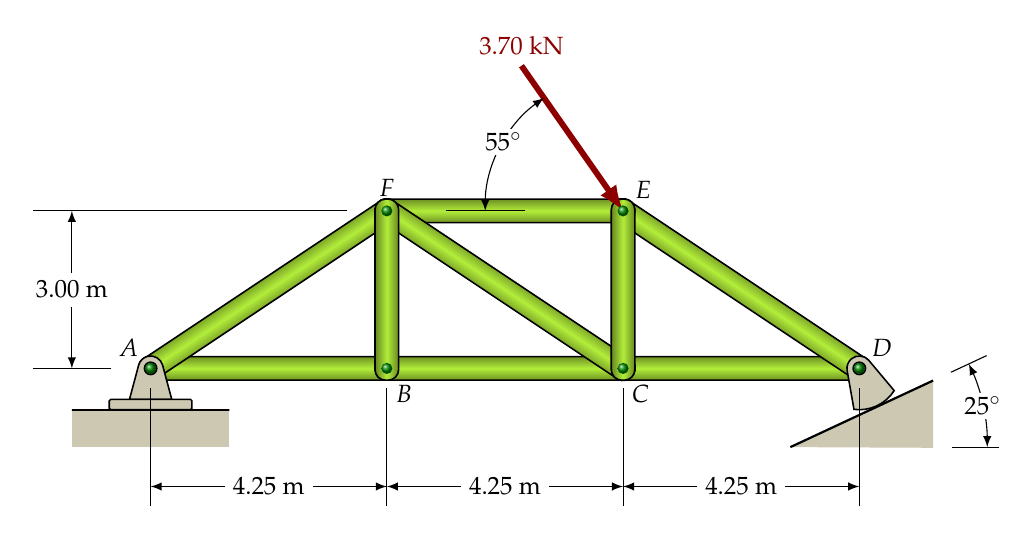
\begin{tikzpicture}[scale=\scale]
	\def\thickness{thick}
	% \def\stroke{black}
	\def\hi{.15}
	\def\radii{\hi}
	\def\extend{\hi}
	\small

	\coordinate (A) at (0, 0);
	\coordinate (B) at (3, 0);
	\coordinate (C) at (6, 0);
	\coordinate (D) at (9, 0);
	\coordinate (E) at (6, 2);
	\coordinate (F) at (3, 2);
	\coordinate (AA) at ($ (A)+(0,-0.5) $);

	% \gettikzxy{(AA)}{\aax}{\aay}	

	\Meme{A}{B}{OliveDrab4}{OliveDrab2}{black}{0.3}{0.135}{0.2}
	\Meme{B}{C}{OliveDrab4}{OliveDrab2}{black}{0.3}{0.135}{0.2}
	\Meme{C}{D}{OliveDrab4}{OliveDrab2}{black}{0.3}{0.135}{0.2}
	\Meme{E}{D}{OliveDrab4}{OliveDrab2}{black}{0.3}{0.135}{0.2}
	\Meme{E}{F}{OliveDrab4}{OliveDrab2}{black}{0.3}{0.135}{0.2}
	\Meme{A}{F}{OliveDrab4}{OliveDrab2}{black}{0.3}{0.135}{0.2}
	\Meme{C}{F}{OliveDrab4}{OliveDrab2}{black}{0.3}{0.135}{0.2}
	\Meme{B}{F}{OliveDrab4}{OliveDrab2}{black}{0.3}{0.135}{0.2}
	\Meme{C}{E}{OliveDrab4}{OliveDrab2}{black}{0.3}{0.135}{0.2}
	
	\fill[Cornsilk3] ($ (A)-(1,0.525) $) rectangle ($ (A)+(1,-1) $);
	\draw[thick] ($ (A)-(1,0.525) $) rectangle ($ (A)+(1,-0.525) $);
	\fill[Cornsilk3] ($ (D)+(-0.875,-1) $) -- ++(25:2) -- +(-90:0.854) -- cycle;
	\draw[thick] ($ (D)+(-0.875,-1) $) -- ++(25:2);

	\PC{A}{Cornsilk3}{black}{0.525}{0.2}
	\Rocker[25]{D}{Cornsilk3}{black}{0.525}{0.2}
	

	\draw ($ (A)+(0,-0.25) $) -- +(0,-1.5);
	\draw ($ (B)+(0,-0.25) $) -- +(0,-1.5);
	\draw ($ (C)+(0,-0.25) $) -- +(0,-1.5);
	\draw ($ (D)+(0,-0.25) $) -- +(0,-1.5);

	\draw[line width=0.75mm, statsMaroon, latex-] (E) -- +(125:2.25) node[above] {$3.70$ kN};
	\draw ($ (E)+(-1.25,0) $)  -- ($ (E)+(-2.25,0) $);
	\draw[latex-latex] ($ (E)+(-1.75,0) $)  arc (180:125:1.75);
	\path  ($ (E)+(150:1.75) $) node[fill=white, inner sep=0.5mm] {\small $55^\circ$};

	\draw ($ (A)-(0.5, 0) $) -- ($ (A)-(1.5, 0) $);
	\draw ($ (F)-(0.5, 0) $) -- ($ (F)-(4.5, 0) $);
	\draw[ latex-latex] ($ (A)-(1, 0) $) -- node[fill=white]{$3.00\text{ m}$}($ (F)-(4, 0) $);

	\draw[ latex-latex] ([yshift=-1.5cm]A) -- node[fill=white]{$4.25\text{ m}$}([yshift=-1.5cm]B);
	\draw[ latex-latex] ([yshift=-1.5cm]B) -- node[fill=white]{$4.25\text{ m}$}([yshift=-1.5cm]C);
	\draw[ latex-latex] ([yshift=-1.5cm]C) -- node[fill=white]{$4.25\text{ m}$}([yshift=-1.5cm]D);

	 \draw ($ (D)+(-0.875,-1)+(25:2.25) $) -- +(25:0.5);
	\draw ($ (D)+(-0.875,-1)+(0:2.05) $) -- +(0:0.6);
	 \draw[latex-latex] ($ (D)+(-0.875,-1)+(0:2.5) $)  arc (0:25:2.5);
	 \path  ($ (D)+(-0.875,-1)+(12:2.5) $) node[fill=white, inner sep=0.5mm] {\small $25^\circ$};

	\shade[ball color=Green4] (A) circle (2pt) node[above left, outer sep=0.5mm] {$A$};
	\shade[ball color=Green4] (B) circle (2pt) node[below right, yshift=-1mm] {$B$};
	\shade[ball color=Green4] (C) circle (2pt) node[below right, yshift=-1mm] {$C$};
	\shade[ball color=Green4] (D) circle (2pt) node[above right, outer sep=0.5mm] {$D$};
	\shade[ball color=Green4] (E) circle (2pt) node[above right, outer sep=0.5mm] {$E$};
	\shade[ball color=Green4] (F) circle (2pt) node[above, outer sep=0.75mm] {$F$};

\end{tikzpicture}

			\cmini[0.8]{
				\centering
				Determine the reactions at $A$ and $D$.
			}
		\end{myexer}
	\end{textblock*}

\end{frame}


%%%%%%%%%%%%%%%%%%%%%%%%%%%%%%%%%%%%%%%%%%%%%%%%%%%%%%%%%%%%%%%%%%%%%%%%%%%%%%%
\begin{frame}
	\begin{textblock*}{1\textwidth}(1cm, 0.25cm)

		\begin{myexer}{}{}
			\def\scale{0.475}
			\centering
			\begin{center}
	\tikz[scale=\scale]{
		\small
		\coordinate (A) at (0,0);
		\coordinate (B) at (4,0);
		\coordinate (C) at (7,0);
		\coordinate (D) at (8,0);
		\coordinate (E) at (8,6);
		\coordinate (F) at (9,0);

		\draw (A) circle (2pt);
		\draw (B) circle (2pt);
		\draw (C) circle (2pt);
		\draw (D) circle (2pt);
		\draw (E) circle (2pt);

		\fill[fill=white] (-2,-4) rectangle (10,8.5);
		\def\hi{0.375}
		\def\twohi{2*\hi}
		\def\threehi{3*\hi}
		\def\innerr{\hi}
		\def\outerr{3*\hi}
		\def\inneroffset{2*\hi}
		\def\outeroffset{\hi}


		\Meme{A}{F}{Tan4}{Tan2}{black}{1}{0.25}{0.5}
		% \pgfoonew \beam =new beam(A, F,Tan3,Tan4, 0.5, 0.5, 0.5)
		\fill[mucus] ($ (A)+(-1,-2) $) rectangle ($ (A)+(-2,2) $);
		\draw[thick, mucus!50!black] ($ (A)+(-1,-2) $) -- ($ (A)+(-1,2) $);
		\PC[-90]{A}{mucus!50}{black}{1}{0.125};

		\draw[saitMaroon, line width=1mm] ($ (D)+(0.5, 0)$) -- ++(0,6)arc(0:150:0.5) -- (B);

		\fill[mucus] ($ (E)+(-2,1) $) rectangle ($ (E)+(2,2) $);
		\draw[thick, mucus!50!black] ($ (E)+(-2,1) $) -- +(4,0);
		 \Pulley[180]{E}{mucus!50}{black}{1}{0.125}

		\draw[-latex, line width=0.75 mm, saitBlue] (C) -- +(0, -3.5) node[left,saitDeepBlue] {\large $22.0\text{ kN}$};

		\shadedraw[ball color=mucus] (A) circle (1.5mm);
		\shadedraw[ball color=mucus] (B) circle (1.5mm);
		\shadedraw[ball color=mucus] (C) circle (1.5mm);
		\shadedraw[ball color=mucus] ($(D)+(0.5,0)$) circle (1.5mm);
		\shadedraw[ball color=mucus] ($(E)$) circle (1.5mm);

		\draw ($ (D)+(0.5,-.75) $) -- +(0, -1.5);
		\draw ($ (B)+(0,-.75) $) -- +(0, -1.5);
		\draw ($ (A)+(0,-.75) $) -- +(0, -1.5);
		%
		\draw[latex-latex] ($ (A)+(0,-1.5) $) -- node[fill=white] {$4.00\;\text{m}$}($ (B)+(0,-1.5) $);
		\draw[latex-latex] ($ (B)+(0,-1.5) $) -- node[fill=white] {$3.00\;\text{m}$}($ (C)+(0,-1.5) $);
		\draw[latex-latex] ($ (C)+(0,-1.5) $) -- ($ (D)+(0.5,-1.5) $);

		\node[right, fill=white,outer sep= 1mm, inner sep=1mm] at ($ (C)+(0, -2) $) {$ 1.50\text{ m}$};

		\draw[latex-latex] ($ (B)+(2,0) $)arc(0:60:2);
		\draw ($ (B)+(1.5,0) $)-- +(1,0);
		\node[fill=white, inner sep=0.5mm] at ($ (B)+(30:2.125) $) {$60\deg$};



	}
\end{center}

			\cmini[0.8]{
				\centering
				Determine the reactions at the pinned connection and the tension in the cable.
			}
		\end{myexer}
	\end{textblock*}

\end{frame}

%%%%%%%%%%%%%%%%%%%%%%%%%%%%%%%%%%%%%%%%%%%%%%%%%%%%%%%%%%%%%%%%%%%%%%%%%%%%%%%
\begin{frame}
	\begin{textblock*}{1\textwidth}(1cm, 0.25cm)

		\begin{myexam}{}{}
			\def\scale{1}
			\centering
			% !TEX root = ../../Beamer/06EquilibriumOfRigidBodies/06ERB.tex

\tikz[scale=\scale]{
	\coordinate (O) at (0,0);
	\coordinate (OO) at (0,0.175);
	\coordinate (A) at ($(O)+(35:3)$);
	\coordinate (B) at ($(O)+(65:3)$);
	\coordinate (C) at ($(O)+(90:3)$);
	\coordinate (D) at ($(O)+(115:3)$);
	\coordinate (E) at ($(O)+(145:3)$);
	\coordinate (top) at ($(C)+(0,1)$);

  \gettikzxy{(A)}{\Ax}{\Ay};
  \gettikzxy{(B)}{\Bx}{\By};
  \gettikzxy{(C)}{\Cx}{\Cy};
  \gettikzxy{(D)}{\Dx}{\Dy};
  \gettikzxy{(E)}{\Ex}{\Ey};
  \gettikzxy{(top)}{\tx}{\ty};

	\filldraw[rounded corners=4pt, fill=Cornsilk3] (OO)-- ++(158:4)-- ++(0,-2)-- ++(7.4175,0)-- +(0,2) -- cycle;
	\filldraw[fill=Cornsilk3]($(A)+(35:0.25)$)arc(35:145:3.25)arc(145:325:0.25)arc(145:35:2.75)arc(215:395:0.25);
	\Roller[-22]{E}{DarkOliveGreen4}{black}{0.5}{0.125};
	\PC[22]{A}{DarkOliveGreen4}{black}{0.51}{0.125};
  \footnotesize
  \draw[very thick, statsMaroon, -Latex] (B)-- +(0,-1.2)node[below, black]{\scriptsize $8.00\,$kN};
  \draw[very thick, statsMaroon, -Latex] (C)-- +(0,-1.475)node[below, black]{\scriptsize $10.0\,$kN};
  \draw[very thick, statsMaroon, -Latex] (D)-- +(0,-1.2)node[below, black]{\scriptsize $12.0\,$kN};
  \draw[very thick, statsMaroon, -Latex] (D)-- +(-1, 0)node[yshift=0.25cm,xshift=0.375cm, black]{\scriptsize$5.00\,$kN};

  \filldraw[ball color=DarkOliveGreen4, thin] (B) circle (0.875mm);
  \filldraw[ball color=DarkOliveGreen4, thin] (C) circle (0.875mm);
  \filldraw[ball color=DarkOliveGreen4, thin] (D) circle (0.875mm);

  \draw[thin, gray] ($(A)+(0,0.7)$) -- (\Ax,\ty);
  \draw[thin, gray] ($(B)+(0,0.5)$) -- (\Bx,\ty);
  \draw[thin, gray] ($(C)+(0,0.45)$) -- (\Cx,\ty);
  \draw[thin, gray] ($(D)+(0,0.5)$) -- (\Dx,\ty);
  \draw[thin, gray] ($(E)+(0,0.6)$) -- (\Ex,\ty);
  \draw[thin, gray] ($(D)+(-1.125,0)$) -- (\Ex-0.75cm,\Dy);
  \draw[thin, gray] ($(E)+(-.375,0)$) -- (\Ex-0.75cm,\Ey);


  \def\dimy{\ty-0.25cm}
  \draw[latex-latex] (\Ex,\dimy)--node[fill=white,inner sep=0.15mm]{\scriptsize $2.50\,$m}(\Dx,\dimy);
  \draw[latex-latex] (\Dx,\dimy)--node[fill=white,inner sep=0.15mm]{\scriptsize $2.50\,$m}(\Cx,\dimy);
  \draw[latex-latex] (\Cx,\dimy)--node[fill=white,inner sep=0.15mm]{\scriptsize $2.50\,$m}(\Bx,\dimy);
  \draw[latex-latex] (\Bx,\dimy)--node[fill=white,inner sep=0.15mm]{\scriptsize $2.50\,$m}(\Ax,\dimy);
  \draw[latex-latex] (\Ex-0.5cm,\Dy)--node[fill=white,inner sep=0.15mm]{\scriptsize $2.10\,$m}(\Ex-0.5cm,\Ey);
}

			\cmini[0.8]{

				The roller and the pinned connection are on slopes inclined at $21\deg$ to the horizontal; they are both at the same elevation.\parm
				Determine the reaction at each connection. Indicate direction by measuring counter-clockwise from the positive $x$-axis.
			}
		\end{myexam}
	\end{textblock*}

\end{frame}

%%%%%%%%%%%%%%%%%%%%%%%%%%%%%%%%%%%%%%%%%%%%%%%%%%%%%%%%%%%%%%%%%%%%%%%%%%%%%%%%
\begin{frame}{}
	\begin{myexam}{}{}
		\def\scale{0.55}
		
\tikz[scale=\scale]{
	\small
	\coordinate (A) at (0,0);
	\coordinate (B) at (8,0);
	\coordinate (C) at (8,4);
	\coordinate (D) at (11,4);
	\coordinate (E) at (5,0);
	\coordinate (F) at (8,2);

	\draw (B) circle (2pt);
	\draw (C) circle (2pt);

	\fill[fill=white] (-3,-2.5) rectangle (13,5.25);
	\def\hi{0.375}
	\def\twohi{2*\hi}
	\def\threehi{3*\hi}
	\def\innerr{\hi}
	% \def\outerr{3*\hi}
	\def\inneroffset{2*\hi}
	\def\outeroffset{\hi}

	\Ronly{D}{mucus}{black}{0.6}{0.25}

	\draw[fill=Cornsilk4!50, draw=black, thick] ($ (A)+(0,\hi) $) -- ($ (B)+(-\twohi,\hi) $) arc(-90:0:\hi) -- ($ (C)+(-\hi,-\twohi) $) arc(180:90:\threehi) -- ($ (D)+(0,\hi) $) arc(90:-90:\hi) -- ($ (C)+(\twohi,-\hi) $)arc(90:180:\hi) -- ($ (B)+(\hi,\twohi) $)arc(0:-90:\threehi) -- ($ (A)+(0,-\hi) $)arc (270:90:\hi);
	\shadedraw[ball color=mucus, black, thick] (D) circle (2mm);
	\PC{A}{mucus}{black}{1}{0.25}

	\fill[mucus] ($ (A)+(-2,-1) $) rectangle ($ (A)+(2,-1.65) $);
	\fill[mucus] ($ (D)+(-1.5,-.6) $) rectangle ($ (D)+(2,-1.25) $);
	\fill[mucus] ($ (D)+(-1.5,.6) $) rectangle ($ (D)+(2,1.25) $);
	\draw[thick, mucus!50!black] ($ (A)+(-2,-1) $) -- ($ (A)+(2,-1) $);
	\draw[thick, mucus!50!black] ($ (D)+(-1.5,.6) $) -- ($ (D)+(2,0.6) $);
	\draw[thick, mucus!50!black] ($ (D)+(-1.5,-.6) $) -- ($ (D)+(2,-0.6) $);

	\draw ($ (D)+(0,-1) $) -- +(0, -5.5);
	\draw ($ (B)+(0,-0.5) $) -- +(0, -2);
	\draw ($ (E)+(0,-0.5) $) -- +(0, -2);
	\draw ($ (A)+(0,-0.5) $) -- +(0, -2);
	\draw ($ (D)+(-2,0) $) -- +(-3.25, 0);
	\draw ($ (B)+(-0.5,0) $) -- +(-2, 0);
	\draw ($ (E)+(-2.75,0) $) -- ($ (E)+(-1.75,0) $);
	\draw[latex-latex] ($ (E)+(125:2.25) $)arc(125:180:2.25);
	\node at ($ (E)+(153:2.25) $) [fill=white]{$55^\circ$};

	\draw[latex-latex] ($ (A)+(0,-2) $) -- node[fill=white] {$2.50\;\text{m}$}($ (E)+(0,-2) $);
	\draw[latex-latex] ($ (E)+(0,-2) $) -- node[fill=white] {$1.50\;\text{m}$}($ (B)+(0,-2) $);
	\draw[latex-latex] ($ (B)+(0,-2) $) -- node[fill=white] {$1.50\;\text{m}$}($ (D)+(0,-6) $);
	\draw[latex-latex] ($ (C)+(-1.75,0) $) -- node[fill=white] {$2.00\;\text{m}$}($ (B)+(-1.75,0) $);

	\draw[latex-, ultra thick, statsMaroon] (E) -- +(125:2.75) node[above,black] {$1.24\;\text{kN}$};
	\Couple{F}{statsMaroon}{0.75}{.75}
  % \draw[-Straight Barb, ultra thick, statsMaroon] ($ (F)+(-70:0.875) $)arc(-70:289:0.875) node[below right, fill=white, inner sep=1mm, outer sep=1mm] {$\bm{ 3.75}\;\text{\bfseries{kN}}\bm\cdot\text{\bfseries m}$};
	\node[xshift=1cm, yshift=-0.5cm] at (F) {$1.75\,\mathsf{kN\cd m} $};

	\node[above left, outer sep = 1mm] at (A) {\large $A$};
	\node[right, outer sep = 3mm] at (D) {\large $B$};

}

		\parb\centering
		The roller at $B$ is in a smooth slot.\par
		Determine the reactions at $A$ and $B$.
		
	\end{myexam}
\end{frame}

%%%%%%%%%%%%%%%%%%%%%%%%%%%%%%%%%%%%%%%%%%%%%%%%%%%%%%%%%%%%%%%%%%%%%%%%%%%%%%
\begin{frame}
	\begin{textblock*}{1\textwidth}(1cm, 0.25cm)

		\begin{myexam}{}{}
			\def\scale{0.75}
			\centering
			% !TEX root = ../../Beamer/06EquilibriumOfRigidBodies/06ERBforDT.tex



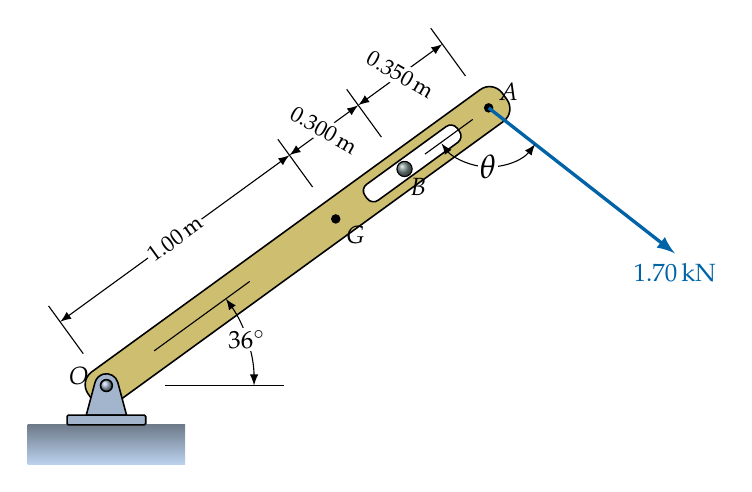
\begin{tikzpicture}[scale=\scale]
	\def\thickness{0.25}
	\def\stroke{black}
	\def\hi{.25}
	\def\radii{\hi*0.5}
	\def\extend{\hi}

	\coordinate (A) at (0, 0);
	\coordinate (B) at ($(A)+(36:6)$);
	\coordinate (G) at ($(A)!0.6!(B)$);
	\coordinate (P) at ($(A)+(15:4)$);

	\coordinate (D) at ($(G)!0.25!(B)$);
	\coordinate (E) at ($(G)!0.75!(B)$);
	\coordinate (C) at ($(D)!0.4!(E)$);

	\small

	\fill[top color = LightSteelBlue4, bottom color=LightSteelBlue2] ($(A)+(-1,-0.5)$) rectangle +(2,-0.5);
	\Meme{A}{B}{LightGoldenrod3}{LightGoldenrod3}{black}{0.5}{0.2}{.2}
	% \pgfoonew \AB=new rr(A,B,LightGoldenrod3,black, 0.125)
	\def\hi{0.125}
	\def\extend{\hi}
	\def\radii{\hi}
	\Meme{D}{E}{white}{white}{black}{0.25}{0.1}{.2}
	% \pgfoonew \DE=new rr(D,E,white,black, 0.125)
	\PC{A}{LightSteelBlue3}{black}{0.5}{0.2}

	\node[yshift=1.25mm, xshift=-3.5mm , inner sep=2mm] at (A) {$O$};
	\filldraw (G) circle (1.5pt) node[yshift=-2mm, xshift=2.5mm , inner sep=2mm] {$G$};
	\filldraw (B) circle (1.5pt) node[yshift=2mm, xshift=2.5mm , inner sep=2mm] {$A$};
	\filldraw[ball color=LightCyan4] (C) circle (2.75pt) node[yshift=-2.25mm, xshift=1.75mm ] { $B$};
	\draw[-latex, very thick, saitDeepBlue] (B) -- +(-38:3)node[below]{$1.70\,$kN};

	\draw ($(B)+(216:0.25)$) -- +(216:0.75);
	\draw[latex-latex] ($(B)+(-38:0.75)$)arc[start angle=322, end angle=217, radius=0.75]node[midway, fill=white, inner sep=.2mm]{\large $\theta$};



	\draw ($(A)+(0:0.75)$) -- +(0:1.5);
	\draw ($(A)+(36:0.75)$) -- +(36:1.5);
	\draw[latex-latex] ($(A)+(-0:1.875)$)arc[start angle=0, end angle=36, radius=1.875]node[midway, fill=white, inner sep=.3mm]{\small $36\deg$};

	\draw ($(A)+(126:0.5)$) -- +(126:0.75);
	\draw ($(G)+(126:0.5)$) -- +(126:0.75);
	\draw ($(B)+(126:0.5)$) -- +(126:0.75);
	\draw ($(C)+(126:0.5)$) -- +(126:0.75);
	\footnotesize
	\draw[latex-latex]($(A)+(126:1)$) -- node[fill=white, inner sep=0.25mm, sloped]{$1.00\,$m}($(G)+(126:1)$);
	\draw[latex-latex]($(G)+(126:1)$) -- node[fill=white, inner sep=0.5mm, rotate=-30]{$0.300\,$m}($(C)+(126:1)$);
	\draw[latex-latex]($(C)+(126:1)$) -- node[fill=white, inner sep=0.5mm, rotate=-30]{$0.350\,$m}($(B)+(126:1)$);

\end{tikzpicture}

			\parm
			
			$55$-kg bar $AB$ has its centre of gravity at $G$. It is supported by a pinned connection at $A$ and a smooth peg at $C$. A cable is attached at $B$ and has a tensile force of $1.70\,$kN. The direction of the cable varies between $\theta=60\deg$ and $\theta=135\deg$. \parm

			What is the maximum reaction at $P$? \par Determine the reaction at $A$ for this maximum reaction at $P$.
			
		\end{myexam}
	\end{textblock*}
\end{frame}

%%%%%%%%%%%%%%%%%%%%%%%%%%%%%%%%%%%%%%%%%%%%%%%%%%%%%%%%%%%%%%%%%%%%%%%%%%%%%%%

\begin{frame}{}
	\begin{myexam}{}{}
		\cmini[0.95]{
			\def\scale{0.8}
			\centering
			\tikz[scale=\scale]{
	\coordinate (A) at (0,-0.25);
	\coordinate (B) at (7,-0.25);
	\coordinate (C) at (0,2.5);
	\coordinate (D) at (3,1);
	\coordinate (E) at (7,1);
	\coordinate (base) at (0,0.025);
	\coordinate (Aleft) at ($(A)+(-0.5,0)$);

	\DL{C}{D}{base}{DarkOliveGreen2}{black}{6}{0.35}{5}
	\DL{D}{E}{base}{DarkOliveGreen2}{black}{8}{0.35}{5}	

	\fill[AntiqueWhite3] ($ (A)+(0,3.5) $) rectangle ($ (A)+(-1,-1.5) $);
	\draw[thick] ($ (A)+(0,3.5) $) -- +(0, -5);
	\Meme{A}{B}{AntiqueWhite4}{AntiqueWhite2}{black}{0.5}{0}{.2}	

	\fill (A) circle (1.5pt) node [left, xshift=-1mm] {\Large $A$};
	\node at (B) [right,xshift=1mm] {\Large $B$};
	\node at ($ (C) + (1.1,0.1)  $) {$4.00\text{ kN/m}$};
	\node at ($ (D) + (1.5,0.2)  $) {$1.50\text{ kN/m}$};

	\draw ($ (D)+(0,-1.75) $) -- +(0,-0.5);
	\draw ($ (E)+(0,-1.75) $) -- +(0,-0.5);

	\draw[Latex-Latex] ([yshift=-0.75cm]A) -- node[fill=white, inner sep=0.5mm] {$3.00$ m} ([yshift=-2cm]D);
	\draw[Latex-Latex] ([yshift=-2cm]D) -- node[fill=white, inner sep=0.5mm] {$4.00$ m} ([yshift=-0.75cm]B);

}

			
			Beam $AB$ has a fixed support at $A$. (Fixed supports offer resistance to rotation in the form of a reacting couple at $A$; clearly, without this, equilibrium would not be possible.)\parm

			Determine the reaction and the reacting moment at $A$.		
		}	
	\end{myexam}
\end{frame}

%%%%%%%%%%%%%%%%%%%%%%%%%%%%%%%%%%%%%%%%%%%%%%%%%%%%%%%%%%%%%%%%%%%%%%%%%%%%%%%%
%%%%%%%%%%%%%%%%%%%%%%%%%%%%%%%%%%%%%%%%%%%%%%%%%%%%%%%%%%%%%%%%%%%%%%%%%%%%%%%

\begin{frame}{Fixed Supports}
	\begin{myexer}{}{}
		\centering\def\scale{0.75}
		\tikz[scale=\scale]{
	\coordinate (A) at (0,-0.25);
	\coordinate (Aleft) at (-0.5,-0.25);
	\coordinate (B) at (6,-0.25);
	\coordinate (C) at (0,2.75);
	\coordinate (D) at (6,1);
	\coordinate (E) at (3.5,-0.25);
	\coordinate (base) at (0,0.025);
	\coordinate (couple) at (2.75,-0.25);


	% \def\scale{1}
	\def\hi{.25}
	\small

	\DL{C}{D}{base}{LightSkyBlue}{DarkBlue}{9}{0.25}{5}
	\fill[Honeydew3] ($ (A)+(0,4) $) rectangle ($ (A)+(-1,-2) $);
	\draw[thick] ($ (A)+(0,4) $) -- +(0, -6);
	\Meme{A}{B}{Honeydew4}{Honeydew1}{black}{0.5}{0}{0.5}	

	\node[above right] at (C) {$ 2.50\text{ kN/m}$};
	\node[above] at ($ (D)+(0,0.25) $) {$ 1.00\text{ kN/m}$};

	\draw (6,-0.75) -- +(0,-1.5);
	\draw[latex-latex] (0,-1.625) -- node[fill=white] {\small $1.00$ m} (6,-1.625);

	\draw ($ (B)+(.5,0) $) -- +(1.25,0);
	\node at ($ (B)+(15:1.25) $) {\small $35\deg$};

	\Couple[0]{couple}{statsMaroon}{0.5}{0.5}
	\node[xshift=0.75cm, yshift=-0.5cm, statsMaroon] at (couple) {$ 5.25\,\mathsf{kN\cd m}$};

	\draw[-latex, ultra thick, statsMaroon] (B)  -- +(35:2.25) node[right] {$ 4.25\text{ kN}$};


\fill (A) circle (1.5pt) node [left,outer sep=1mm] {\large $A$};
\node at (B) [below right,outer sep=0.5mm] {\large $B$};

}

		\parb
		Determine the reaction and reacting moment at $A$.
		
	\end{myexer}
\end{frame}


%%%%%%%%%%%%%%%%%%%%%%%%%%%%%%%%%%%%%%%%%%%%%%%%%%%%%%%%%%%%%%%%%%%%%%%%%%%%%%%%
\begin{frame}{}
	\begin{myexam}{}{}
		\centering
		\def\scale{1}
		

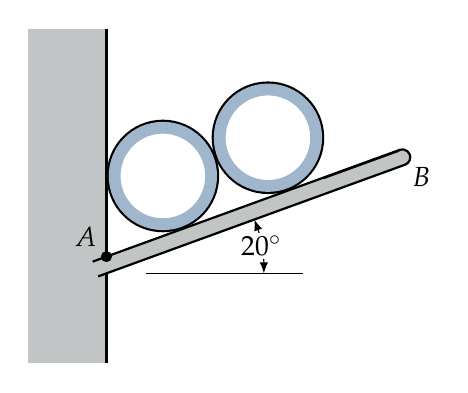
\begin{tikzpicture}[scale=\scale]
	\coordinate (A) at (0,0);
	\coordinate (B) at ($ (A)+(20:4) $);
	\coordinate (AA) at ($ (A)+(0, 0.1067) $);
	\coordinate (C) at ($ (A)+(0, 0.1067)+ (55:1.25) $);
	\coordinate (D) at ($ (C)+(20:1.42) $);

	
	\fill[Azure4!50] ($ (A)+(0,3) $) rectangle +(-1,-4.25);
	\draw[thick] ($ (A)+(0,3) $) --($ (A)+(0,-1.25) $);

	\draw[line width=0.2cm, Azure4!50, line cap=round] ($ (A)+(200:0.15) $) -- (B);

	% \Meme{A}{B}{SteelBlue3}{SteelBlue3}{SteelBlue3}{0.3}{0}{0}
	\draw[thick] ($ (A)+(110:0.1)+(200:0.15) $)--+(20:4.15);
	\draw[thick] ($ (A)+(-70:0.1)+(200:0.15) $)--+(20:4.15)arc(-70:130:0.1)--+(200:1);

	\fill (AA)circle(2pt)node[above left] {$ A $};
	\node[below right] at  (B) {$ B $};

	\draw[line width= 0.15cm] (C) circle (0.64cm);
	\draw[line width= 0.15cm,SlateGray3] (C) circle (0.6125cm);
	\draw[line width= 0.15cm] (D) circle (0.64cm);
	\draw[line width= 0.15cm,SlateGray3] (D) circle (0.6125cm);

	\draw ($ (A)-(0,0.1067)+(0.5,0) $) -- +(2,0);
	\draw[latex-latex] ($ (A)-(0,0.1067)+(2,0) $) arc(0:20:2)node[midway, fill=white, inner sep=0.4mm]{$ 20\deg $};


\end{tikzpicture}

		\parb
		Pipe racks ($AB$, and two hidden behind it) support two smooth Schedule 40 pipes, with an outside diameter of $508\,\text{mm}$, as shown. The pipes are $10\,\text{m}$ in length with a mass of $78.5\,\text{kg/m}$, Each rack supports one-third of the weight of each pipe.\parm 
		Determine the reaction at the fixed connection $A$.
		
	\end{myexam}
\end{frame}
%%%%%%%%%%%%%%%%%%%%%%%%%%%%%%%%%%%%%%%%%%%%%%%%%%%%%%%%%%%%%%%%%%%%%%%%%%%%%%%%
%%%%%%%%%%%%%%%%%%%%%%%%%%%%%%%%%%%%%%%%%%%%%%%%%%%%%%%%%%%%%%%%%%%%%%%%%%%%%%%%
\begin{frame}{}
	\begin{myexer}{}{}
		\centering
		\def\scale{0.65}
		% !TEX root = ../../Beamer/06EquilibriumOfRigidBodies/06ERB.tex


\tikz[scale=\scale]{
	\coordinate (A) at (0,-0.25);
	\coordinate (B) at (7,-0.25);
	\coordinate (C) at (0,2.5);
	\coordinate (D) at (3,1);
	\coordinate (E) at (7,1);
	\coordinate (base) at (0,0.025);
	\coordinate (Aleft) at ($(A)+(-0.5,0)$);

	% \def\scale{1}
	\def\hi{.25}
	\def\radii{0}
	\def\extend{0}



	\def\scale{1}
	\fill[LightSkyBlue!50!] (C) -- (D) -- (E) -- ($ (B)+(0,0.25)$) -- (base) -- cycle;
	% \DLOne{C}{D}{base}{LightSkyBlue}{DarkBlue}{6}{0.25}
	% \DLOne{D}{E}{base}{LightSkyBlue}{DarkBlue}{8}{0.25}
	\pgfoonew \AB=new beam(Aleft,B,AntiqueWhite2,AntiqueWhite4, 0.25, 0,0.5)



	\draw (0,-0.75) -- +(0,-0.5);
	\draw (1,-0.75) -- +(0,-0.5);
	\draw (3.5,-0.75) -- +(0,-0.5);

	\draw[Latex-Latex] (0,-1) -- node[ yshift=-.25cm] {\small $1.00$ m} (1,-1);
	\draw[Latex-Latex] (1,-1) -- node[fill=white, outer sep=0.5mm] {\small $2.50$ m} (3.5,-1);


	% \fill[mucus!75!white] ($ (A)+(0,3.5) $) rectangle ($ (A)+(-1,-1.5) $);
	% \draw[mucus!75!black, very thick] ($ (A)+(0,3.5) $) -- +(0, -5);

	\draw[Latex-, ultra thick, saitBlue] (3.5,0)  -- +(0,2.5) node[above, black] {$ 10.50\text{ kN}$};
	\draw[Latex-, ultra thick, saitBlue] (1,0)  -- +(0,1) node[above, black] {$ 3.75\text{ kN}$};


	\node at (B) [right] {\Large $B$};

	\draw[ultra thick, -Latex, saitRed] ($ (A)+(-60:0.5) $)arc(-60:60:0.5)-- +(140:0.1)node[right, yshift=0.1cm] {$\bm M_a$};
	\draw[ultra thick, -Latex, saitRed] (A)-- +(1,0)node[right] {$\bm R_{A_x}$};
	\draw[ultra thick, -Latex, saitRed] (A)-- +(0,1)node[right] {$\bm R_{A_y}$};

	\fill (A) circle (1.5pt) node [left] {\Large $A$};
}

		\parb
		A section of smooth pipe, centred at $O$, has a diameter of $457\,\text{mm}$ and a mass of $186\,\text{kg}$. It is secured by vertical structural member $AB$, hinged with a pinned connection at $A$ and held in place by chain $BC$. \parm Determine the tension in the chain, and the reaction at $A$.		
		
	\end{myexer}
\end{frame}
%%%%%%%%%%%%%%%%%%%%%%%%%%%%%%%%%%%%%%%%%%%%%%%%%%%%%%%%%%%%%%%%%%%%%%%%%%%%%%%%
%%%%%%%%%%%%%%%%%%%%%%%%%%%%%%%%%%%%%%%%%%%%%%%%%%%%%%%%%%%%%%%%%%%%%%%%%%%%%%%%
\begin{frame}{}
	\begin{myexam}{}{}
		\centering
		\def\scale{0.5}
		\tikz[scale=\scale]{
  \coordinate (A) at (0,0);
  \coordinate (C) at (1,0);
  \coordinate (D) at (2.2,0);
  \coordinate (E) at (5.6,0);
  \coordinate (B) at (8,0);

  \fill[DarkOliveGreen4] ($(A)+(-2,0)$) rectangle ($ (B)+(2,-3.75) $);
  
  \node[below left, Cornsilk2] at (A) {$ A $};
  \node[below right, Cornsilk2] at (B) {$ B $};

  \fill[SlateGray3] ($ (C)-(0.25,0) $) rectangle ($ (C)+(0.25,4) $);
  \draw[SlateGray4, very thick] ($ (C)+(-0.25,0) $) rectangle ($ (C)+(-0.25,4) $);
  \draw[SlateGray4, very thick] ($ (C)+(0.25,0) $) rectangle ($ (C)+(0.25,4) $);
  \fill[SlateGray3] ($ (D)-(0.25,0) $) rectangle ($ (D)+(0.25,4) $);
  \draw[SlateGray4, very thick] ($ (D)+(-0.25,0) $) rectangle ($ (D)+(-0.25,4) $);
  \draw[SlateGray4, very thick] ($ (D)+(0.25,0) $) rectangle ($ (D)+(0.25,4) $);
  \fill[SlateGray3] ($ (E)-(0.25,0) $) rectangle ($ (E)+(0.25,4) $);
  \draw[SlateGray4, very thick] ($ (E)+(-0.25,0) $) rectangle ($ (E)+(-0.25,4) $);
  \draw[SlateGray4, very thick] ($ (E)+(0.25,0) $) rectangle ($ (E)+(0.25,4) $);

  \draw[very thick, latex-] ($ (C)+(0,4) $) --+ (0,2)node[above]{\small$ 200\,\textsf{kN} $};
  \draw[very thick, latex-] ($ (D)+(0,4) $) --+ (0,1.4)node[above]{\small$ 140\,\textsf{kN} $};
  \draw[very thick, latex-] ($ (E)+(0,4) $) --+ (0,1.6)node[above]{\small$ 160\,\textsf{kN} $};

  \draw[thin, gray] ($ (A)+(0,0.5) $) -- ($ (A)+(0,5.5) $);
  \draw[thin, gray] ($ (B)+(0,0.5) $) -- ($ (B)+(0,5.5) $);

  \draw[latex-latex] ($ (A)+(0,4.75) $) -- ($ (C)+(0,4.75) $) node[midway, fill=white, yshift=0.157cm,inner sep=0mm] {\scriptsize $ 1\,\textsf{m}$};
  \draw[latex-latex] ($ (C)+(0,4.75) $) -- ($ (D)+(0,4.75) $) node[midway, fill=white, yshift=0.157cm,inner sep=0mm] {\scriptsize $ 1.2\,\textsf{m}$};
  \draw[latex-latex] ($ (D)+(0,4.75) $) -- ($ (E)+(0,4.75) $) node[midway, fill=white, yshift=0.157cm,inner sep=0mm] {\scriptsize $ 3.4\,\textsf{m}$};
  \draw[latex-latex] ($ (E)+(0,4.75) $) -- ($ (B)+(0,4.75) $) node[midway, fill=white, yshift=0.157cm,inner sep=0mm] {\scriptsize $ 2.4\,\textsf{m}$};

  \begin{scope}[yshift=-0.75cm]
    \coordinate (TL) at (0,1);
    \coordinate (TR) at (8,2);
    \coordinate (base) at (0,0);
    \DLdown[180]{TL}{TR}{base}{DarkOliveGreen4}{Cornsilk2}{10}{0.4}{5};
  \end{scope}

  \filldraw[fill=Cornsilk2] (A) rectangle ($ (B)+(0,-0.75) $);
  \draw [thick] ($ (A)+(-2,0) $) -- ($ (B)+(2,0) $);
  \node[Cornsilk2] at (-0.5,-3) {$ \omega_1 $};
  \node[Cornsilk2] at (8.5,-2) {$ \omega_2 $};


}
		\pars
		\cmini[0.7]{
			\centering
			Soil exerts a trapezoidal distributed load on the bottom of the footing $AB$. \parm Determine the values of $\omega_1$ and $\omega_2$ that support the column loadings in static equilibrium.		
		}
	\end{myexam}
\end{frame}
%%%%%%%%%%%%%%%%%%%%%%%%%%%%%%%%%%%%%%%%%%%%%%%%%%%%%%%%%%%%%%%%%%%%%%%%%%%%%%%%


%%%%%%%%%%%%%%%%%%%%%%%%%%%%%%%%%%%%%%%%%%%%%%%%%%%%%%%%%%%%%%%%%%%%%%%%%%%%%%%%
\begin{frame}{Notes:}
	\cmini[0.9]{
		\begin{enumerate}
			\item  For a body in equilibrium, $\Sigma M=0$ for moments summed about {\bfseries any} point in the plane containing the body.\pars
			\item We have used all the three equations of statics to solve for three unknowns. It would also have been possible to solve using $\Sigma M=0$ three times by choosing appropriate points about which to take moments. There are occasions when it is more convenient to sum moments two or three times, rather than summing components. (We will see this when using the Method of Sections to analyze forces in truss members.)\pars
			\item Since there are only three equations for statics, we can only solve a system for three unknowns. Frequently, two unknowns come from a pinned connection and the third from a cable, roller or some other connection whose reaction direction is known. (Alternatively, we can solve for a fixed connection, which has three unknowns.)\pars
			\item Generally, we start by taking moments about the pinned connection - so that we don't need to consider the moments of the pinned connection unknowns. Then, the moment equation will immediately give a solution for the third unknown, e.g., for a connection with a known force direction.
		\end{enumerate}

	}
\end{frame}

%%%%%%%%%%%%%%%%%%%%%%%%%%%%%%%%%%%%%%%%%%%%%%%%%%%%%%%%%%%%%%%%%%%%%%%%%%%%%%

\begin{frame}{Two-Force Members}

	\mini[0.4]{
		For a member with only two external forces acting upon it to be in equilibrium:\parm
		\begin{itemize}
			\item Both forces must share the same line of action
			\item Both forces must have the same magnitude
			\item The forces must have opposite directions
		\end{itemize}
		\parm
		Then, $\Sigma F_x=0 $, $\Sigma F_y=0 $ {\bfseries and} there is no tendency for the member to rotate.
		\parm
		Strut connections and cables are two-force members!

	}
	\hfill
	\mini[0.5]{
		\def\scale{0.75}
		\tcb{
			
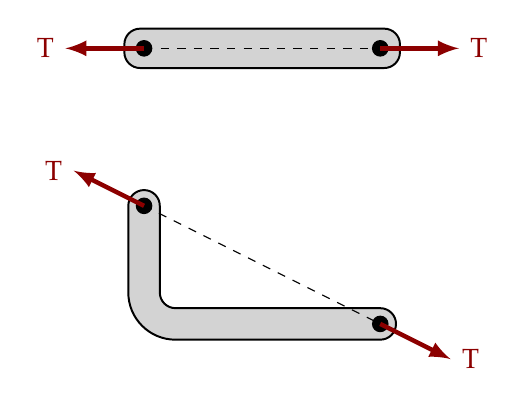
\begin{tikzpicture}[scale=\scale]
			\def\hi{.2}

			\coordinate (T1) at (1.5, 0);
			\coordinate (T2) at (4.5, 0);
			\coordinate (Ba) at (1.5,-2);
			\coordinate (Bb) at (1.5, -3.5);
			\coordinate (Bc) at (4.5, -3.5);

			\Meme{T1}{T2}{LightGray}{LightGray}{black}{0.5}{0.2}{0.25}

			\fill[black] (T1) circle (3pt);
			\fill[black] (T2) circle (3pt);
			\gettikzxy{(Ba)}{\Bax}{\Bay}
			\gettikzxy{(Bb)}{\Bbx}{\Bby}
			\gettikzxy{(Bc)}{\Bcx}{\Bcy}

			\filldraw[line width=0.25mm, fill=LightGray, draw=black] (\Bax-\hi cm, \Bay) -- (\Bbx-\hi cm, \Bby+2*\hi cm) arc(180:270:3*\hi) -- (\Bcx, \Bcy-\hi cm) arc(-90:90:\hi)--(\Bbx+2*\hi cm, \Bby+\hi cm) arc(270:180:\hi)--(\Bax+\hi cm, \Bay) arc(0:180:\hi);

			\draw[dashed] (T1) -- (T2);
			% \draw[dashed] (C1) -- (C2);
			\draw[dashed] (Ba) -- (Bc);

			\fill[black] (Ba) circle (3pt);
			\fill[black] (Bc) circle (3pt);

			\draw[ultra thick, saitMaroon, -latex] (T1) -- +(-1, 0) node[left] {T};
			\draw[ultra thick, saitMaroon, -latex] (T2) -- +(1, 0) node[right] {T};
			\draw[ultra thick, saitMaroon, -latex] (Ba) -- +(153.44:1) node[left] {T};
			\draw[ultra thick, saitMaroon, -latex] (Bc) -- +(-26.57:1) node[right] {T};
%
		\end{tikzpicture}

		}
	}

\end{frame}

%%%%%%%%%%%%%%%%%%%%%%%%%%%%%%%%%%%%%%%%%%%%%%%%%%%%%%%%%%%%%%%%%%%%%%%%%%%%%%%%
\begin{frame}{Straight Two-Force Members}
	\def\scale{0.75}
	In straight two-force members, the lines of action of the forces are along the member.\lb The forces shown here are {\bfseries external} forces applied to the member.
	\begin{center}
		\tcb{
			%%%%%%%%%%%%%%%%%%%%%%% TRUSS %%%%%%%%%%%%%%%%%%%%%%%%%%%%%%%%%%%%%%%%%%%%%%%%%%%%%%%%%%%%%%%%%%%%%
% !TEX root = ../../04MoJ/04MoJ.tex


%%%%%%%%%%%%%%%%%%%%%%% TRUSS %%%%%%%%%%%%%%%%%%%%%%%%%%%%%%%%%%%%%%%%%%%%%%%%%%%%%%%%%%%%%%%%%%%%%


%%%%%%%%%%%%%%%%%%%%%%% TRUSS %%%%%%%%%%%%%%%%%%%%%%%%%%%%%%%%%%%%%%%%%%%%%%%%%%%%%%%%%%%%%%%%%%%%%
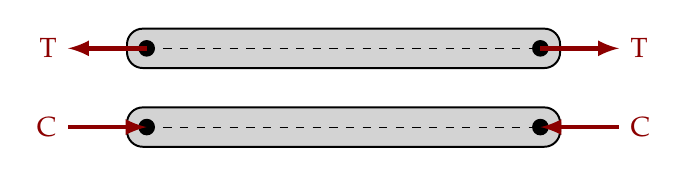
\begin{tikzpicture}[scale=\scale]
			
			\coordinate (T1) at (1.5, 0);
			\coordinate (T2) at (6.5, 0);
			\coordinate (C1) at (1.5,-1);
			\coordinate (C2) at (6.5, -1);

			\Meme{T1}{T2}{LightGray}{LightGray}{black}{0.5}{0.2}{0.25}
			\Meme{C1}{C2}{LightGray}{LightGray}{black}{0.5}{0.2}{0.25}

			\fill[black] (T1) circle (3pt);
			\fill[black] (T2) circle (3pt);
			\fill[black] (C1) circle (3pt);
			\fill[black] (C2) circle (3pt);

			\draw[dashed] (T1) -- (T2);
			\draw[dashed] (C1) -- (C2);

			\draw[ultra thick, saitMaroon, -latex] (T1) -- +(-1, 0) node[left] {T};
			\draw[ultra thick, saitMaroon, -latex] (T2) -- +(1, 0) node[right] {T};
			\draw[ultra thick, saitMaroon, latex-] (C1) -- +(-1, 0) node[left] {C};
			\draw[ultra thick, saitMaroon, latex-] (C2) -- +(1, 0) node[right] {C};
			
		\end{tikzpicture}

		}
	\end{center}

	\uncover<2->{
		These external forces generate corresponding {\bfseries internal} forces which can be examined by `cutting' a section through the member:
		\begin{center}
			\tcb{
				%%%%%%%%%%%%%%%%%%%%%%% TRUSS %%%%%%%%%%%%%%%%%%%%%%%%%%%%%%%%%%%%%%%%%%%%%%%%%%%%%%%%%%%%%%%%%%%%%
% !TEX root = ../../04MoJ/04MoJ.tex


%%%%%%%%%%%%%%%%%%%%%%% TRUSS %%%%%%%%%%%%%%%%%%%%%%%%%%%%%%%%%%%%%%%%%%%%%%%%%%%%%%%%%%%%%%%%%%%%%


%%%%%%%%%%%%%%%%%%%%%%% TRUSS %%%%%%%%%%%%%%%%%%%%%%%%%%%%%%%%%%%%%%%%%%%%%%%%%%%%%%%%%%%%%%%%%%%%%
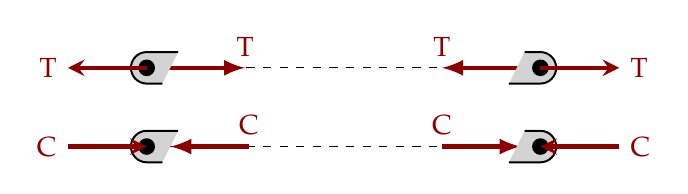
\begin{tikzpicture}[scale=\scale]
	\def\thickness{thick}
	\def\stroke{Khaki4}
	\def\hi{.2}
	\def\radii{\hi}
	\def\extend{\hi}

	% \fill[white] (0,0) rectangle (5.5,1);

	\coordinate (Ta) at (1.5, 0);
	\coordinate (Tb) at (6.5, 0);
	\coordinate (Ca) at (1.5,-1);
	\coordinate (Cb) at (6.5, -1);

	\gettikzxy{(Ta)}{\tax}{\tay}
	\gettikzxy{(Tb)}{\tbx}{\tby}
	\gettikzxy{(Ca)}{\cax}{\cay}
	\gettikzxy{(Cb)}{\cbx}{\cby}

	\draw[dashed] (Ta) -- (Tb);
	\draw[dashed] (Ca) -- (Cb);

	\draw[ultra thick, saitMaroon, -latex] ($ (Ta)+(0.25,0) $) -- +(1, 0) node[above] {T};
	\draw[ultra thick, saitMaroon, -latex] ($ (Tb)+(-0.25,0) $) -- +(-1, 0) node[above] {T};
	\draw[ultra thick, saitMaroon, latex-] ($ (Ca)+(0.3,0) $) -- +(1, 0) node[above] {C};
	\draw[ultra thick, saitMaroon, latex-] ($ (Cb)+(-0.25,0) $) -- +(-1, 0) node[above] {C};

	\filldraw[line width=0.25mm, fill=LightGray] (\tax+2*\hi cm,\tay+\hi cm) -- (\tax, \tay+\hi cm) arc(90:270:\hi)--(\tax+\hi cm, \tay-\hi cm);
	\filldraw[line width=0.25mm, fill=LightGray] (\tbx-\hi cm,\hi) -- (\tbx, \hi) arc(90:-90:\hi)--(\tbx-2*\hi cm, \tby-\hi cm);

	\filldraw[line width=0.25mm, fill=LightGray] (\cax+2*\hi cm,\cay+\hi cm) -- (\cax, \cay+\hi cm) arc(90:270:\hi)--(\cax+\hi cm, \cay-\hi cm);
	\filldraw[line width=0.25mm, fill=LightGray] (\cbx-\hi cm,\cby+\hi cm) -- (\cbx , \cby+\hi cm) arc(90:-90:\hi)--(\cbx-2*\hi cm, \cby-\hi cm);

	\fill[black] (Ta) circle (3pt);
	\fill[black] (Tb) circle (3pt);
	\fill[black] (Ca) circle (3pt);
	\fill[black] (Cb) circle (3pt);



	\draw[ultra thick, saitMaroon, ->, >=stealth] (Ta) -- +(-1, 0) node[left] {T};
	\draw[ultra thick, saitMaroon, ->, >=stealth] (Tb) -- +(1, 0) node[right] {T};
	\draw[ultra thick, saitMaroon, <-, >=stealth] (Ca) -- +(-1, 0) node[left] {C};
	\draw[ultra thick, saitMaroon, <-, >=stealth] (Cb) -- +(1, 0) node[right] {C};

%
\end{tikzpicture}

			}
		\end{center}
	}
\end{frame}

%%%%%%%%%%%%%%%%%%%%%%%%%%%%%%%%%%%%%%%%%%%%%%%%%%%%%%%%%%%%%%%%%%%%%%%%%%%%%%%%%%%%%%%%%%%%%%%%%%%%

\begin{frame}{External and Internal Forces}
	\def\scale{0.65}
	\cmini[1]{
		It is important to distinguish between external and internal forces.

		When a two-force member is in tension, external forces pull {\bfseries away} from the member (attempting to make the member longer). The opposite is true for compression.
		\parb\centering
		
		\begin{statsbox}[width=0.65\linewidth]{External Forces}
			\centering
			%%%%%%%%%%%%%%%%%%%%%%% TRUSS %%%%%%%%%%%%%%%%%%%%%%%%%%%%%%%%%%%%%%%%%%%%%%%%%%%%%%%%%%%%%%%%%%%%%
% !TEX root = ../../04MoJ/04MoJ.tex


%%%%%%%%%%%%%%%%%%%%%%% TRUSS %%%%%%%%%%%%%%%%%%%%%%%%%%%%%%%%%%%%%%%%%%%%%%%%%%%%%%%%%%%%%%%%%%%%%


%%%%%%%%%%%%%%%%%%%%%%% TRUSS %%%%%%%%%%%%%%%%%%%%%%%%%%%%%%%%%%%%%%%%%%%%%%%%%%%%%%%%%%%%%%%%%%%%%
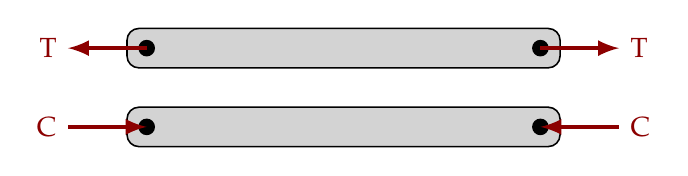
\begin{tikzpicture}[scale=\scale]
	
	\coordinate (T1) at (1.5, 0);
	\coordinate (T2) at (6.5, 0);
	\coordinate (C1) at (1.5,-1);
	\coordinate (C2) at (6.5, -1);

	\Meme{T1}{T2}{LightGray}{LightGray}{black}{0.5}{0.15}{0.2}
	\Meme{C1}{C2}{LightGray}{LightGray}{black}{0.5}{0.15}{0.2}
	
	\fill[black] (T1) circle (3pt);
	\fill[black] (T2) circle (3pt);
	\fill[black] (C1) circle (3pt);
	\fill[black] (C2) circle (3pt);


	\draw[ultra thick, saitMaroon, -latex] (T1) -- +(-1, 0) node[left] {T};
	\draw[ultra thick, saitMaroon, -latex] (T2) -- +(1, 0) node[right] {T};
	\draw[ultra thick, saitMaroon, latex-] (C1) -- +(-1, 0) node[left] {C};
	\draw[ultra thick, saitMaroon, latex-] (C2) -- +(1, 0) node[right] {C};
%
\end{tikzpicture}

		\end{statsbox}

		\parb
	
		\begin{statsbox}[width=0.65\linewidth]{Internal Forces} 
			\centering
			%%%%%%%%%%%%%%%%%%%%%%% TRUSS %%%%%%%%%%%%%%%%%%%%%%%%%%%%%%%%%%%%%%%%%%%%%%%%%%%%%%%%%%%%%%%%%%%%%
% !TEX root = ../../04MoJ/04MoJ.tex


%%%%%%%%%%%%%%%%%%%%%%% TRUSS %%%%%%%%%%%%%%%%%%%%%%%%%%%%%%%%%%%%%%%%%%%%%%%%%%%%%%%%%%%%%%%%%%%%%


%%%%%%%%%%%%%%%%%%%%%%% TRUSS %%%%%%%%%%%%%%%%%%%%%%%%%%%%%%%%%%%%%%%%%%%%%%%%%%%%%%%%%%%%%%%%%%%%%
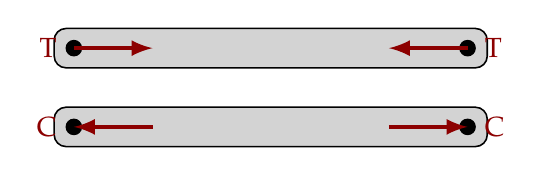
\begin{tikzpicture}[scale=\scale]
	
	\coordinate (T1) at (1.5, 0);
	\coordinate (T2) at (6.5, 0);
	\coordinate (C1) at (1.5,-1);
	\coordinate (C2) at (6.5, -1);

	\Meme{T1}{T2}{LightGray}{LightGray}{black}{0.5}{0.15}{0.2}
	\Meme{C1}{C2}{LightGray}{LightGray}{black}{0.5}{0.15}{0.2}

	\fill[black] (T1) circle (3pt);
	\fill[black] (T2) circle (3pt);
	\fill[black] (C1) circle (3pt);
	\fill[black] (C2) circle (3pt);

	\draw[ultra thick, saitMaroon, latex-] ($(T1)+(1,0)$) -- +(-1, 0) node[left, xshift=-0.75mm] {T};
	\draw[ultra thick, saitMaroon, latex-] ($(T2)+(-1,0)$) -- +(1, 0) node[right, xshift=0.75mm] {T};
	\draw[ultra thick, saitMaroon, -latex] ($(C1)+(1,0)$) -- +(-1, 0) node[left, xshift=-0.75mm] {C};
	\draw[ultra thick, saitMaroon, -latex] ($(C2)+(-1,0)$) -- +(1, 0) node[right, xshift=0.75mm] {C};
%
\end{tikzpicture}

		\end{statsbox}
	
	}

\end{frame}

%%%%%%%%%%%%%%%%%%%%%%%%%%%%%%%%%%%%%%%%%%%%%%%%%%%%%%%%%%%%%%%%%%%%%%%%%%%%%%%%%%%%%%%%%%%%%%%%%%%%%%%%%%%%%%%%%%%%%%%%%%%%%%

\begin{frame}{External and Internal Forces}
	\def\scale{0.65}
	\cmini[1]{
		Initially, the direction of internal forces may seem counter-intuitive.
\begin{center}
			\begin{statsbox}[width=0.65\linewidth]{Internal Forces}
				\centering
				%%%%%%%%%%%%%%%%%%%%%%% TRUSS %%%%%%%%%%%%%%%%%%%%%%%%%%%%%%%%%%%%%%%%%%%%%%%%%%%%%%%%%%%%%%%%%%%%%
% !TEX root = ../../04MoJ/04MoJ.tex


%%%%%%%%%%%%%%%%%%%%%%% TRUSS %%%%%%%%%%%%%%%%%%%%%%%%%%%%%%%%%%%%%%%%%%%%%%%%%%%%%%%%%%%%%%%%%%%%%


%%%%%%%%%%%%%%%%%%%%%%% TRUSS %%%%%%%%%%%%%%%%%%%%%%%%%%%%%%%%%%%%%%%%%%%%%%%%%%%%%%%%%%%%%%%%%%%%%
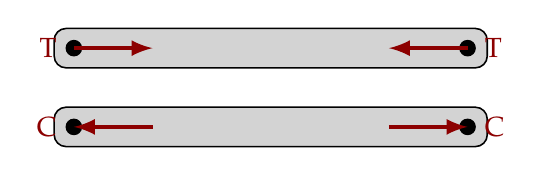
\begin{tikzpicture}[scale=\scale]
	
	\coordinate (T1) at (1.5, 0);
	\coordinate (T2) at (6.5, 0);
	\coordinate (C1) at (1.5,-1);
	\coordinate (C2) at (6.5, -1);

	\Meme{T1}{T2}{LightGray}{LightGray}{black}{0.5}{0.15}{0.2}
	\Meme{C1}{C2}{LightGray}{LightGray}{black}{0.5}{0.15}{0.2}

	\fill[black] (T1) circle (3pt);
	\fill[black] (T2) circle (3pt);
	\fill[black] (C1) circle (3pt);
	\fill[black] (C2) circle (3pt);

	\draw[ultra thick, saitMaroon, latex-] ($(T1)+(1,0)$) -- +(-1, 0) node[left, xshift=-0.75mm] {T};
	\draw[ultra thick, saitMaroon, latex-] ($(T2)+(-1,0)$) -- +(1, 0) node[right, xshift=0.75mm] {T};
	\draw[ultra thick, saitMaroon, -latex] ($(C1)+(1,0)$) -- +(-1, 0) node[left, xshift=-0.75mm] {C};
	\draw[ultra thick, saitMaroon, -latex] ($(C2)+(-1,0)$) -- +(1, 0) node[right, xshift=0.75mm] {C};
%
\end{tikzpicture}

			\end{statsbox}
		\end{center}
	}
	 Why do internal forces pull towards each other when the member is in tension? It is because external forces are trying to `stretch' the member and the internal forces are opposing this stretch, maintaining the length of the member.\parm

	 Similarly, when a straight two-force member is in compression, internal forces in the member `push back' against the external compression.\parm

	 Furthermore, at the ends of the two-force members, external and internal forces must be equal and opposite to each other to maintain equilibrium.

\end{frame}

%%%%%%%%%%%%%%%%%%%%%%%%%%%%%%%%%%%%%%%%%%%%%%%%%%%%%%%%%%%%%%%%%%%%%%%%%%%%%%%%%%%%%%%%%%


	\begin{frame}{A Second Look at Strut/Link Connections}

		\def\scale{0.5}
		\begin{textblock*}{1\textwidth}(1.5 cm, 1.5 cm)
					% !TEX root = ../../Beamer/06EquilibriumOfRigidBodies/06ERB.tex

\tikz[scale=\scale, line cap = round]{
	\def\xshift{8}
	\def\yshift{4}
	\def\xxshift{4}
	\def\rotate{-30}
	\coordinate (O) at (0,0);
	\coordinate (A) at ($(O)+(-105:6)$);
	\coordinate (OO) at ($(O)+(\xshift,0)$);
	\coordinate (AA) at ($(A)+(\xshift,0)$);
	\coordinate (OOO) at ($(OO)+(\xxshift,-\yshift)$);
	\coordinate (AAA) at ($(AA)+(\xxshift,-\yshift)$);

	% \def\thickness{thick}
	% \def\stroke{black}
	% \def\hi{.3}
	% \def\radii{\hi}
	% \def\extend{\hi}

	\PC{A}{gray!75!white}{black}{1}{0.125}
	\begin{scope}[transform canvas={rotate=\rotate}]
		\filldraw [top color=gray, bottom color=gray, middle color=gray!50, thick]($(O)+(5,0.5)$)  -- +(-5,0)arc(90:270:0.5)-- +(4.5,0);
	\end{scope}
	\node[xshift=-0.375cm, yshift=0.375cm] at (O) {\large $A$};
	\node[xshift=-0.375cm, yshift=0.125cm] at (A) {\large $B$};
	\node[xshift=3cm, yshift=2.25cm] at (A) {\large $C$};
	
	\Meme{O}{A}{gray!50}{gray!50}{black}{0.75}{0.2}{.25}

	\draw[line width=1.875mm, black, line cap = round]($(O)+(-105:0.5)$)-- ($(A)+(75:0.5)$);
	\draw[line width=1.5mm, saitDeepBlue!70, line cap = round]($(O)+(-105:0.5)$)-- ($(A)+(75:0.5)$);

	
	\filldraw[ball color=gray] (O) circle (2mm);
	\filldraw[ball color=gray] (A) circle (2mm);
	\fill[top color=mucus, bottom color=mucus!25] ($(A)+(-3,-0.5)$) rectangle +(6,-1);
	\draw[thick] ($(A)+(-3,-0.50)$)-- +(6,0);

	\only<1>{
	\draw[ultra thick, -latex, statsMaroon](O) -- ($(O)!0.5!(A) $)node[right,xshift=1mm]{$\bm R$};
	}
	\only<2>{
	\draw[ultra thick, latex-, statsMaroon](O) -- ($(O)!0.5!(A) $)node[right,xshift=1mm]{$\bm R$};
	}


	\begin{scope}[scale=0.75]
		\uncover<1,3>{
			\node[xshift=0.5cm, yshift=0.4cm] at (OO) {Strut in Tension};
			\begin{scope}
				\filldraw [fill=gray!50, draw=gray, thick, rotate around = {\rotate:(\xshift, 0 )}]($(OO)+(5,0.5)$)  -- +(-5,0)arc(90:270:0.5)-- +(4.5,0);
			\end{scope}
			\fill[gray] (OO) circle (2mm);
			\draw[ultra thick, -latex, saitMaroon](OO) -- ($(OO)!0.5!(AA) $)node[below]{$\bm R$};
		}
		\uncover<2-3>{
			\node[xshift=0.5cm, yshift=0.4cm] at (OOO) {Strut in Compression};
			\begin{scope}[xshift=\xxshift, yshift=-\yshift]
				\begin{scope}
					\filldraw [fill=gray!50, draw=gray, thick, rotate around = {\rotate:(\xshift, 0 )}]($(OOO)+(5,0.5)$)  -- +(-5,0)arc(90:270:0.5)-- +(4.5,0);
				\end{scope}
				\fill[gray] (OOO) circle (2mm);
				\draw[ultra thick, latex-, saitMaroon](OOO) -- ($(OOO)!0.5!(AAA) $)node[below]{$\bm R$};
			\end{scope}
		}
	\end{scope}
}

		\end{textblock*}

		\begin{textblock*}{0.8\textwidth}(2cm, 7cm)
			\only<1>{
			When strut $AB$ is in {\bfseries tension} (due to forces in $AC$), it `pulls' back against $AC$ to maintain equilibrium.
			}
			\only<2>{
			When strut $AB$ is in {\bfseries compression} (due to forces in $AC$), it `pushes' against $AC$ to maintain equilibrium.
			}
			\uncover<3>{
			Frequently, we don't know in advance whether $AB$ is in tension or in compression. In that case, we draw the force acting on $AC$ in tension (i.e., arrow directed {\bfseries away} from $AC$). If our calculations determine that $R$ is negative, then $AB$ is in compression.
			}
		\end{textblock*}

	\end{frame}

	%%%%%%%%%%%%%%%%%%%%%%%%%%%%%%%%%%%%%%%%%%%%%%%%%%%%%%%%%%%%%%%%%%%%%%%%%%%%%%%
\begin{frame}

		\begin{myexam}{}{}
			\def\scale{0.65}
			\centering
			% !TEX root = ../../Beamer/06EquilibriumOfRigidBodies/06ERB.tex

\makeatletter
\providecommand{\gettikzxy}[3]{%
	\tikz@scan@one@point\pgfutil@firstofone#1\relax
	\edef#2{\the\pgf@x}%
	\edef#3{\the\pgf@y}%
}
\makeatother

\begin{tikzpicture}[scale=\scale]
	

	\coordinate (A) at (0, 0);
	\coordinate (B) at (3, 0);
	\coordinate (C) at (7, 0);
	\coordinate (D) at (10, 1.25);
	\coordinate (E) at (10, -3.5);
	\coordinate (F) at (7, -3.5);
	\coordinate (G) at (3, -3.5);

	\fill[left color=mucus, right color=mucus!50] ($ (E)+(0.75,-1.25) $) rectangle ($ (D)+(1.5,2) $);
	\draw[black, line width=0.2mm] ($ (E)+(0.75,-1.25) $) -- ($ (D)+(0.75,2) $);

	\PC[90]{D}{mucus!50}{black}{0.75}{0.2}
	\PC[90]{E}{mucus!50}{black}{0.75}{0.2}

	\gettikzxy{(A)}{\Ax}{\Ay};
	\gettikzxy{(B)}{\Bx}{\By};

	\Meme{A}{B}{LightCyan4}{LightCyan1}{black}{0.35}{0.125}{0.2}
	\Meme{C}{D}{LightCyan4}{LightCyan1}{black}{0.35}{0.125}{0.2}
	\Meme{A}{G}{LightCyan4}{LightCyan1}{black}{0.35}{0.125}{0.2}
	\Meme{F}{G}{LightCyan4}{LightCyan1}{black}{0.35}{0.125}{0.2}
	\Meme{F}{E}{LightCyan4}{LightCyan1}{black}{0.35}{0.125}{0.2}
	\Meme{C}{G}{LightCyan4}{LightCyan1}{black}{0.35}{0.125}{0.2}
	\Meme{C}{E}{LightCyan4}{LightCyan1}{black}{0.35}{0.125}{0.2}
	\Meme{C}{B}{LightCyan4}{LightCyan1}{black}{0.35}{0.125}{0.2}
	\Meme{C}{F}{LightCyan4}{LightCyan1}{black}{0.35}{0.125}{0.2}
	\Meme{B}{G}{LightCyan4}{LightCyan1}{black}{0.35}{0.125}{0.2}

	\gettikzxy{(C)}{\Cx}{\Cy};
	\gettikzxy{(E)}{\Ex}{\Ey};
	\gettikzxy{(D)}{\Dx}{\Dy};

	\draw ($ (A)+(0,0.5) $) -- +(0,2.75);
	\draw ($ (B)+(0,0.5) $) -- +(0,2.75);
	\draw ($ (C)+(0,0.5) $) -- +(0,2.75);
	\draw ($ (D)+(0,0.5) $) -- +(0,1.5);
	\draw ($ (E)+(1,0) $) -- (13, \Ey);
	\draw ($ (C)+(0.75,0) $) -- (13, \Cy);
	\draw ($ (D)+(1,0) $) -- (13, \Dy);

	\draw[line width=0.75mm, black, -latex, saitMaroon] (A) -- +(0,-2.5) node[below, saitMaroon] {\large {$ 30$ kN}};

	\draw[thick, <->, >=stealth] ([yshift=2.5cm]A) -- node[fill=white]{\small $3.00\text{ m}$}([yshift=2.5cm]B);
	\draw[thick, <->, >=stealth] ([yshift=2.5cm]B) -- node[fill=white]{\small $4.00\text{ m}$}([yshift=2.5cm]C);
	\draw[thick, <->, >=stealth] ([yshift=2.5cm]C) -- node[fill=white]{\small $3.00\text{ m}$}([yshift=1.25cm]D);
	\draw[thick, <->, >=stealth] (12.5, \Dy) -- node[fill=white, inner sep=0.5mm]{\small $1.25\text{ m}$}(12.5, \Cy);
	\draw[thick, <->, >=stealth] (12.5, \Cy) -- node[fill=white, inner sep=0.5mm]{\small $3.50\text{ m}$}(12.5, \Ey);

	\filldraw[ball color=LightCyan4, thin] (A) circle (2.5pt) node[above left, inner sep=2mm] {\large $A$};
	\filldraw[ball color=LightCyan4, thin] (B) circle (2.5pt) node[above left, inner sep=2mm] {\large $B$};
	\filldraw[ball color=LightCyan4] (C) circle (2.5pt) node[above left, inner sep=2mm] {\large $C$};
	\filldraw[ball color=LightCyan4] (D) circle (2.5pt) node[above left, inner sep=2mm] {\large $D$};
	\filldraw[ball color=LightCyan4] (E) circle (2.5pt) node[below, inner sep=2mm] {\large $E$};
	\filldraw[ball color=LightCyan4] (F) circle (2.5pt) node[below, inner sep=2mm] {\large $F$};
	\filldraw[ball color=LightCyan4] (G) circle (2.5pt) node[below , inner sep=2mm] {\large $G$};

\end{tikzpicture}

			\cmini[0.85]{
				\centering
				Determine the reactions at $D$ and $E$.\parb
				% \textcolor{saitMaroon}{Note}: There are two pinned connections, but there is a single link between $C$ and $D$ so $CD$ is a {\bfseries two-force member}, so the direction of the reaction at $D$ is in the direction of $CD$ and has only one unknown - its magnitude.
			}
			
		\end{myexam}

\end{frame}

		%%%%%%%%%%%%%%%%%%%%%%%%%%%%%%%%%%%%%%%%%%%%%%%%%%%%%%%%%%%%%%%%%%%%%%%%%%%%%%%
\begin{frame}

		\begin{myexer}{}{}
			\def\scale{0.65}
			\centering
			

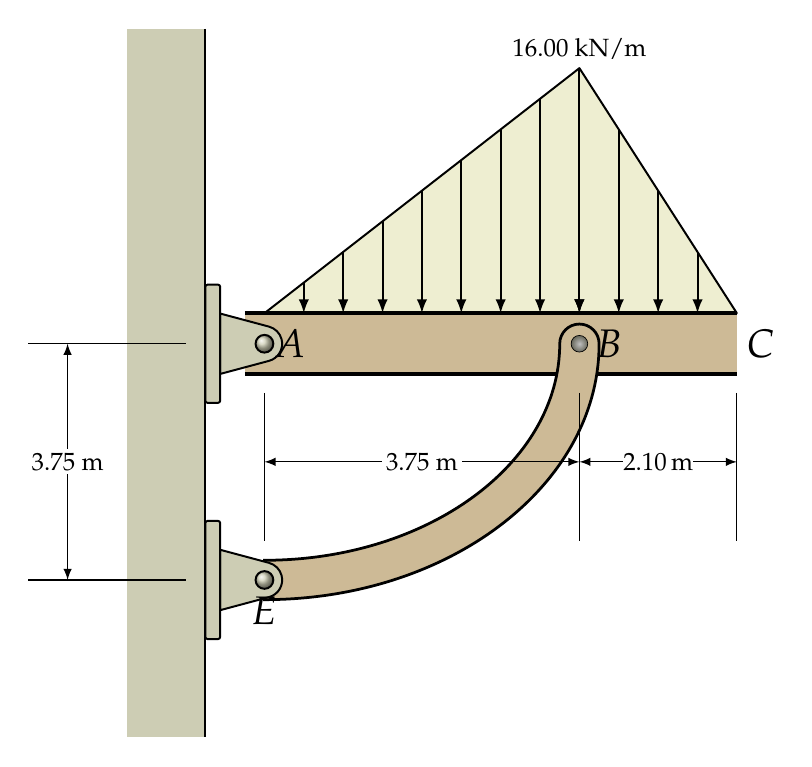
\begin{tikzpicture}[scale=\scale]
	% \def\thickness{thick}
	% \def\stroke{black}
	% \def\radii{0.25}
	% \def\extend{0.25}
	% \def\ldraw{RosyBrown4!50!black}
	% \def\lfill{saitBlue}

	\coordinate (A) at (0, 0);
	\coordinate (AA) at ($(A)+(1.5,2)$);
	\coordinate (B) at (4, 0);
	\coordinate (C) at (6, 0);
	\coordinate (CC) at ($(C)+(0,1.55*0.25)$);
	\coordinate (D) at (4,3.5);
	\coordinate (E) at (0,-3);
	\coordinate (base) at ($(A)+(0,0.3875)$);

	\fill[LightYellow3] ($ (A)+(-0.75,4) $) rectangle ($ (E)+(-1.75,-2) $);
	\draw[black, thick] ($ (A)+(-0.75,4) $) -- +(0, -9);

	\DL{base}{D}{base}{LightYellow2}{black}{8}{0.25}{5}
	\DL{CC}{D}{base}{LightYellow2}{black}{4}{0.25}{5}


	\fill[Wheat3] ($ (A)+(-0.25,-0.3875) $) rectangle ($ (C)+(0,0.3875) $);
	\draw[ultra thick] ($ (A)+(-0.25,-0.3875) $) -- ++(6.25,0);
	\draw[ultra thick] ($ (A)+(-0.25,0.3875) $) -- ++(6.25,0);



	\filldraw [fill=Wheat3, draw=black, line width=0.35mm] (0,-2.75) arc [start angle=-90, end angle=0, x radius=3.75cm, y radius=2.75cm]arc(180:0:0.25) arc[start angle=0, end angle=-90, x radius=4.25cm, y radius=3.25cm] -- cycle;

	\PC[-90]{A}{LightYellow3}{black}{0.75}{0.25}
	\PC[-90]{E}{LightYellow3}{black}{0.75}{0.25}

	\shadedraw[outer color=\ldraw!50!\lfill, inner color=\ldraw!25!white, \ldraw, line width = \lwidth pt] (B) circle (3pt);


	\node at (A) [right] {\Large $A$};
	\node at (B) [right, outer sep=1mm] {\Large $B$};
	\node at (C) [right] {\Large $C$};

	\node at ($ (D)+(0,0.25) $) {\small $16.00$ kN/m};
	\node at (E) [below, outer sep=1mm] {\Large $E$};


	\draw ($ (A)+(-1,0) $) -- +(-2,0);
	\draw ($ (E)+(-1,0) $) -- +(-2,0);
	\draw ($ (A)+(0,-0.625) $) -- +(0,-1.875);
	\draw ($ (B)+(0,-0.625) $) -- +(0,-1.875);
	\draw ($ (C)+(0,-0.625) $) -- +(0,-1.875);
\draw[latex-latex] ([yshift=-1.5cm]A) -- node[fill=white, inner sep=0.5mm] {\small $3.75$ m} ([yshift=-1.5cm]B);
\draw[latex-latex] ([yshift=-1.5cm]B) -- node[fill=white, inner sep=0.mm] {\small $2.10\thinspace$m} ([yshift=-1.5cm]C);
\draw[latex-latex] ([xshift=-2.5cm]A) -- node[fill=white, inner sep=0.5mm] {\small $3.75$ m} ([xshift=-2.5cm]E);


\end{tikzpicture}

			\cmini[0.8]{
				\centering
				Determine the reactions at $A$ and $D$.
			}
			
		\end{myexer}
\end{frame}
%%%%%%%%%%%%%%%%%%%%%%%%%%%%%%%%%%%%%%%%%%%%%%%%%%%%%%%%%%%%%%%%%%%%%%%%%%%%%%%%

%%%%%%%%%%%%%%%%%%%%%%%%%%%%%%%%%%%%%%%%%%%%%%%%%%%%%%%%%%%%%%%%%%%%%%%%%%%%%%%
\begin{frame}
	
%
		\begin{myexer}{}{}
			\def\scale{0.65}
			\centering
			% !TEX root = ../../Beamer/06EquilibriumOfRigidBodies/06ERB.tex

\tikz[scale=\scale]{
	\coordinate (O) at (0,0);
	% \coordinate (OO) at (0,0.175);
	\coordinate (A) at ($(O)+(4,2)$);
	\coordinate (B) at ($(O)+(0,-4.472)$);
	\coordinate (C) at ($(O)+(0:4.472)$);
	\coordinate (D) at ($(O)+(-40:4.472)$);
	\coordinate (E) at ($(O)+(145:3)$);
	\coordinate (top) at ($(C)+(0,1)$);

  \def\radius{4.472}
  \def\hi{0.25}
  \def\outer{\radius+\hi}
  \def\inner{\radius-\hi}

  \gettikzxy{(A)}{\Ax}{\Ay};
  \gettikzxy{(B)}{\Bx}{\By};
  \gettikzxy{(C)}{\Cx}{\Cy};
  \gettikzxy{(D)}{\Dx}{\Dy};
  \gettikzxy{(E)}{\Ex}{\Ey};
  \gettikzxy{(top)}{\tx}{\ty};

  \fill[left color=LightYellow3, right color=LightYellow4] ($(O)+(-0.75,3)$) rectangle ($(B)+(-2,-2)$);
  \draw[LightYellow4!50!black] ($(O)+(-0.75,3)$) -- ($(B)+(-0.75,-2)$);

  \filldraw[fill=SlateGray4!50!SlateGray3] ($(A)+(26.6:\hi)$)arc(26.6:-90:\outer)arc(270:90:\hi)arc(-90:26.6:\inner)arc(206.6:26.6:\hi);
  \filldraw[rounded corners=1.5mm, fill=SlateGray3] ($(O)+(-\hi,-\hi)$)-- (-\hi,\Ay+\hi cm)-- (\Ax+\hi cm,\Ay+\hi cm)--(\Ax+\hi cm,\Ay-\hi cm)--(\hi+1,\Ay-\hi cm)--(\hi,\Ay-\hi cm-1cm)--(\hi,-\hi)--cycle;
  \PC[-90]{O}{LightYellow3}{black}{0.75}{0.125};
	\PC[-90]{B}{LightYellow3}{black}{0.75}{0.125};
  \footnotesize
  \draw[ultra thick, saitMaroon, -Latex] (C)-- +(0:2)node[right, black]{ $8.00\,$kN};
  \draw[ultra thick, saitMaroon, -Latex] (D)-- +(-40:2)node[right, black]{ $8.00\,$kN};
\draw[dashed] ($(O)+(26.6:0.25)$)--($(A)+(206.6:0.25)$);
\draw[dashed] ($(O)+(0:0.25)$)--($(C)+(0:0.25)$);
\draw[dashed] ($(O)+(-40:0.25)$)--($(D)+(1400:0.25)$);

\draw ($(O)+(-80:4.472)$)arc(-80:-50:4.472);
\normalsize
  \filldraw[ball color=LightYellow3, thin] (A) circle (1.25mm) node[xshift=3mm, yshift=3mm]{$C$};
  \filldraw[ball color=LightYellow3, thin] (B) circle (1.25mm)node[yshift=4mm]{$B$};
  \filldraw[ball color=LightYellow3, thin] (O) circle (1.25mm)node[yshift=-4mm]{$A$};
  \filldraw[ball color=LightYellow3, thin] (C) circle (1.25mm);
  \filldraw[ball color=LightYellow3, thin] (D) circle (1.25mm);
\draw[semithick,-Latex] (O)-- node[fill=white,inner sep=0.4mm]{\footnotesize $R=1.25\,$m}+(-65:4.472);

\draw[latex-latex] ($(O)+(0:2.25)$)arc(0:26.6:2.25)node[midway,fill=white, inner sep=0.2mm]{\footnotesize $27.0\deg$};
\draw[latex-latex] ($(O)+(0:2.25)$)arc(0:-40:2.25)node[midway,fill=white, inner sep=0.2mm]{\footnotesize $42.0\deg$};

}

			\cmini[0.8]{
				\centering
				Member $CD$ is a circular arc with centre at $A$.\pars
				Determine the reactions at $A$ and $B$.
			}
		
		\end{myexer}
	
\end{frame}

%%%%%%%%%%%%%%%%%%%%%%%%%%%%%%%%%%%%%%%%%%%%%%%%%%%%%%%%%%%%%%%%%%%%%%%%%%%%%%%
\begin{frame}
	
%
		\begin{myexam}{}{}
			\def\scale{0.825}
			\centering
			% !TEX root = ../../00temp/downOne/prospectives.tex

\tikz[scale=\scale,xscale=-1]{
	\def\r{0.35};
	% for 10deg
	\def\sin{0.17365}
	\def\cos{0.98481}
	\def\hyp{1.5}

	\scriptsize

	\fill [top color=Honeydew4,bottom color=Honeydew3] (-3,-1.075) rectangle (7,-2);
	\draw (-3,-1.075) -- +(7,0);

	\coordinate (O) at (1,0);
	\coordinate (R) at (4.975,0.125);
	\coordinate (F) at ($(R)+(150:2.475)$);
	\coordinate (FF) at ($(O)+(2.25,0)$);

	% hydraulic
	\begin{scope}[transform canvas={rotate around={-36:(O)}}]
		\shadedraw[top color=Azure4,bottom color=Azure4, middle color=white] ($ (O)+(0.125,-0.05) $) rectangle +(2.5,0.1);
		\shadedraw[top color=Azure4,bottom color=Azure4, middle color=white] ($ (O)+(-0.125,-0.075) $) rectangle +(1.125,0.15);		
	\end{scope}

	\begin{scope}
		%draw back gate
		\begin{scope}[rotate around={-30:(R)}]
			\filldraw[fill=Honeydew3, draw=black] (5.325,2) circle (0.75mm);
			\filldraw[draw=black,fill=Honeydew3, rotate around={30:(5.325,2)}] (5.24,2) rectangle +(-0.0625,-1.875);
		\end{scope}
		% truck cargo
		\begin{scope}[rotate around={-30:(R)}]
			\coordinate (G) at (2.5,1);
			\filldraw[draw=black,fill=Honeydew3] (0,0)-- ++(0,2.25)-- ++(5.25,0)-- +(0,-2.25)--cycle;
			\fill (G) circle (1.25pt)node[xshift=2.5mm]{\normalsize $G$};
			% \draw ($ (G)+(-90:0.25) $) -- +(-90:1);
			% dimensions
			\draw ($(F)+(0,1.0625)$) -- ++(0,1.625);
			\draw ($(F)+(0,0.125)$) -- ++(0,.6125);
			\draw ($(R)+(0,0.25)$) -- +(0,2.5);
			% \draw ($(G)+(0,0.25)$) -- +(0,1.625);
			% \draw[latex-latex] ($(F)+(0,2.45)$) -- node[fill=white,rotate=30]{$1.65\,$m}($(G)+(0,1.575)$);
			\draw[latex-latex] ($(G)+(0,1.575)$) -- node[fill=white,rotate=30]{$2.50\,$m}($(R)+(0,2.45)$);
			\draw ($(F)+(0.125,0)$) -- ($(R)+(-0.25,0)$);
			\draw ($(G)+(0.125,0)$) -- +(1,0);
			\draw[latex-latex] ($(G)+(0.75,0)$) -- node[fill=Honeydew3, rotate=30]{$1.15\,$m}($(G)+(0.75,-0.875)$);
		\end{scope}
		% \draw (O)--($(O)+(76.5:2.25)$);
	\end{scope}
	% rear pinned connection
	\begin{scope}[scale=.25]
		\filldraw[fill=Honeydew4,draw=black] ($(R)+(\cos*\r,\sin*\r)$)arc(10:170:\r)-- ++(-\sin*\hyp,-\cos*\hyp)-- ++(2*\sin*\hyp+2*\r, 0)-- cycle;		
	\end{scope}
	% hydraulic lower connection
	\begin{scope}[scale=.25]
		\PC{O}{Honeydew4}{black}{1.25}{0.125}
	\end{scope}
	% truck body
	\filldraw[draw=black,fill=Green3] (-0.0625,-0.0625)-- ++(0.65,0)-- ++(0,-0.15)-- ++(0.7,0)-- ++(0,0.15)-- ++(3.45,0)-- ++(0,-0.15)-- ++(0.5,0)-- ++(0,-0.4)-- ++(-0.8,0)arc(0:180:0.55)-- +(-4.5,0)arc(0:180:0.55)-- ++(-0.0625,0)-- ++(0,0.55)-- ++(0.0625,0.0625)-- ++(0.0625,0.325)arc(160:99:0.125)-- ++(8:0.9)-- ++(65:0.6)arc(155:90:0.125)-- ++(0.65,0)arc(90:0:0.125)-- cycle;

	\draw ($(O)+(0.4,0.06)+(35.5:1.375)$) -- ++(216:1.375)-- +(1.375,0);
	\draw[latex-latex] ($(O)+(0.4,0.06)+(0:1.125)$)arc(0:36:1.125)node[midway,fill=white,inner sep=0.25mm]{$36.5\deg$};
	\draw ($(R)+(-0.375,-0.075)+(180:1.5)$) -- ++(0:1.5)-- +(150:1.5);
	\draw[latex-latex] ($(R)+(-0.375,-0.075)+(150:1.25)$)arc(150:180:1.25)node[midway,fill=white,inner sep=0.125mm]{$31.5\deg$};


	\filldraw[fill=Honeydew4,draw=black] (3.89,-0.6) circle (0.475cm);
	\filldraw[fill=white,draw=black] (3.89,-0.6) circle (0.3cm);
	\filldraw[fill=Green3,draw=black] (3.89,-0.6) circle (0.225cm);
	\filldraw[fill=Honeydew4,draw=black] (-1.7125,-0.6)  circle (0.475cm);
	\filldraw[fill=white,draw=black] (-1.7125,-0.6) circle (0.3cm);
	\filldraw[fill=Green3,draw=black] (-1.7125,-0.6) circle (0.225cm);
	\draw[black](-.2,1)-- ++(0,-1.175)arc(0:-90:0.0625)-- ++(-0.6,0)arc(270:225:0.0625)-- ++(135:0.25)arc(225:180:0.0625)-- ++(0,0.5)arc(180:165:0.125)-- ++(69:0.5)arc(161:90:0.0625)-- +(0.595,0)arc(90:0:0.0625);
	\filldraw[fill=white, draw=black](-.26,0.95)-- ++(0,-0.5)-- ++(-0.725,0)arc(270:161:0.0625)-- ++(69:0.45)arc(161:90:0.0625)-- ++(0.5125,0)arc(90:5:0.05);

	\shadedraw[ball color=LightBlue4,draw=black] (R) circle (0.5mm);
	\shadedraw[ball color=LightBlue4,draw=black] (F) circle (0.5mm);
	\shadedraw[ball color=LightBlue4,draw=LightBlue4!50!black] (O) circle (0.5mm);

	\small
	\node[xshift=0.175cm,yshift=0.175cm] at (O) {\bm $A$};
	\node[xshift=0.125cm,yshift=0.175cm] at (F) { \bm $B$};
	\node[xshift=0.125cm,yshift=0.3cm] at (R) {\bm $C$};


}

			\cmini[0.775]{
				\centering
				The bin of a dump-truck is being tipped by hydraulic lift $AB$. ($AB$ can be considered a two-force member.) The bin rotates about a pin at $C$. Determine the force in the lift $AB$ and find the reaction at $C$ if the bin has a mass of $880\,\textsf{kg}$ and $G$ marks its centre of mass.
			}
		
		\end{myexam}
	
\end{frame}

%%%%%%%%%%%%%%%%%%%%%%%%%%%%%%%%%%%%%%%%%%%%%%%%%%%%%%%%%%%%%%%%%%%%%%%%%%%%%%%
\begin{frame}
	
%
		\begin{myexer}{}{}
			\def\scale{0.6}
			\centering
			
\tikz[scale=\scale, line cap=round,decoration={
	markings,% switch on markings
	mark=% actually add a mark
	between positions 0 and 1 step 9pt
	with
	{
		\begin{scope}[scale=0.75]
			\draw[Goldenrod4, line width=0.4mm] (0pt,-2pt) -- ++(4pt,0) arc(-90:90:2pt) -- ++(-4pt,0pt) arc(90:270:2pt) -- cycle;
			\draw[Goldenrod4, line width=0.4mm] (-8pt,0) -- (0pt,0);
		\end{scope}
	}
	}]{

	\def\beamAngle{217}
	\coordinate (C) at (0,0);
	\coordinate (A) at ($(C)+(\beamAngle:10)$);
	\coordinate (AA) at ($(C)+(\beamAngle:10.5)$);
	\coordinate (B) at ($(C)+(\beamAngle:6)$);
	\coordinate (BB) at ($(B)+(127:1)$);
	\coordinate (D) at ($(BB)+(-3.53217,2.81226)$);
	\coordinate (DD) at ($(D)+(-0.5,0)$);
	\scriptsize

	\shade[top color=LightGoldenrod3, bottom color=LightGoldenrod4] ($(DD)+(-3.5,0.75)$) rectangle ($(C)+(1.5,1.75)$);
	\draw ($(DD)+(-3.5,0.75)$) rectangle ($(C)+(1.5,0.75)$);
	\Meme{A}{O}{myGray}{myGray4}{black}{0.6}{0}{0.125}
	\EyeConnection[37]{BB}{DarkSeaGreen4}{black}{0.75}{0.5}
	\path[postaction={decorate}] ($ (BB)+(141:.325) $) -- +(141.5:4.35);
	\path[postaction={decorate}] ($ (DD)+(145:.325) $) -- +(225:2);
	\draw[-Latex,statsMaroon,line width=0.5mm] ($ (DD)+(145:.325)+(225:1.5) $) -- +(225:1.75)node[yshift=-2mm]{\Large $\bm T$};
	\Pulley[180]{DD}{DarkSeaGreen4}{black}{0.75}{0.125}
	\draw [line width=0.5mm, line cap=round,gray!65!black] ($(C)+(127:0.3)+(217:0.2)$)-- +(217:4.975);
	\draw [line width=0.5mm, line cap=round,gray!65!black] ($(C)+(127:0.3)+(217:6.825)$)-- +(217:3.8);

	\draw [line width=0.5mm, line cap=round,gray!65!black] ($(C)+(37:0.6)+(-47:0.3)$)-- +(217:10.7);
	\draw [line width=0.5mm, line cap=round,gray!65!black] ($(C)+(37:0.6)+(-47:0.3)+(217:11.025)$)-- +(217:.23);

	\draw ($(C)+(-53:0.6)$)-- +(-53:1);
	\draw ($(B)+(-53:0.6)$)-- +(-53:1);
	\draw ($(A)+(-53:0.6)$)-- +(-53:1);
	\draw[latex-latex] ($(A)+(-53:1.1)$)-- node[fill=white,sloped]{$1.80\,$m}($(B)+(-53:1.1)$);
	\draw[latex-latex] ($(B)+(-53:1.1)$)-- node[fill=white,sloped]{ $2.75\,$m}($(C)+(-53:1.1)$);

	\draw ($(DD)+(0.5,0.325)$)-- +(2,0);
	\draw ($(C)+(-0.5,0.325)$)-- +(-2,0);
	\draw[latex-latex] ($(DD)+(2,0.325)$)arc(0:-39:1.85)node[midway, fill=white,inner sep=0.2mm]{$40\deg $};
	\draw[latex-latex] ($(C)+(-2,0.325)$)arc(180:225:2)node[midway, fill=white, inner sep=0.2mm]{$37\deg $};
	\draw[latex-latex] ($(BB)+(37:1.5)$)--node[midway, fill=white,rotate=37,inner sep=0.2mm,yshift=0.4mm]{$0.525\, $m}($(B)+(37:1.5)$);

	\draw ($(A)!.2!(B)$)--($(A)!.75!(B)$);
	\draw ($(B)!.165!(C)$)--($(B)!.875!(C)$);
	\draw ($(BB)+(37:0.5)$)-- +(37:2);

	\begin{scope}[rotate around={\beamAngle-180:(B)}]
		\filldraw[fill=gray,draw=black] ($(B)+(0.75,-0.225)$)-- +(0,0.65)arc(0:90:0.25)-- +(-1,0)arc(90:180:0.25)-- +(0,-0.65)--cycle;
		\shadedraw[ball color=gray] ($(B)+(0,-.1)$) circle (2pt);
		\shadedraw[ball color=gray] ($(B)+(0,.1)$) circle (2pt);
		\shadedraw[ball color=gray] ($(B)+(0.5,-.1)$) circle (2pt);
		\shadedraw[ball color=gray] ($(B)+(0.5,.1)$) circle (2pt);
		\shadedraw[ball color=gray] ($(B)+(-0.5,-.1)$) circle (2pt);
		\shadedraw[ball color=gray] ($(B)+(-0.5,.1)$) circle (2pt);
		\shadedraw[ball color=gray] ($(B)+(0,.5)$) circle (2pt);
		\shadedraw[ball color=gray] ($(B)+(0.2,.5)$) circle (2pt);
		\shadedraw[ball color=gray] ($(B)+(-0.2,.5)$) circle (2pt);
	\end{scope}

	\begin{scope}[rotate around={\beamAngle-180:(A)}]
		\filldraw[fill=gray,draw=black] ($(A)+(0.6,0.225)$) rectangle ($(A)+(-0.6,-0.225)$);
		\shadedraw[ball color=gray] ($(A)+(-0.4,-.1)$) circle (2pt);
		\shadedraw[ball color=gray] ($(A)+(-0.4,.1)$) circle (2pt);
		\shadedraw[ball color=gray] ($(A)+(0.4,-.1)$) circle (2pt);
		\shadedraw[ball color=gray] ($(A)+(0.4,.1)$) circle (2pt);
	\end{scope}

	\begin{scope}[rotate around={\beamAngle-180:(C)}]
		\filldraw[fill=gray,draw=black] ($(C)+(0.6,0.225)$) rectangle ($(C)+(-0.6,-0.225)$);
		\shadedraw[ball color=gray] ($(C)+(-0.4,-.1)$) circle (2pt);
		\shadedraw[ball color=gray] ($(C)+(-0.4,.1)$) circle (2pt);
		\shadedraw[ball color=gray] ($(C)+(0.4,-.1)$) circle (2pt);
		\shadedraw[ball color=gray] ($(C)+(0.4,.1)$) circle (2pt);
	\end{scope}

	\PC[180]{C}{DarkSeaGreen4}{black}{0.75}{0.125}
	\draw[line width=0.75mm,saitMaroon, -Latex] (A)-- +(0,-3)node[left]{\small $27.8\,$kN};
	\node[xshift=0.5cm,yshift=-0.125cm] at (C) {\normalsize $O$};
	\shadedraw[ball color=gray] (A) circle (4pt);
	\shadedraw[ball color=gray] (C) circle (4pt);
}

			\cmini[0.775]{
				\centering
				The pulley is frictionless. Determine the tension $T$ and the reaction at the pinned connection $O$.
			}
		
		\end{myexer}
	
\end{frame}

%%%%%%%%%%%%%%%%%%%%%%%%%%%%%%%%%%%%%%%%%%%%%%%%%%%%%%%%%%%%%%%%%%%%%%%%%%%%%%%%

\end{document}